% ==============================================================================
% User Manual MandelPy
% ==============================================================================
%
% AUTHOR:           F. Schmidt (www.astrofranzi.com)
% CREATION DATE:    27.12.2018
% PROJECT:          Outreach & Education
% DESCRIPTION:      Workbook of MandelPy
% NOTES:            -
%
% HISTORY:          27.12.2018: Script creation (F.Schmidt)
%
% ==============================================================================





% ----------------------- D O C U M E N T   S E T   U P ------------------------


% Basic Setup ------------------------------------------------------------------
\documentclass[
  12pt,					% Default font size
  a4paper,				% Format
  twoside,				% Two-sided
]{report}
% ------------------------------------------------------------------------------

% Style ------------------------------------------------------------------------
\usepackage{StyleFile}
% ------------------------------------------------------------------------------														 

% Suppress Warnings ------------------------------------------------------------
\hfuzz=1000pt 
\hbadness=10000
% ------------------------------------------------------------------------------





% ----------------------------- D O C U M E N T --------------------------------

\begin{document}

% Title page -------------------------------------------------------------------

\thispagestyle{empty}


\begin{textblock}{1}(0,0)
    \noindent\textcolor{titleBackground}{\rule{\paperwidth}{.45\paperheight}}
\end{textblock}



% Title
{\fontsize{30}{40}{\textcolor{titleText}{\fontfamily{qag}\selectfont{\\[6.4cm]User Manual for\\[0.9cm]}}}}
{\fontsize{35}{40}{\textcolor{titleText}{\lsstyle{\fontfamily{qag}\selectfont{\textbf{MandelPy}\\[1.5cm]}}}}}


{\fontsize{16}{17.2}{\fontfamily{lmss}\selectfont{A Mandelbrot Visualization Tool by}}}
{\fontsize{16}{17.2}{\fontfamily{lmss}\selectfont{\textbf{\href{https://www.astrofranzi.com/}{Franziska Schmidt}\\}}}}
{\fontsize{10}{10.2}{\fontfamily{lmss}\selectfont{Version 1.0 - December 2018\\[8cm]}}}





\newpage
% ------------------------------------------------------------------------------




% Table of Content -------------------------------------------------------------
\thispagestyle{plain}

\tableofcontents

\clearpage
\newpage

\pagenumbering{arabic}

% ------------------------------------------------------------------------------






% Individual Chapters ----------------------------------------------------------

\chapter{Preface}

{\code{MandelPy}} is a Mandelbrot visualization tool for Linux, Windows, and Macs based on {\code{Python3}}. It can be executed as a Jupyter Notebook or inside a Widget with the option to change the computational grid, the resolution, the number of iterations, the threshold, and the colour map. Generated Mandelbrot plots can be saved as png files if the corresponding option is selected.\\
The source code is available at \url{https://github.com/fdschmidt/MandelPy}.

\section{Requirements}
{\code{MandelPy}} was initially written using {\code{Python3.6.2}} but should work with older {\code{Python3}} installations as well. In addition, the following {\code{Python}} libraries are required: {\code{numpy}}, {\code{matplotlib}}, and {\code{datetime}} for both the Jupyter Notebook and the Widget and {\code{tkinter}} for the Widget only.


\section{How to Get in Touch}
For enquiries please get in touch via the contact form on my website
or send me an email: \url{https://www.astrofranzi.com/contact/}.

\vspace*{\fill}
\begin{center}
\textit{If you use this workbook for anything outside of what would be considered "Private Use" please give credit where appropriate. Thank you.}
\end{center}













\chapter{What are Mandelbrot Sets?}

\section{Complex Numbers}
A complex number $c$ can be expressed as
\begin{equation}
	c = a + b \cdot i\, ,
\end{equation}
and consist of a real part ($a$) and an imaginary part ($b$). $i$ is an imaginary number and the solution to $i^2 = -1$.\\

The absolute value (or modulus) of a complex number is real and calculated via

\begin{equation}
	|c| = \sqrt{a^2 + b^2}\, .
\end{equation}

\section{Mandelbrot Sets}
A Mandelbrot set is a set of complex numbers $c$ for which the function
\begin{equation}\label{EQ_Mandelbrot}
	z_{n+1} = z_{n}^2 + c
\end{equation}
does not diverge (in other words:  $|z_{n+1}|$ will never reach infinity no matter how large $n$). To evaluate equation (\ref{EQ_Mandelbrot}), $n$ is iterated from $n=0$ to a large number $n=n_{max}$. For the first step ($n=0$) we set $z_0 = 0$.\\

Consider the following example:\\
Let's start with the complex number $c = 2 + 4 \cdot i$ and calculate the first three values of $z_n$.
\begin{align*}
	z_0 &= 0\\
	z_1 &= z_0^2 + c\\
	    &= 0^2 + 2 + 4 \cdot i	\\
	    &= 2 + 4 \cdot i
\end{align*}
\begin{align*}
	z_2 &= z_1^2 + c\\
	    &= \sqrt{2^2 + 4^2} + 2 + 4 \cdot i\\
	    &= \sqrt{20} + 2 + 4 \cdot i\\
	    &= \sqrt{20} + 2 + 4 \cdot i\\
	    &...\\
	z_{n_{max}} &= ...
\end{align*}

Since we cannot set $n_{max}$ to infinity, we will only be able to carry out a limited number of iterations. We then assume the complex number does not diverge if $|z_{n}|$ is below a certain threshold for all $n$ between $n=0$ and $n=n_{max}$. If the complex number does not diverge the code returns $0$.\\
If the number does surpass the threshold, we conclude that the complex number diverges. In this case, the code then returns the number of iterations it took for the absolute value of the complex number to surpass the threshold.\\
Once the code has analysed each complex number in our dataset, we have a new dataset containing numbers between $0$ and $n_{max}$. Each of these numbers corresponds to one of the complex numbers in our original data set. The code then assigns a specific colour to each number and thus creates the colour map plots that are shown in the widget or Jupyter Notebook.





\chapter{MandelPy}

\section{Download and Execution}
The MandelPy visualization tool can be downloaded or clones from the my public github repository: \url{https://github.com/fdschmidt/MandelPy}.\\
To run the code you will need to install {\code{Python3}} and (if not already included in your standard installation) the following libraries: {\code{numpy}}, {\code{matplotlib}}, {\code{datetime}}, and {\code{tkinter}}. If you do not wish to use the widget, you will need to install Jupyter Notebook as well.\\
Once you have downloaded the source code, unpack it and navigate into the MandelPy directory. You can find the user manual as a PDF and LaTeX source file in the directory {\code{UserManual}}. The Jupyter Notebook can be found in the {\code{JupyterNotebook}} directory and can be opened as a standard Jupyter Notebook file. The widget source code is in the {\code{GUI}} directory. To start the GUI, type "\textbf{{\code{python MandelPy.py}}}" into your terminal and a seperate window for the widget should pop up.


\section{Features}

The MandelPy Widget is shown in figure \ref{FIG_GUI}. The left frame accepts new input values while the right one is used to display the plot.\\
When the Widget is first called, the default values visible in the boxes are used to calculate the first Mandelbrot set. After changing the parameters, click on {\code{Calculate new Mandelbrot Set}} to update the plot.\\
When using the widget, you can edit the following parameters:
\begin{itemize}
	\item {\code{xMin}}: The lower boundary of the computational domain along the $x$-axis.
	\item {\code{xMax}}: The upper boundary of the computational domain along the $x$-axis.
	\item {\code{yMin}}: The lower boundary of the computational domain along the $y$-axis.
	\item {\code{yMax}}: The upper boundary of the computational domain along the $y$-axis.
	\item {\code{xCells}}: The number of data points between {\code{xMin}} and {\code{xMax}}.
	\item {\code{yCells}}: The number of data points between {\code{yMin}} and {\code{yMax}}.
	\item {\code{Iterations}}: The number of iterations to be carried out (this is $n_{max}$).
	\item {\code{Threshold}}: A threshold to determine whether a number diverges or not.
	\item {\code{Colourmap}}: The colourmap used to plot the data. All available colourmaps can be seen here: \url{https://matplotlib.org/users/colormaps.html}.
\end{itemize}

You can enable the automatic plot export routine by ticking the box next to {\code{Save image}}. If this option is selected each plot displayed in the right frame will also be saved as a png image in the GUI folder. The name of the image will include date and time of creation to avoid accidentally replacing older images.\\

\begin{figure}[H]
		\centering
		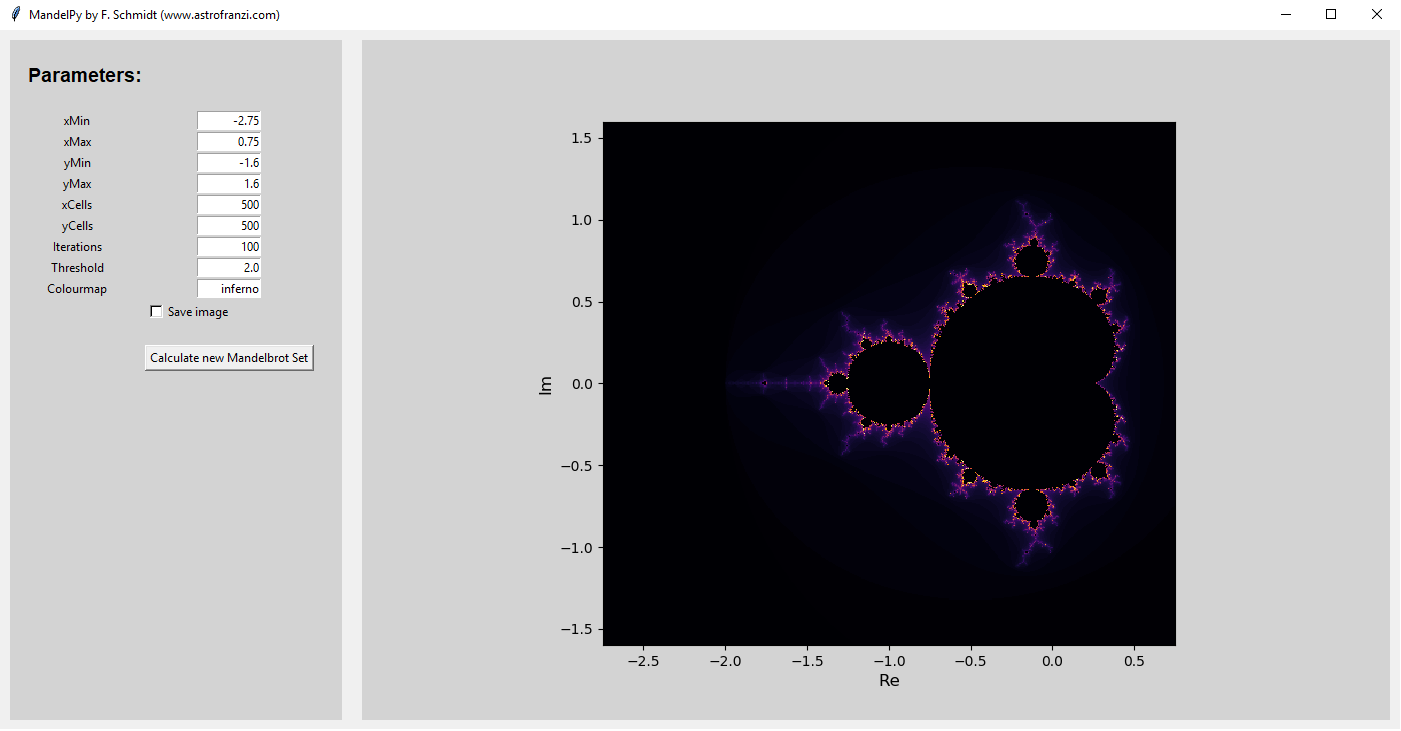
\includegraphics[width=\textwidth]{IMG/GUI.png}
		\caption{MandelPy GUI default view.}
\end{figure}\label{FIG_GUI}

Changing the {\code{Colourmap}} parameter but none of the others will only update the plot. Changing any of the other parameters will always lead to a recalculation of the Mandelbrot set.\\

Invalid input will lead to a message box popping up and pointing you to the source of the error. Close the message box, enter a correct value for the faulty parameter and click the "{\code{Calculate new Mandelbrot Set}}" button again.\\

Calculating a new Mandelbrot Set can take quite some time depending on your system specs, the resolution, and number of iterations set. Once the Mandelbrot Set has been calculated a message box will pop up. Close the box and the plot will be updated and (if enabled) the image will be exported (this might also take a couple of seconds if the dataset is very large).




\section{Code Structure}

The {\code{MandelPy}} source code is open source and split into the following python files:

\subsection{Jupyter Notebook}

\subsubsection{{\code{MandelPy.ipynb}}}
The Jupyter Notebook is probably the easiest to understand as the entire code is contained within one Notebook and flows rather linearly.\\
The first block imports all necessary libraries, followed by a block setting the initial parameters and another block containing two functions necessary to calculate the Mandelbrot Set.\\
The main code sets up the computational domain based on the input parameters, calculates the Mandelbrot Set and then visualizes it.\\
To update the plot, change the variables in the {\code{Input Parameters}} block and run all cells below it.

\subsection{Widget}

The source code for the widget is split into several source files to render the code less convoluted.

\subsubsection{{\code{varGlobal.py}}}
This script contains global variables for the entire code. They are equivalent to the input parameters of the Jupyter Notebook. Most of them are only used for the very first plot. You can change them directly inside the script or use the widget to update the plot.

\subsubsection{{\code{MandelPy.py}}}
This script contains the main driver of the code. It initializes the widget and starts the GUI.

\subsubsection{{\code{fctMandelbrotSet.py}}}
This script contains the same two functions used in the Jupyter Notebook to calculate the Mandelbrot Set.

\subsubsection{{\code{classWidget.py}}}
This script is probably the messiest one (and the unfortunate result of trying to learn {\code{tkinter}} in a day) and handles the GUI. It contains the class {\code{Widget}} which generates the parameter frame and the plot frame in the GUI, calculates the first Mandelbrot Set and displays the plot. The input boxes, the tick box, and the button are also controlled from within {\code{Widget}}. Once the button is clicked, {\code{ButtonClicked}} is called which will first make sure all entries are valid (and throw exceptions if that is not the case) and then test whether the plot can simply be updated or if a new Mandelbrot Set needs to be calculated. At the end of the member function, the {\code{Python}} calls the function {\code{RefreshFigure}} which will update the plot using either the old Mandelbrot Set with a new colour scheme or the newly calculated Mandelbrot Set. Finally, the plot is saved as a png file with the same naming convention as the Jupyter Notebook. Images exported via the GUI will be of higher quality as those obtained through the Jupyter Notebook or screenshots of the widget.



\section{Examples}

\subsubsection{Variation of the Grid Size}

\begin{figure}[H]
\centering
\begin{subfigure}{.45\textwidth}
  \centering
  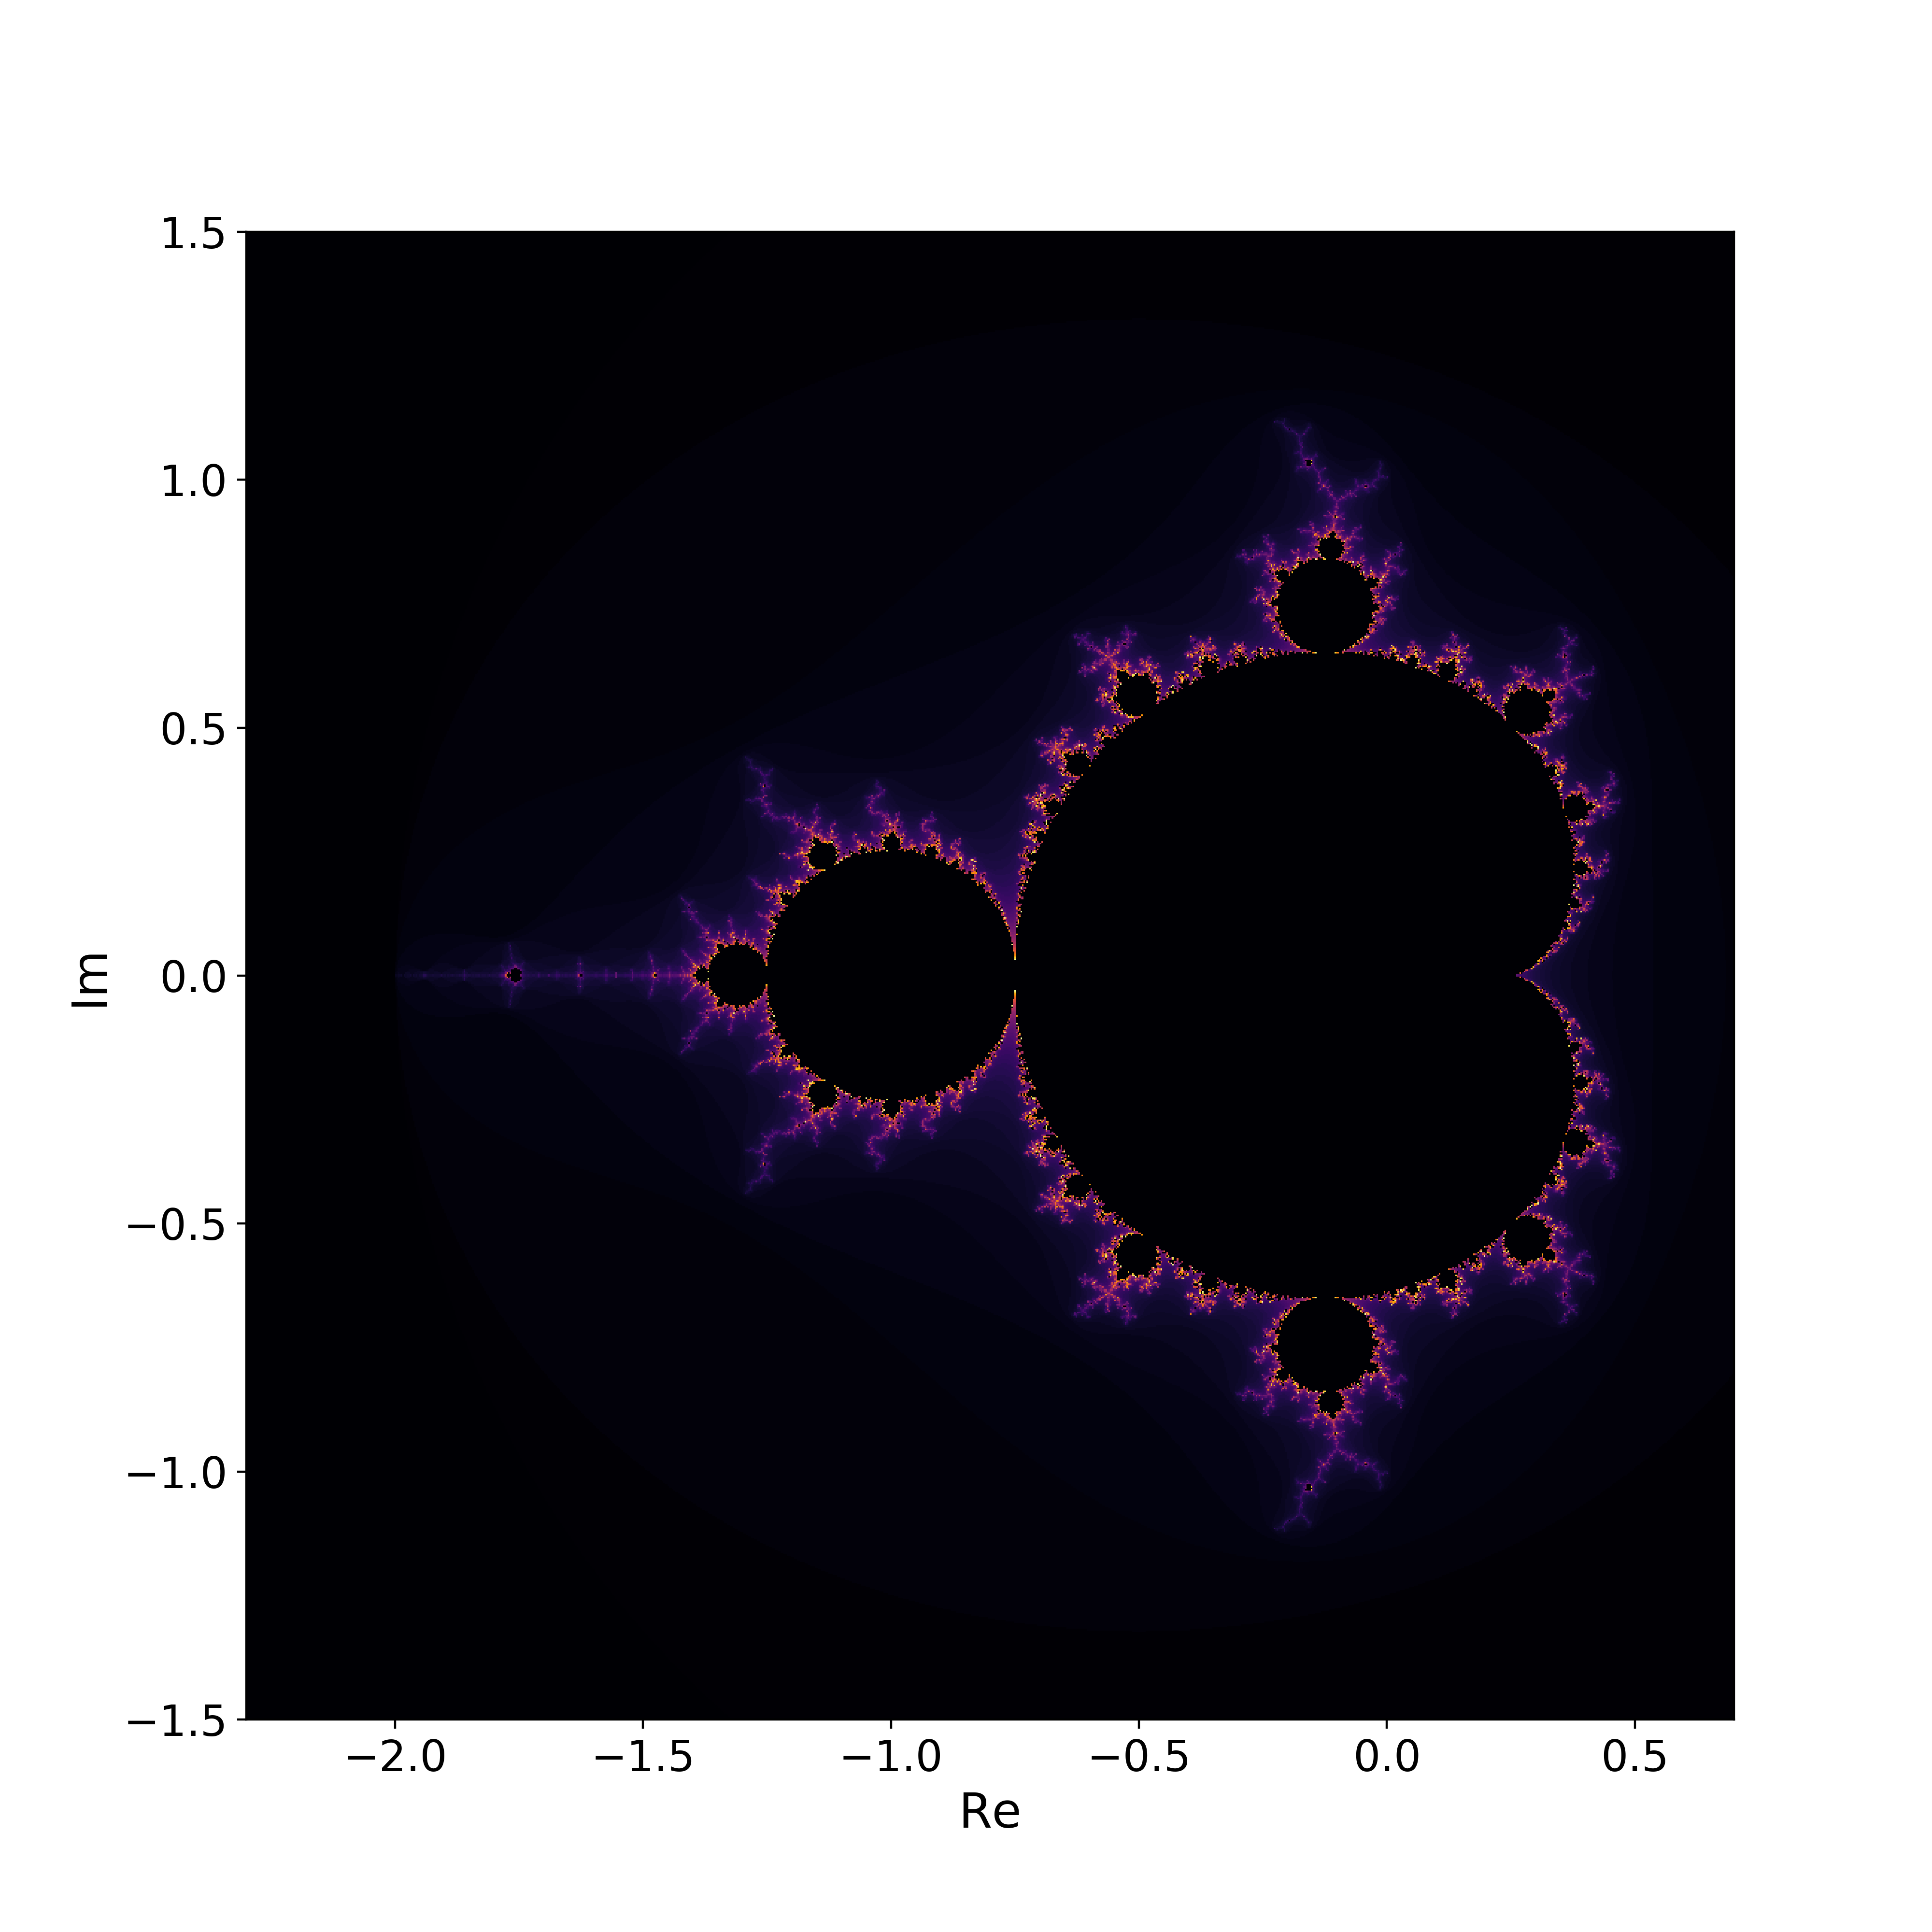
\includegraphics[width=\linewidth]{IMG/GridSize1.png}
  \caption{Original Mandelbrot Set.}
\end{subfigure}%
\begin{subfigure}{.45\textwidth}
  \centering
  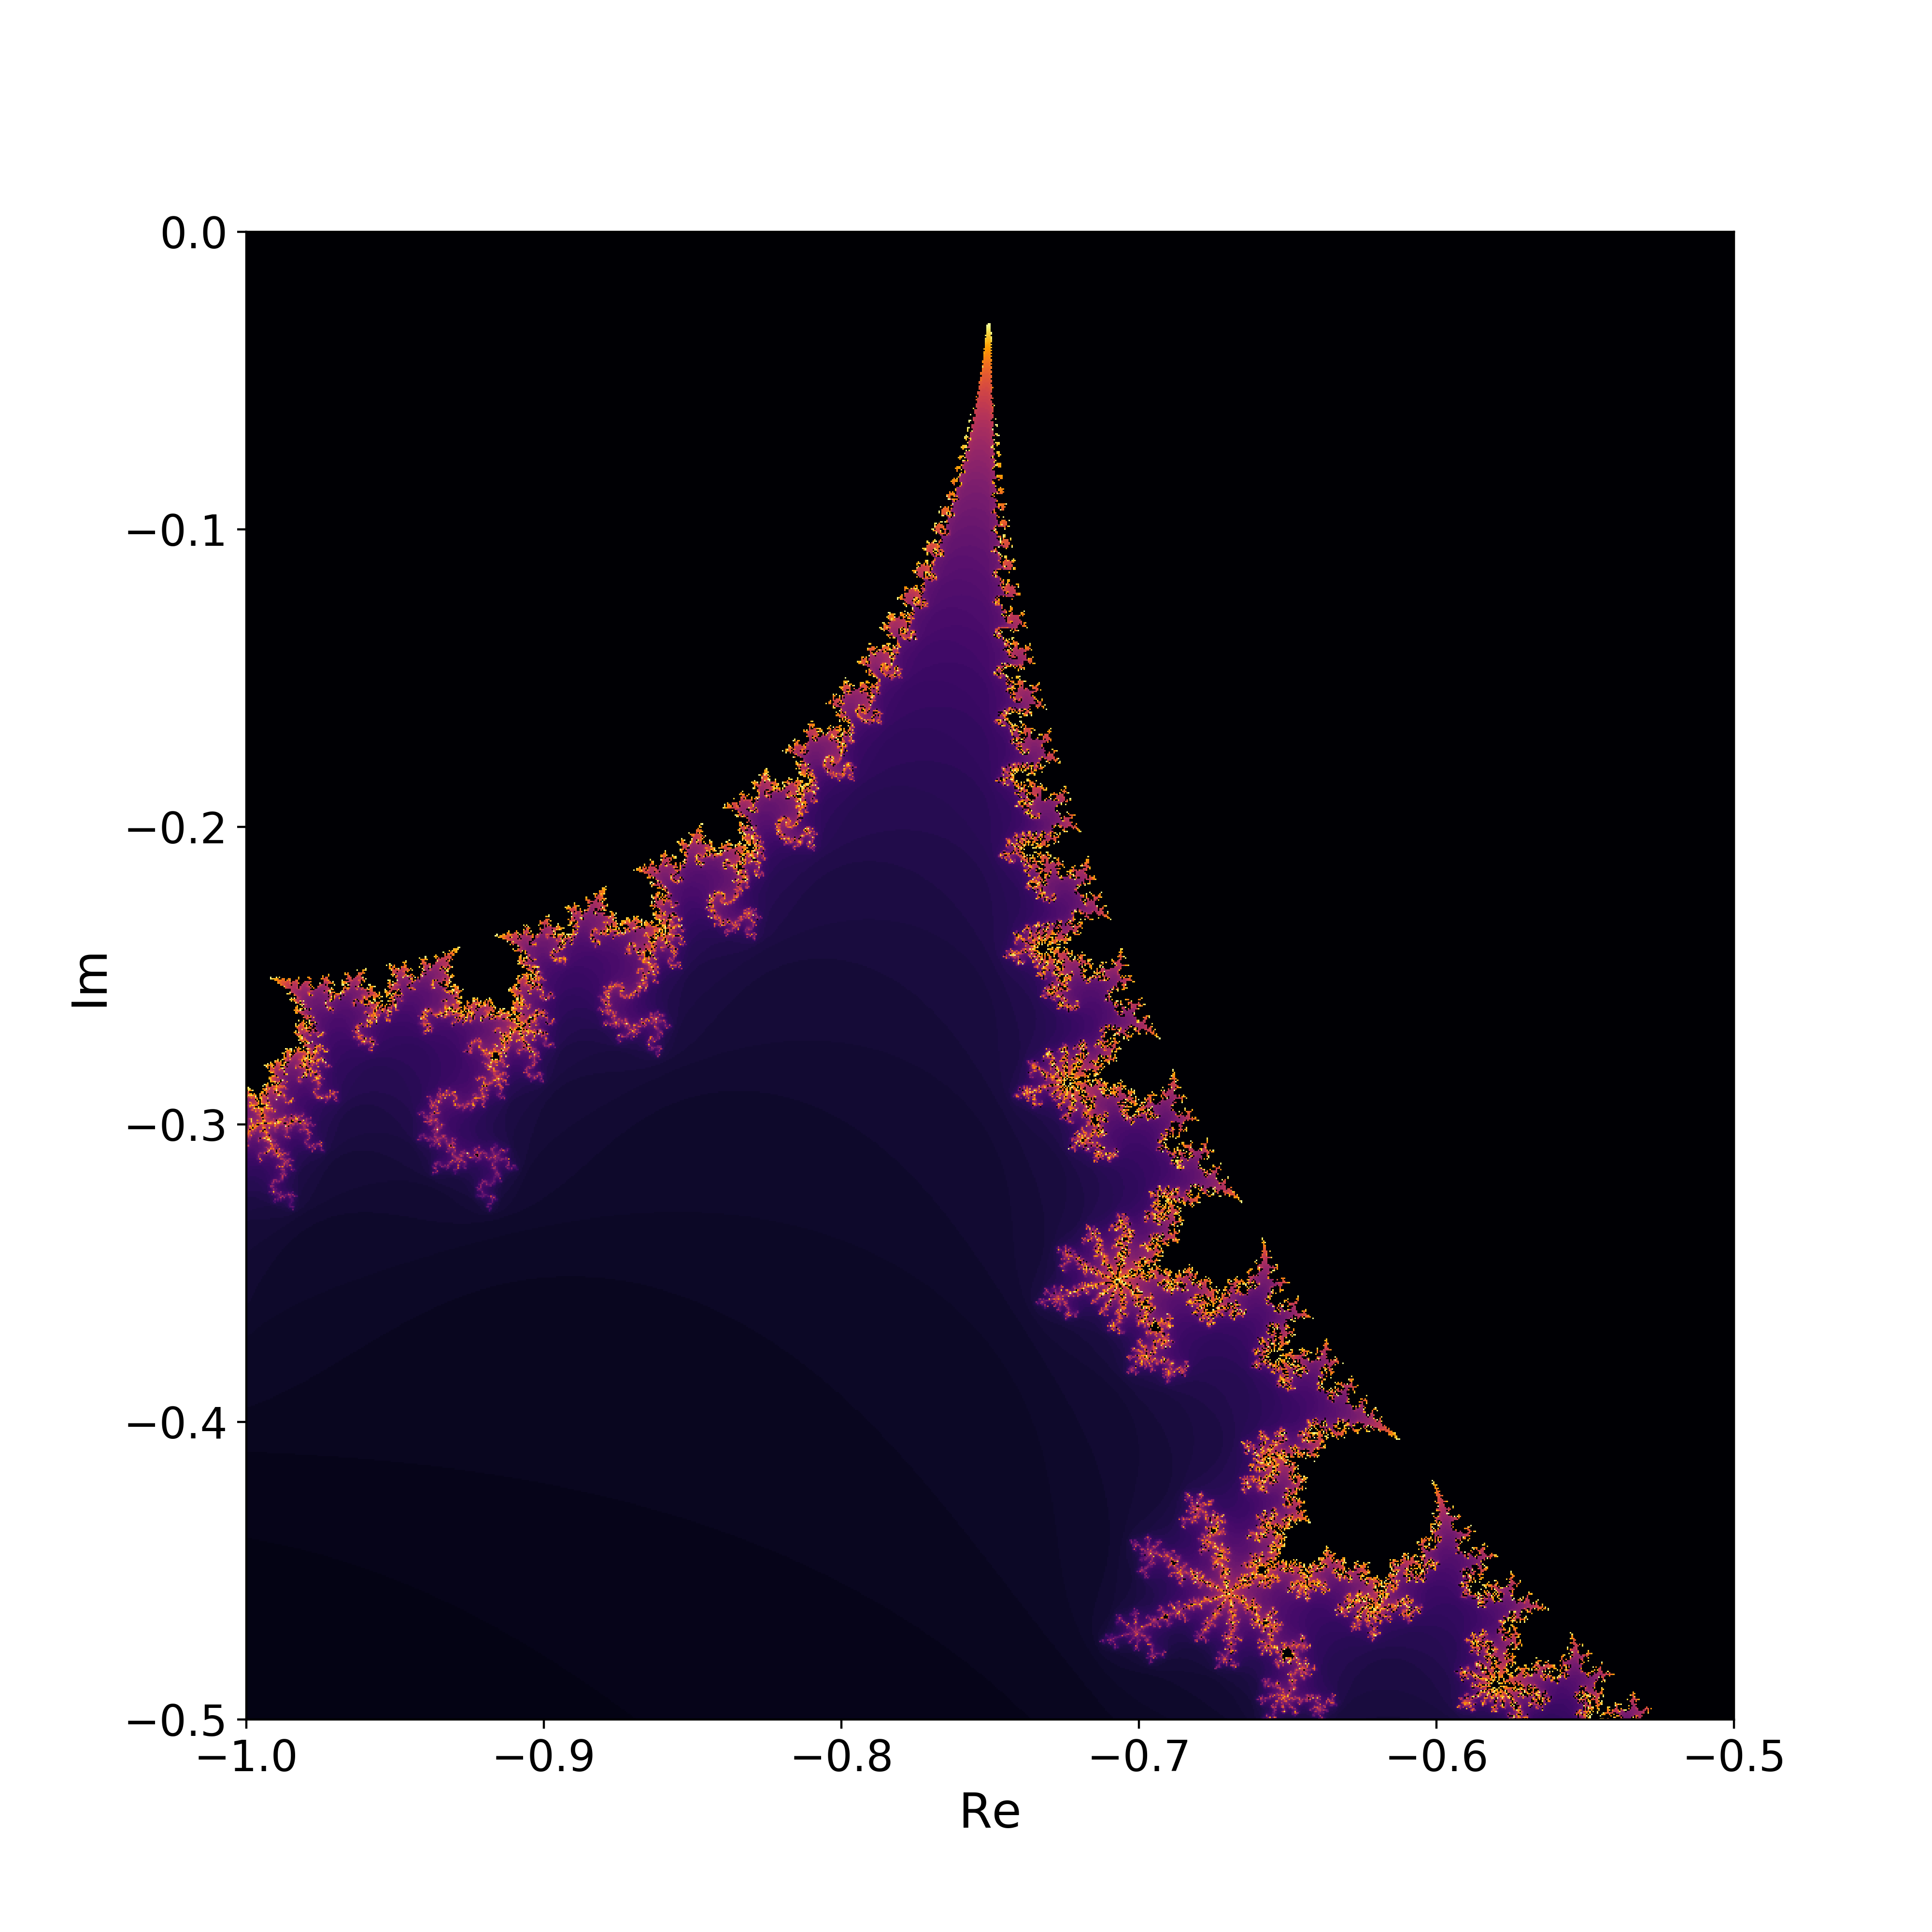
\includegraphics[width=\linewidth]{IMG/GridSize2.png}
  \caption{First zoom.}
\end{subfigure}
\begin{subfigure}{.45\textwidth}
  \centering
  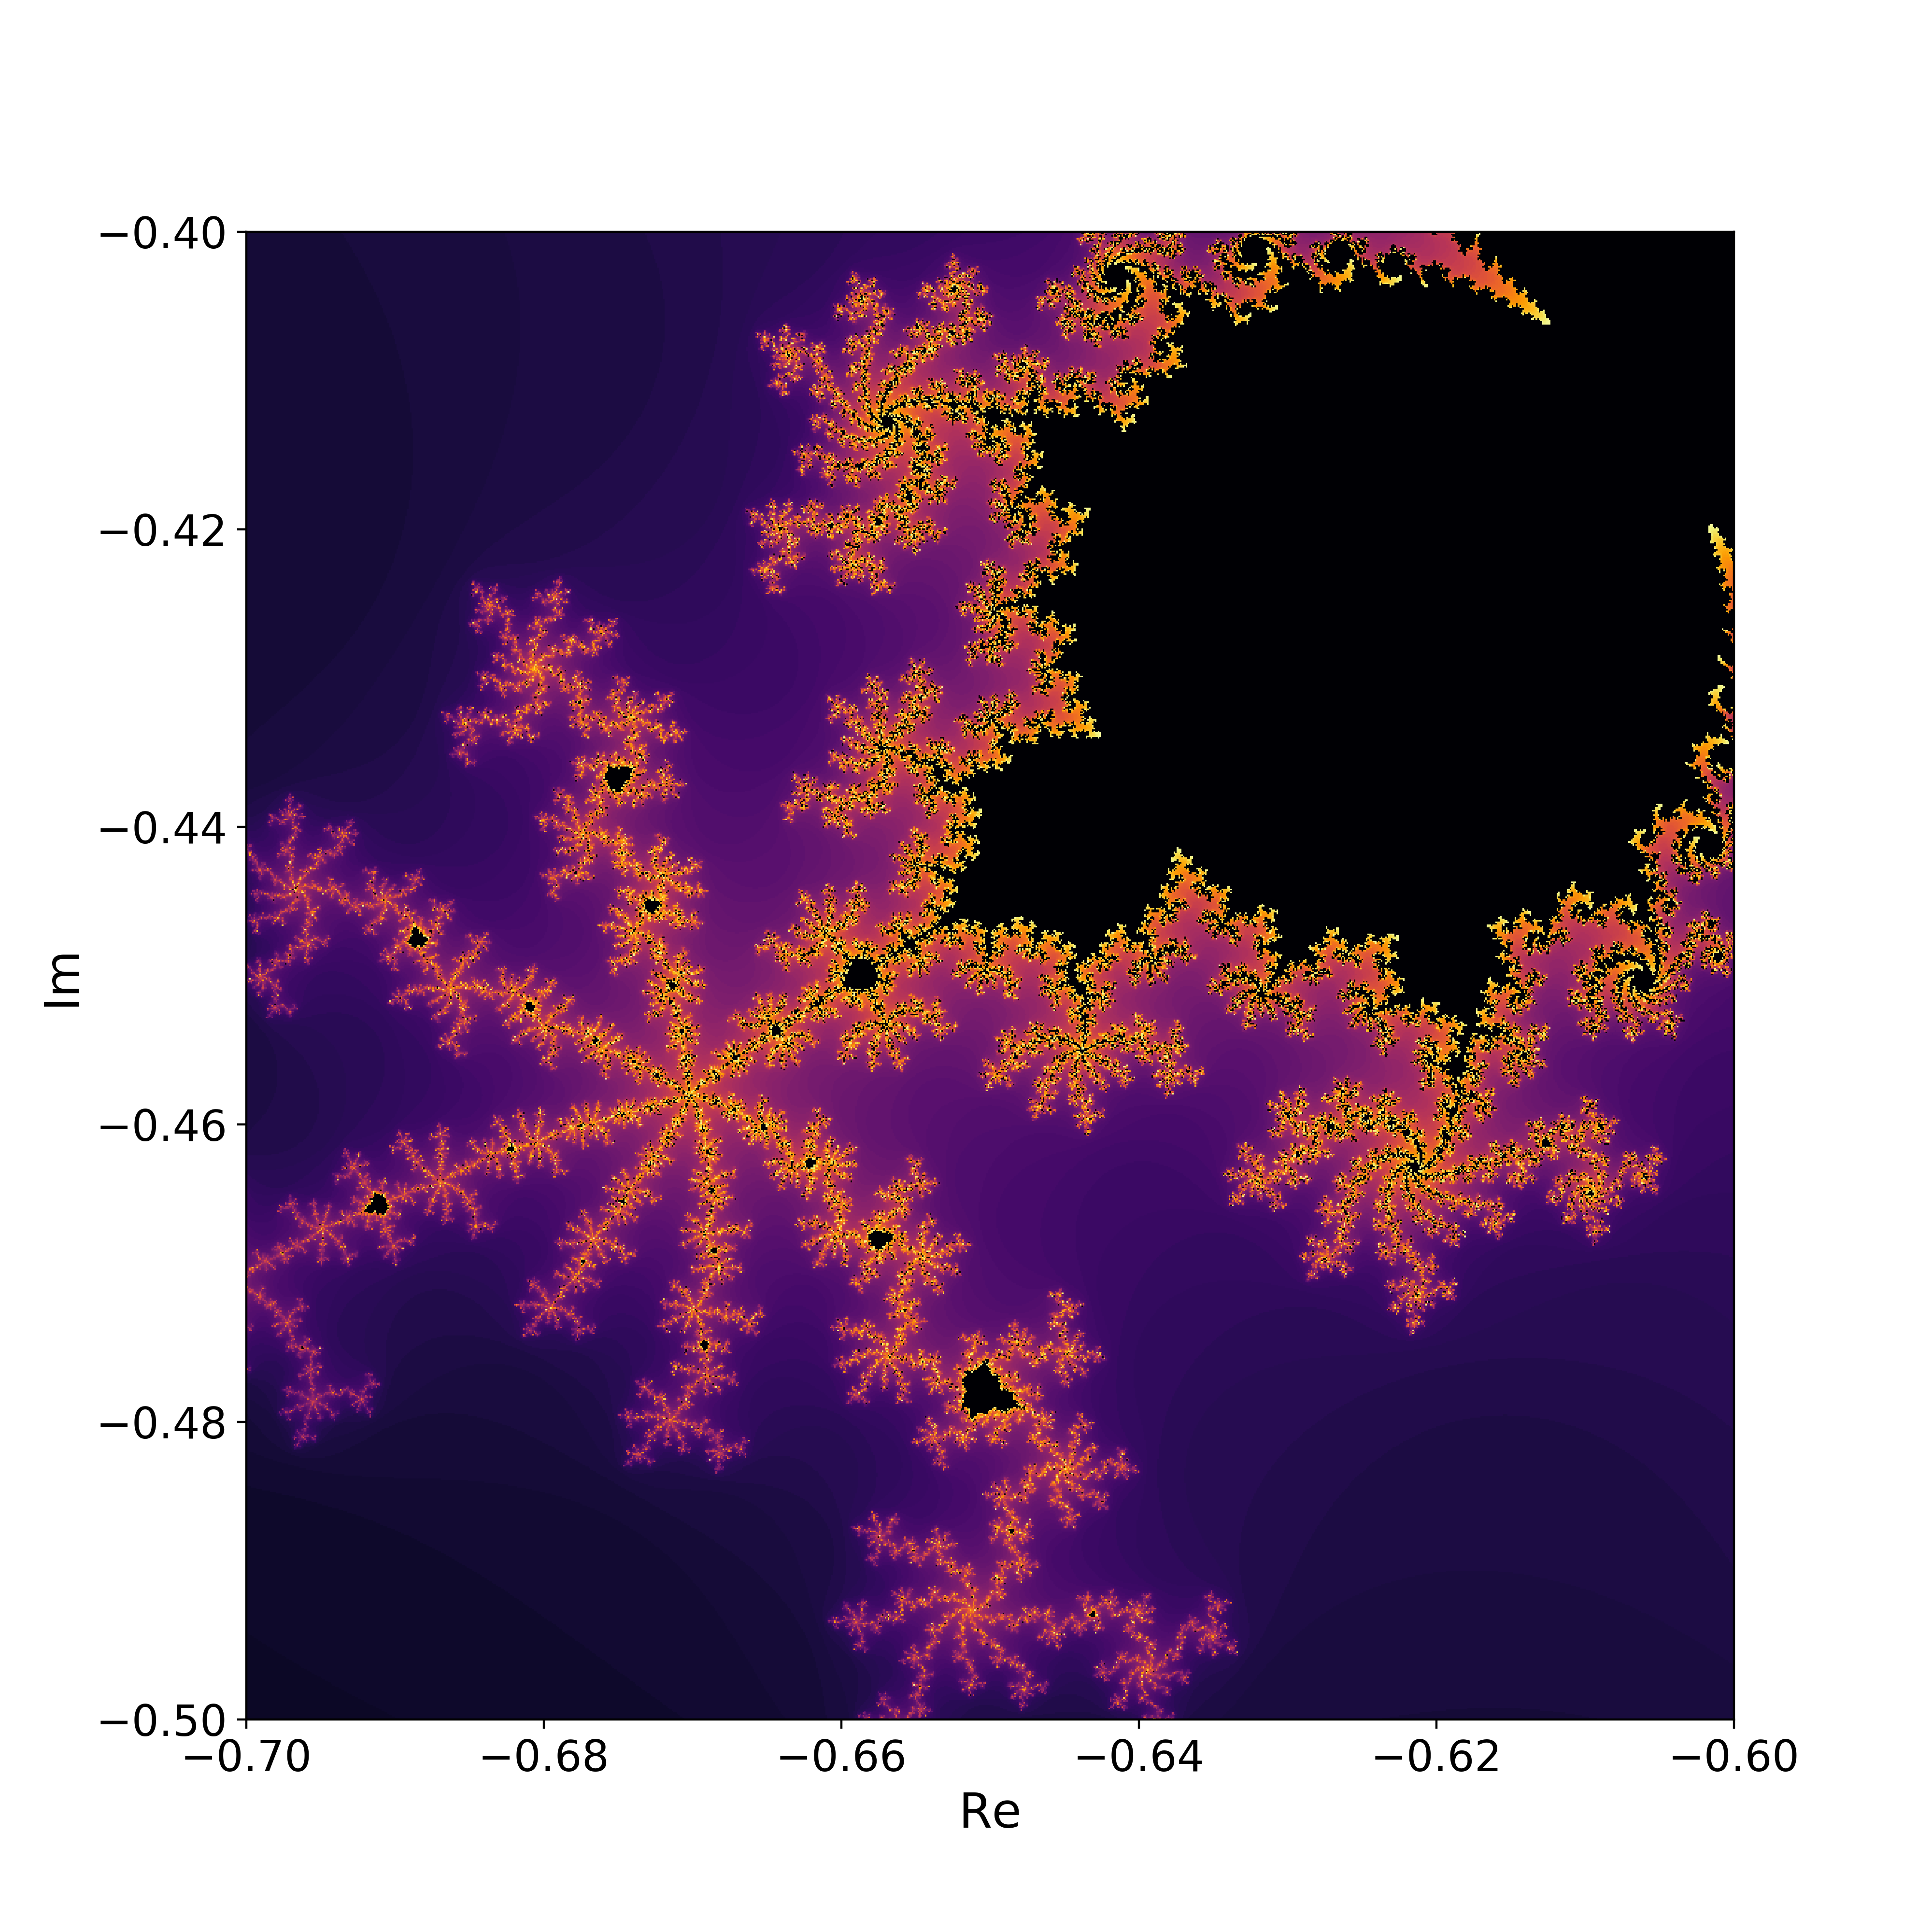
\includegraphics[width=\linewidth]{IMG/GridSize3.png}
  \caption{Second zoom.}
\end{subfigure}
\begin{subfigure}{.45\textwidth}
  \centering
  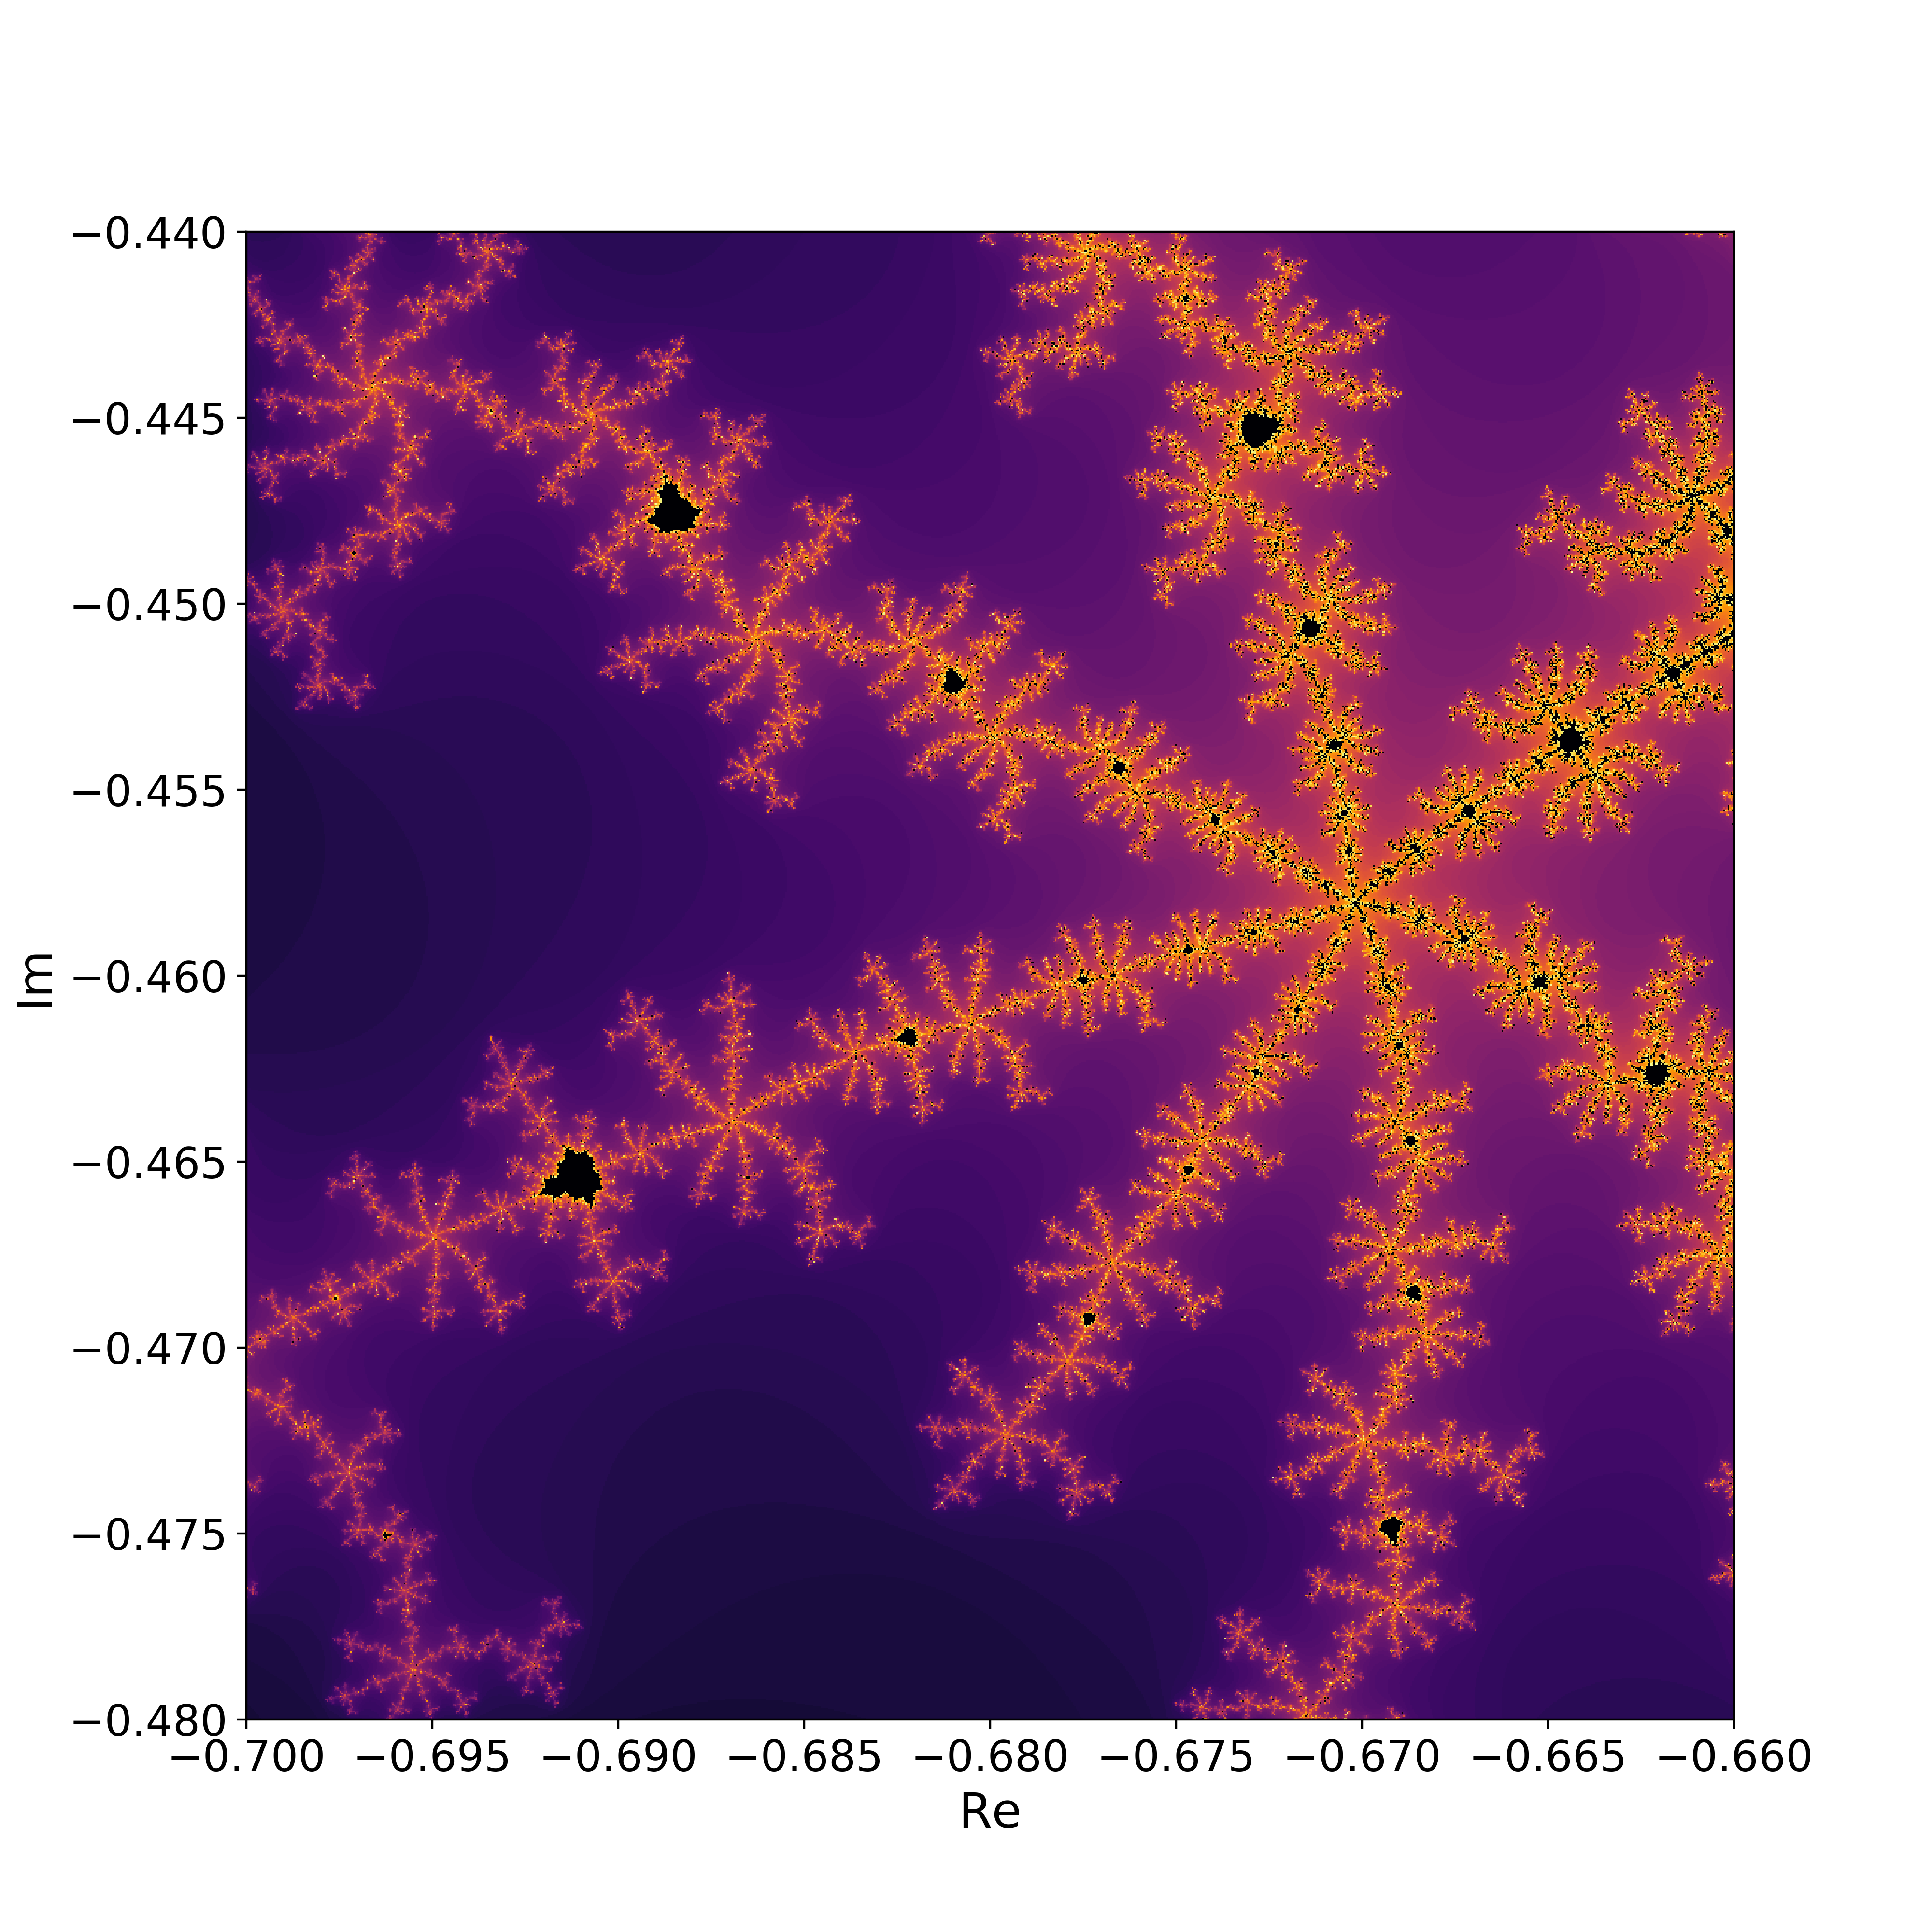
\includegraphics[width=\linewidth]{IMG/GridSize4.png}
  \caption{Third zoom.}
\end{subfigure}
\caption{Variation of the grid size.}
\label{FIG_GridSize}
\end{figure}


\newpage
\subsubsection{Variation of the Resolution}

\begin{figure}[H]
\centering
\begin{subfigure}{.45\textwidth}
  \centering
  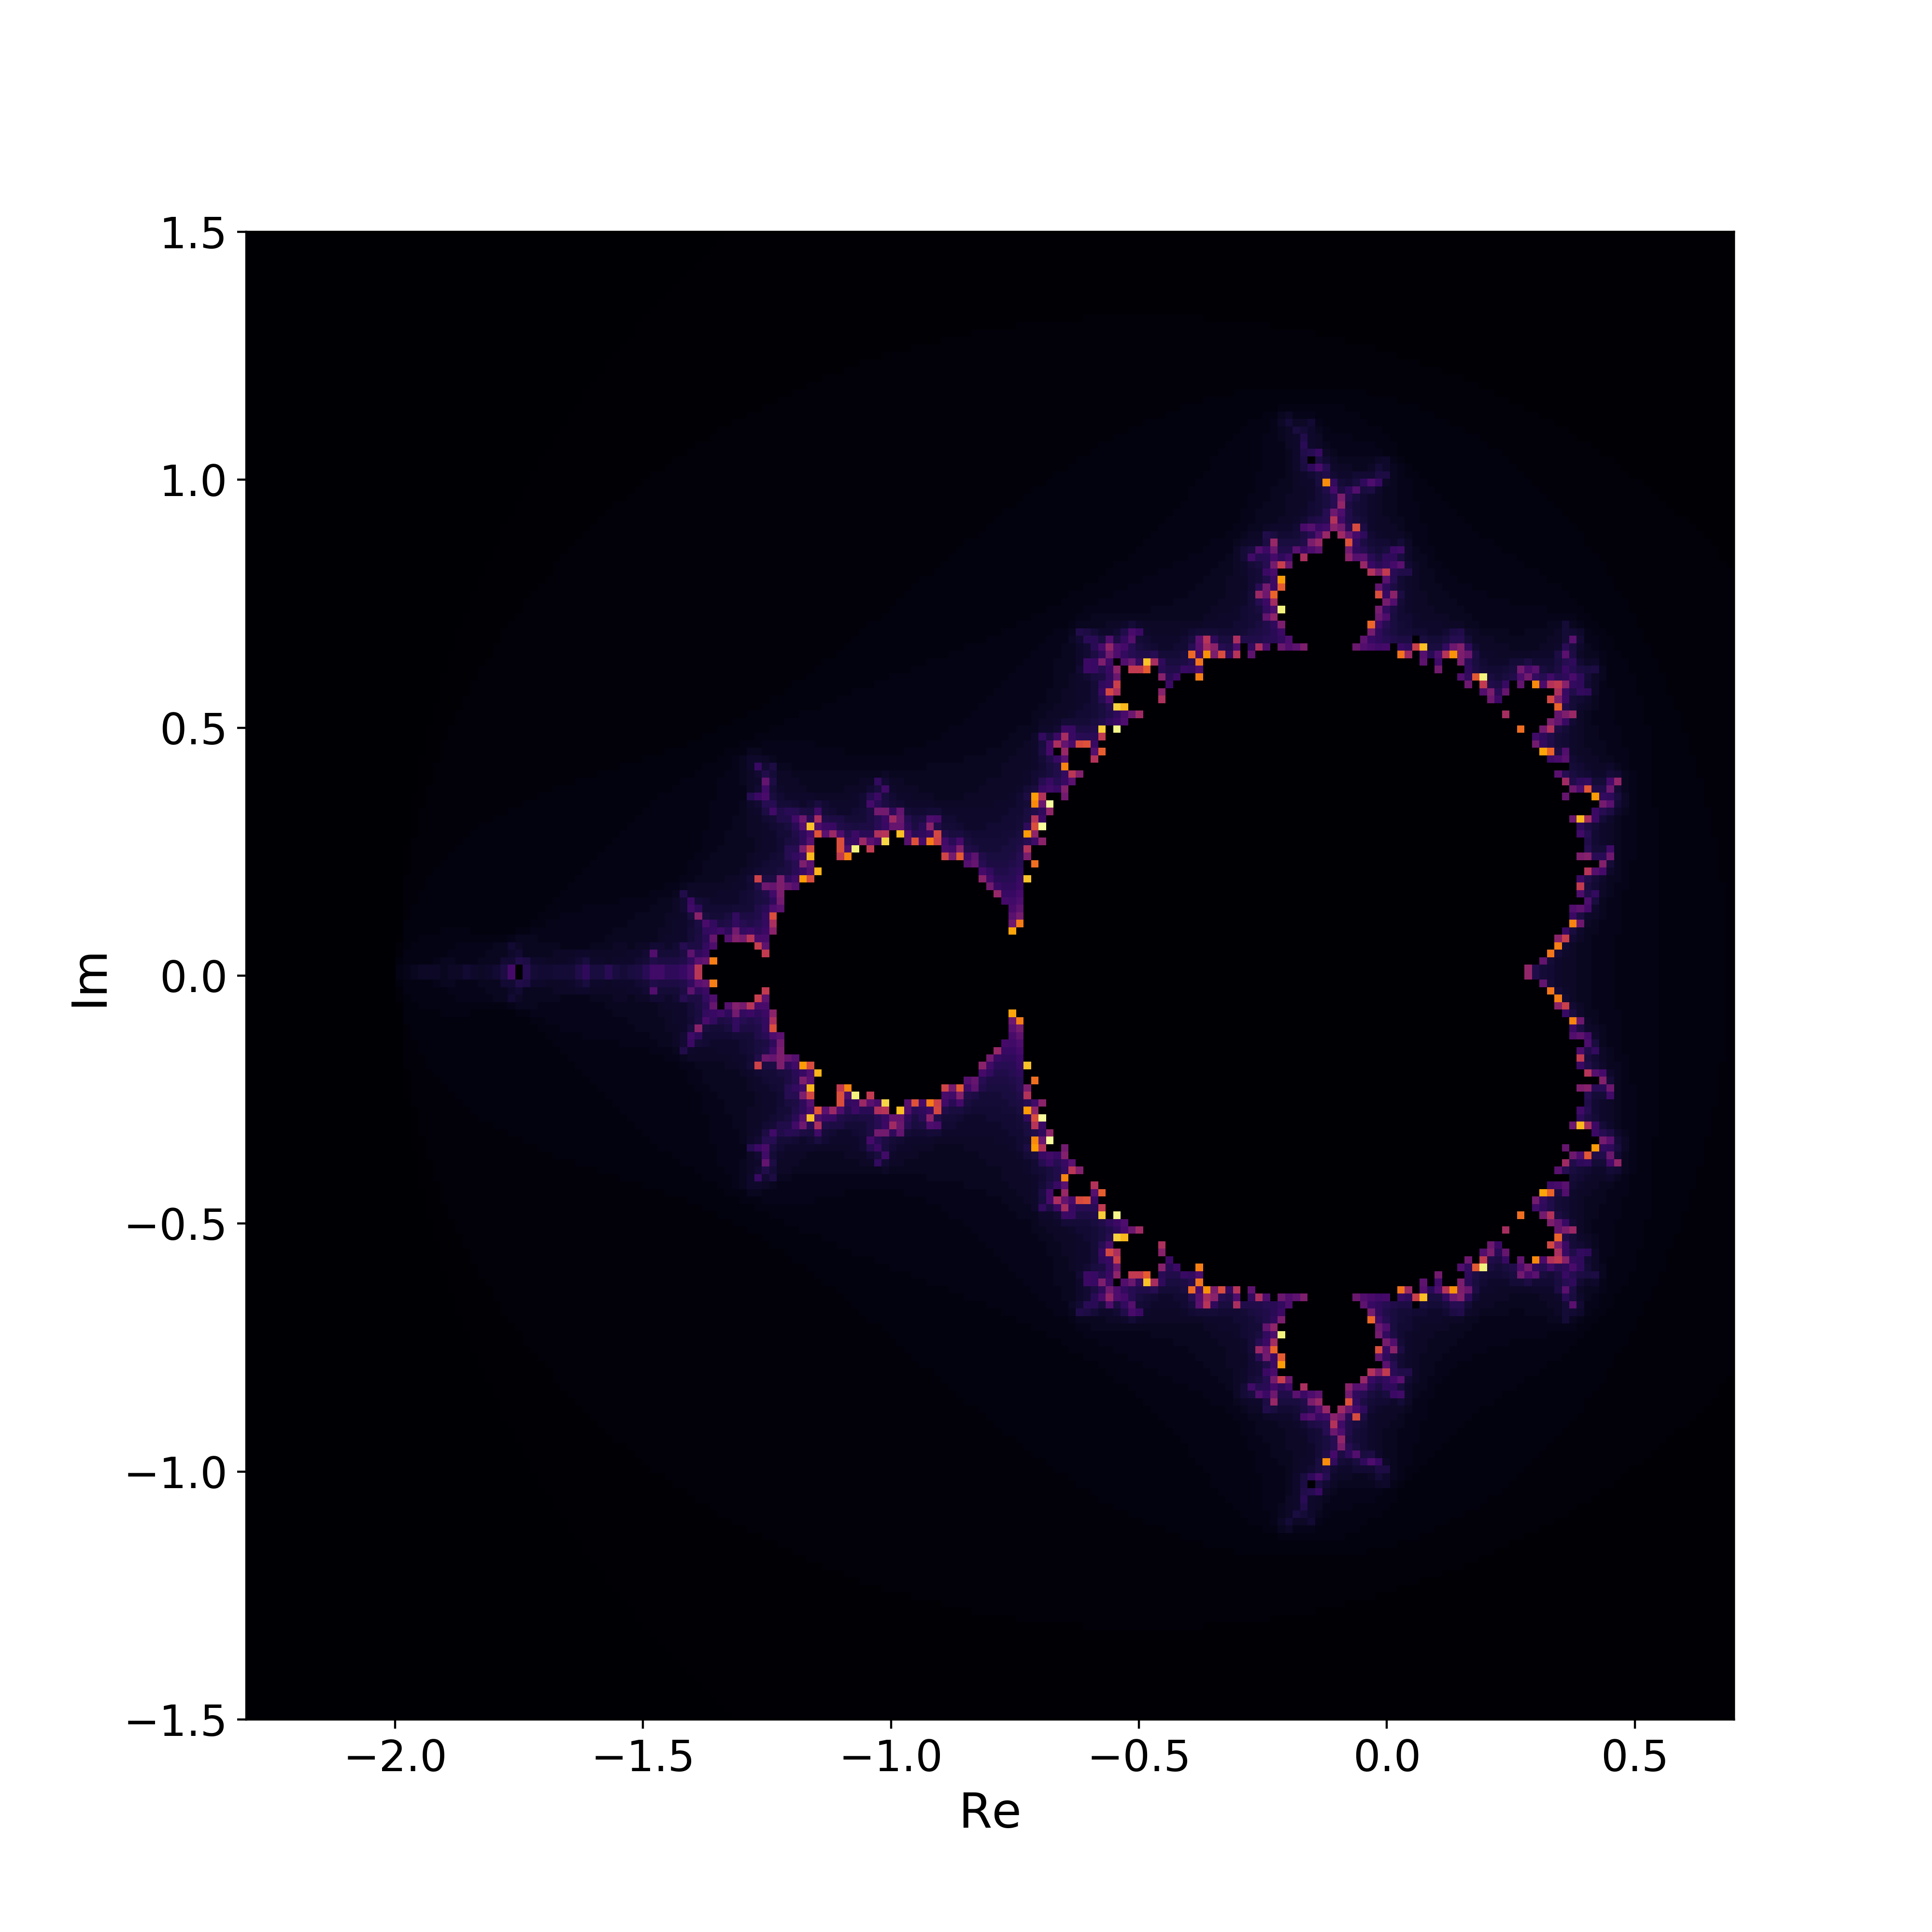
\includegraphics[width=\linewidth]{IMG/Res1.png}
  \caption{Grid Size $200 \, \times \, 200$.}
\end{subfigure}%
\begin{subfigure}{.45\textwidth}
  \centering
  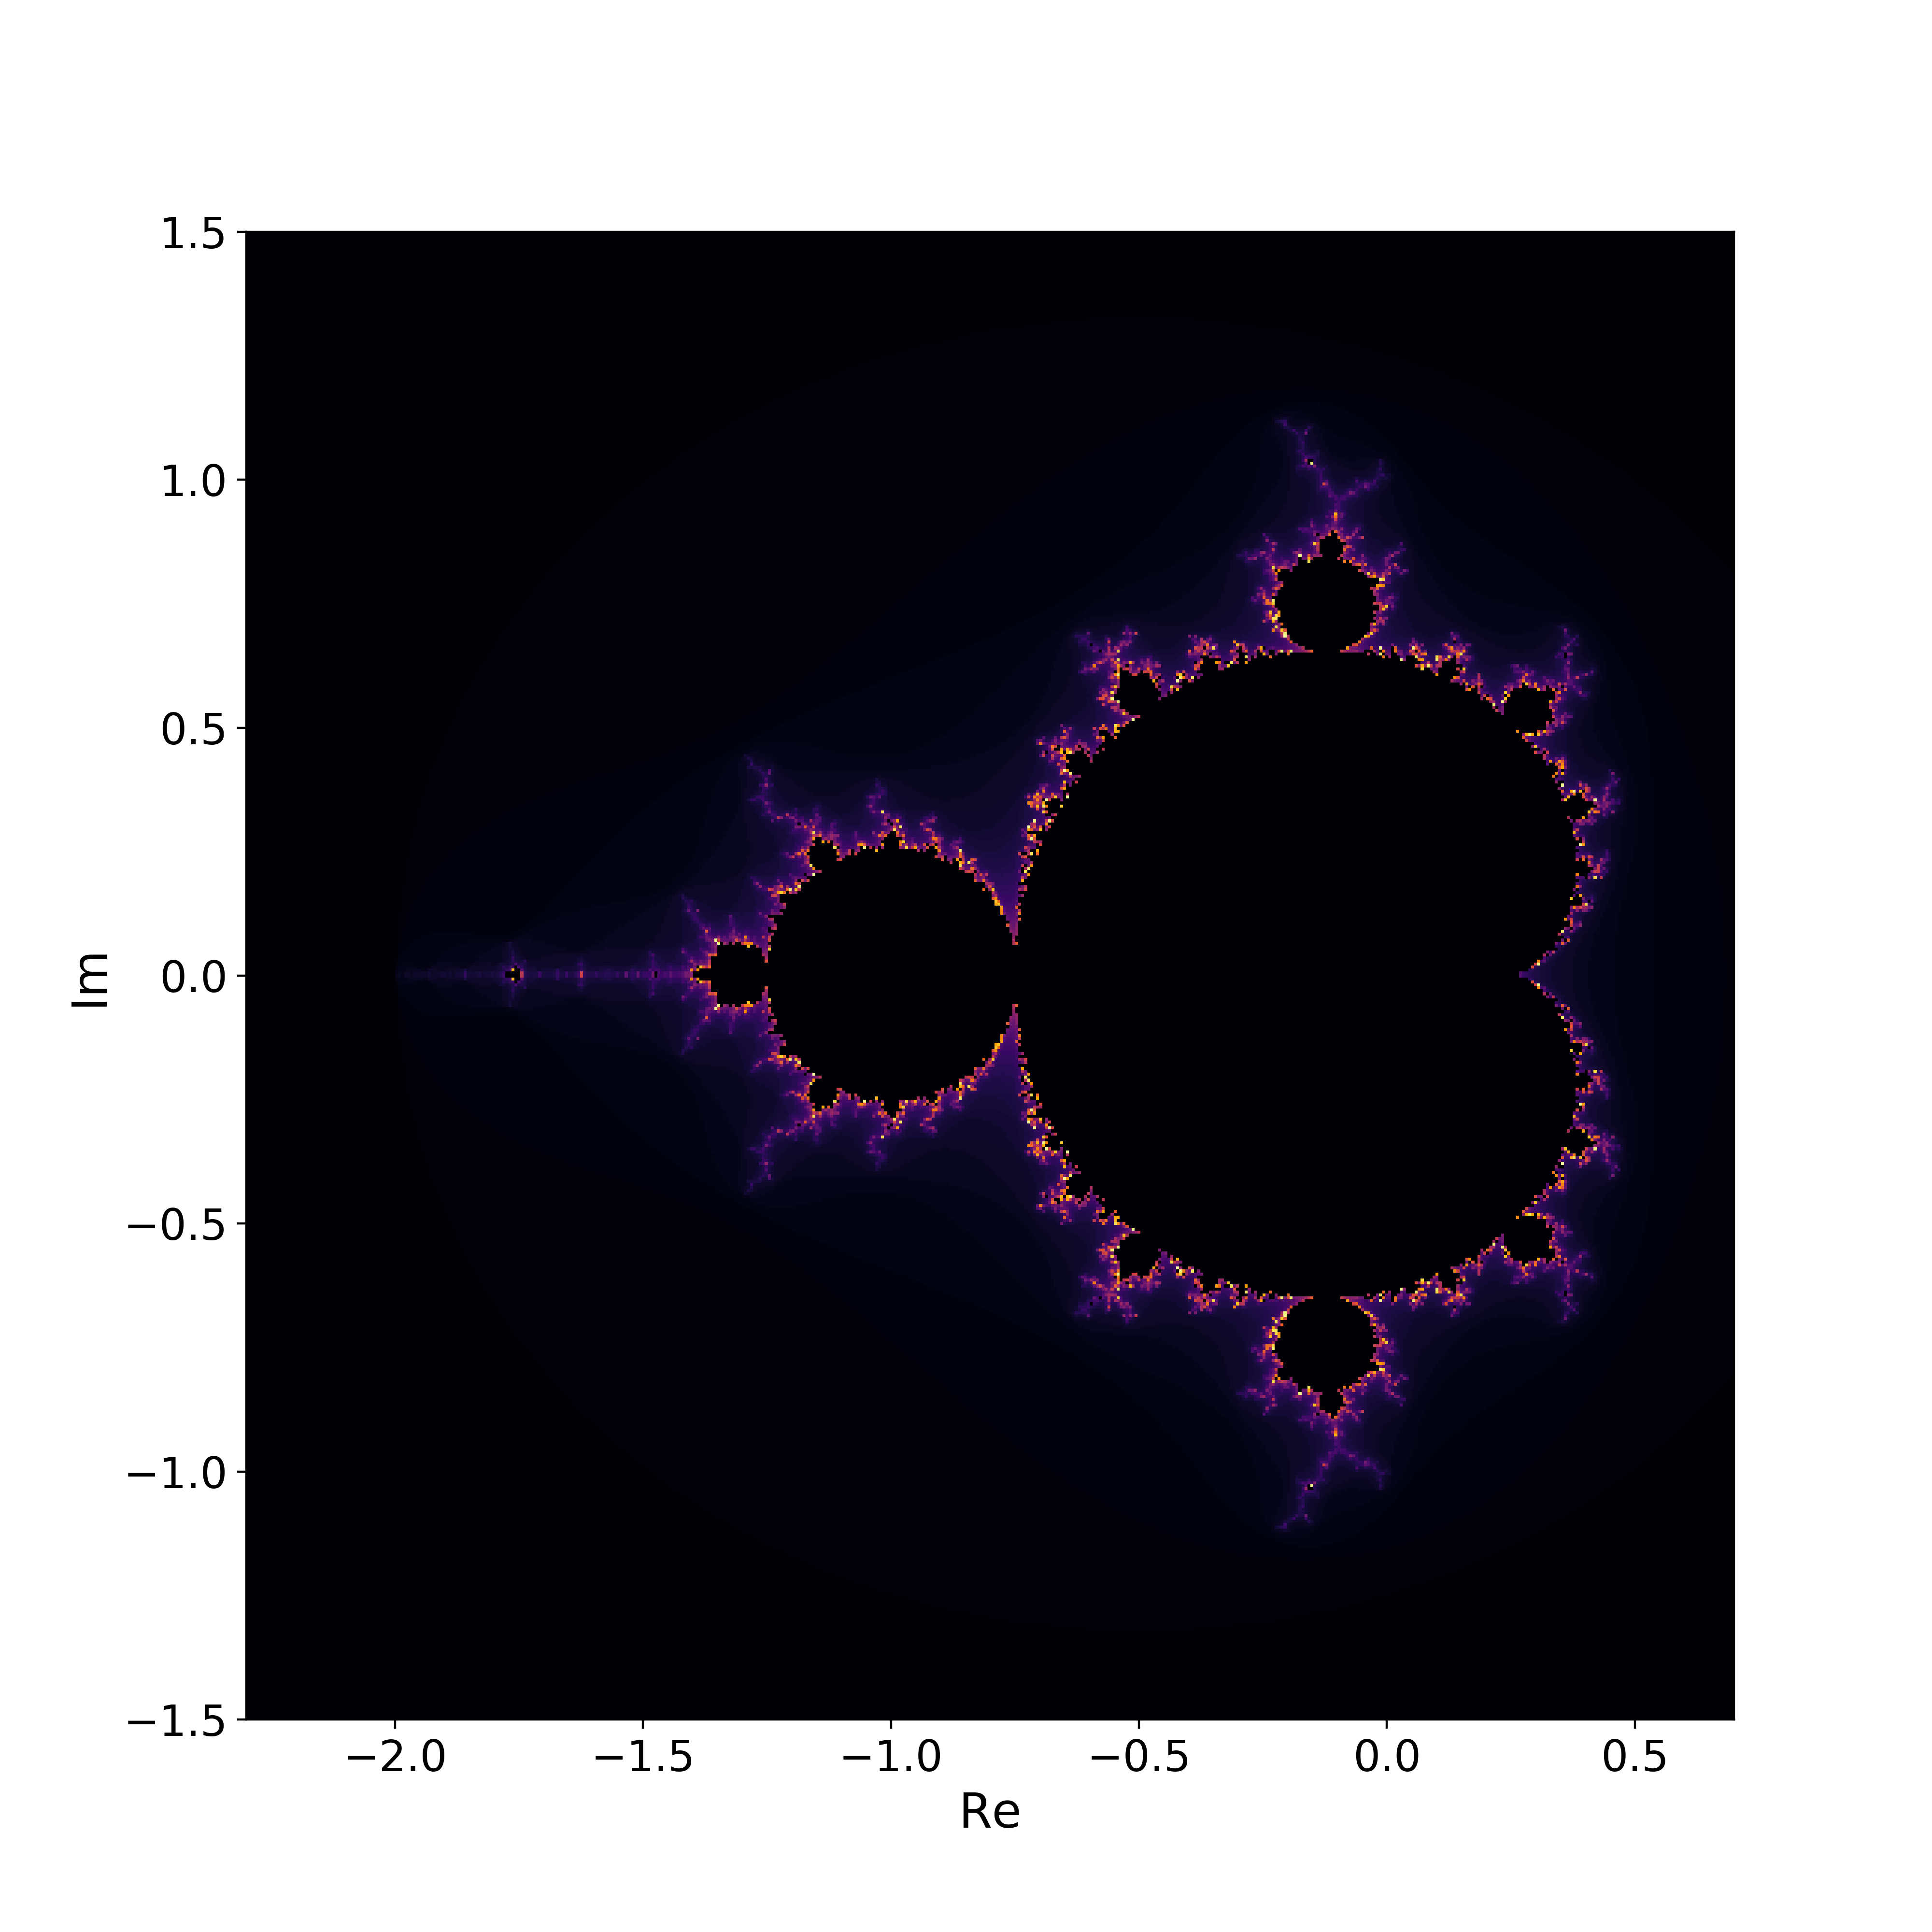
\includegraphics[width=\linewidth]{IMG/Res2.png}
  \caption{Grid Size $500 \, \times \, 500$.}
\end{subfigure}
\begin{subfigure}{.45\textwidth}
  \centering
  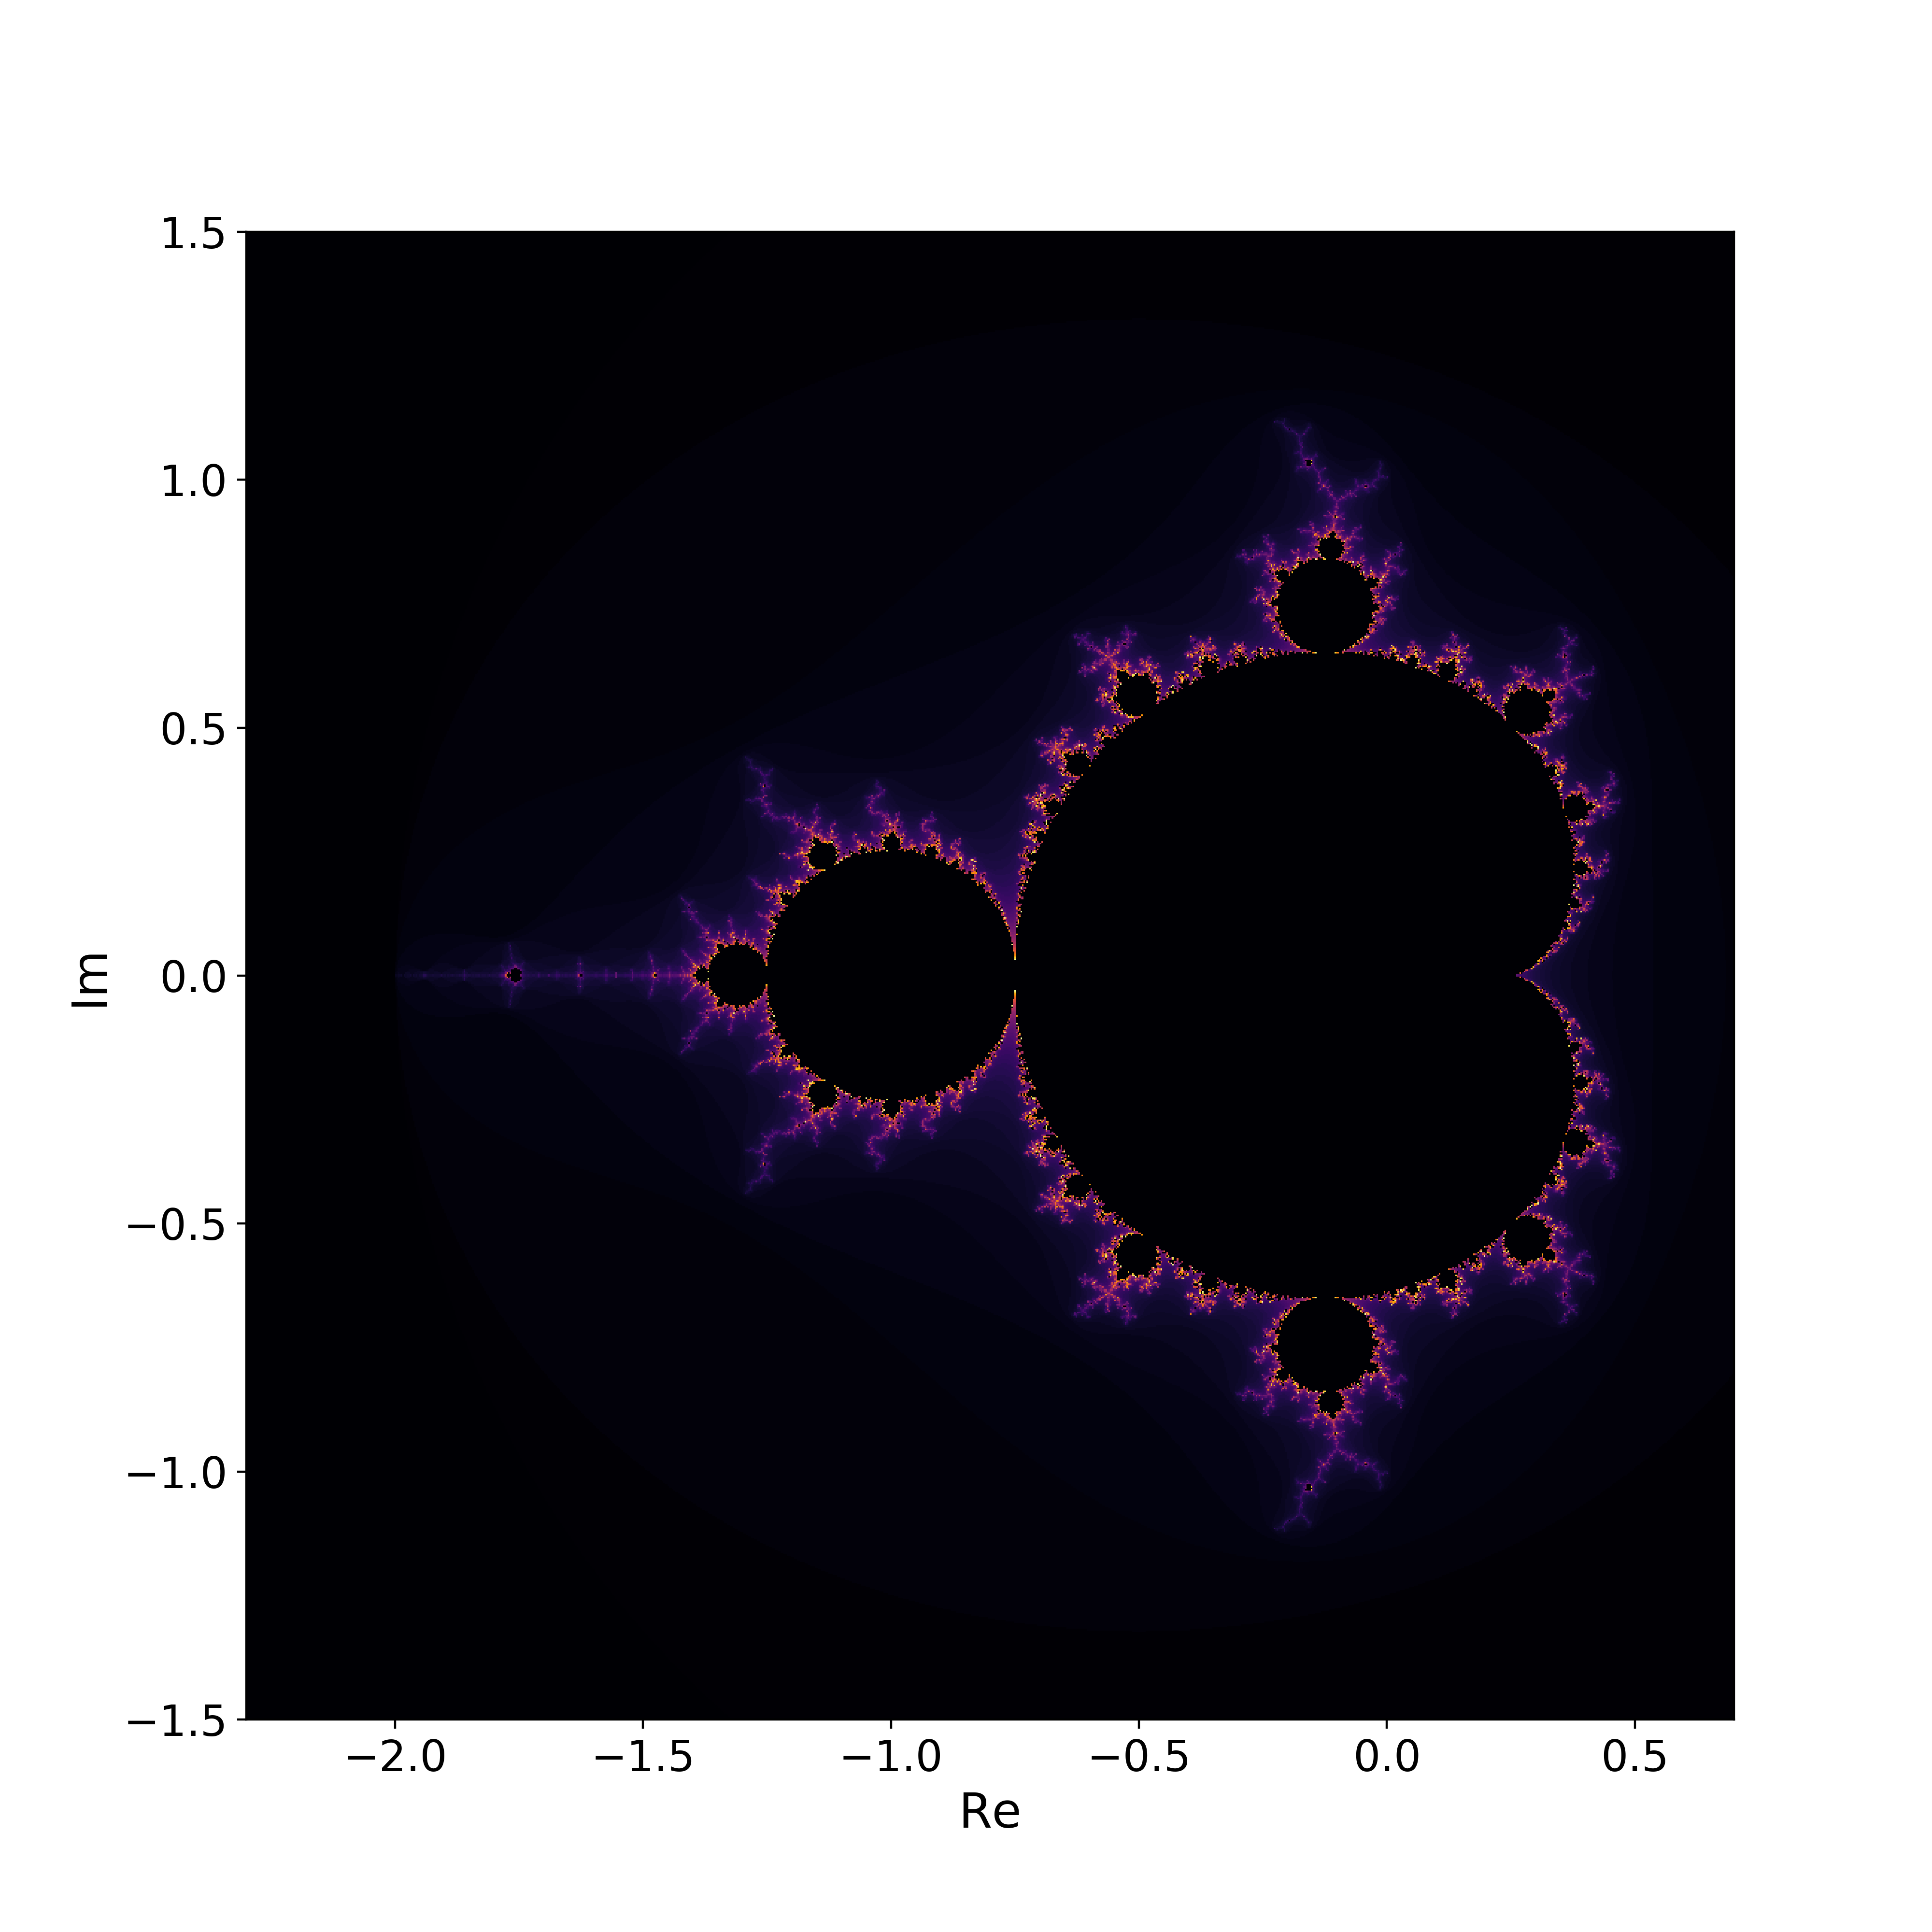
\includegraphics[width=\linewidth]{IMG/Res3.png}
  \caption{Grid Size $1000 \, \times \, 1000$.}
\end{subfigure}
\begin{subfigure}{.45\textwidth}
  \centering
  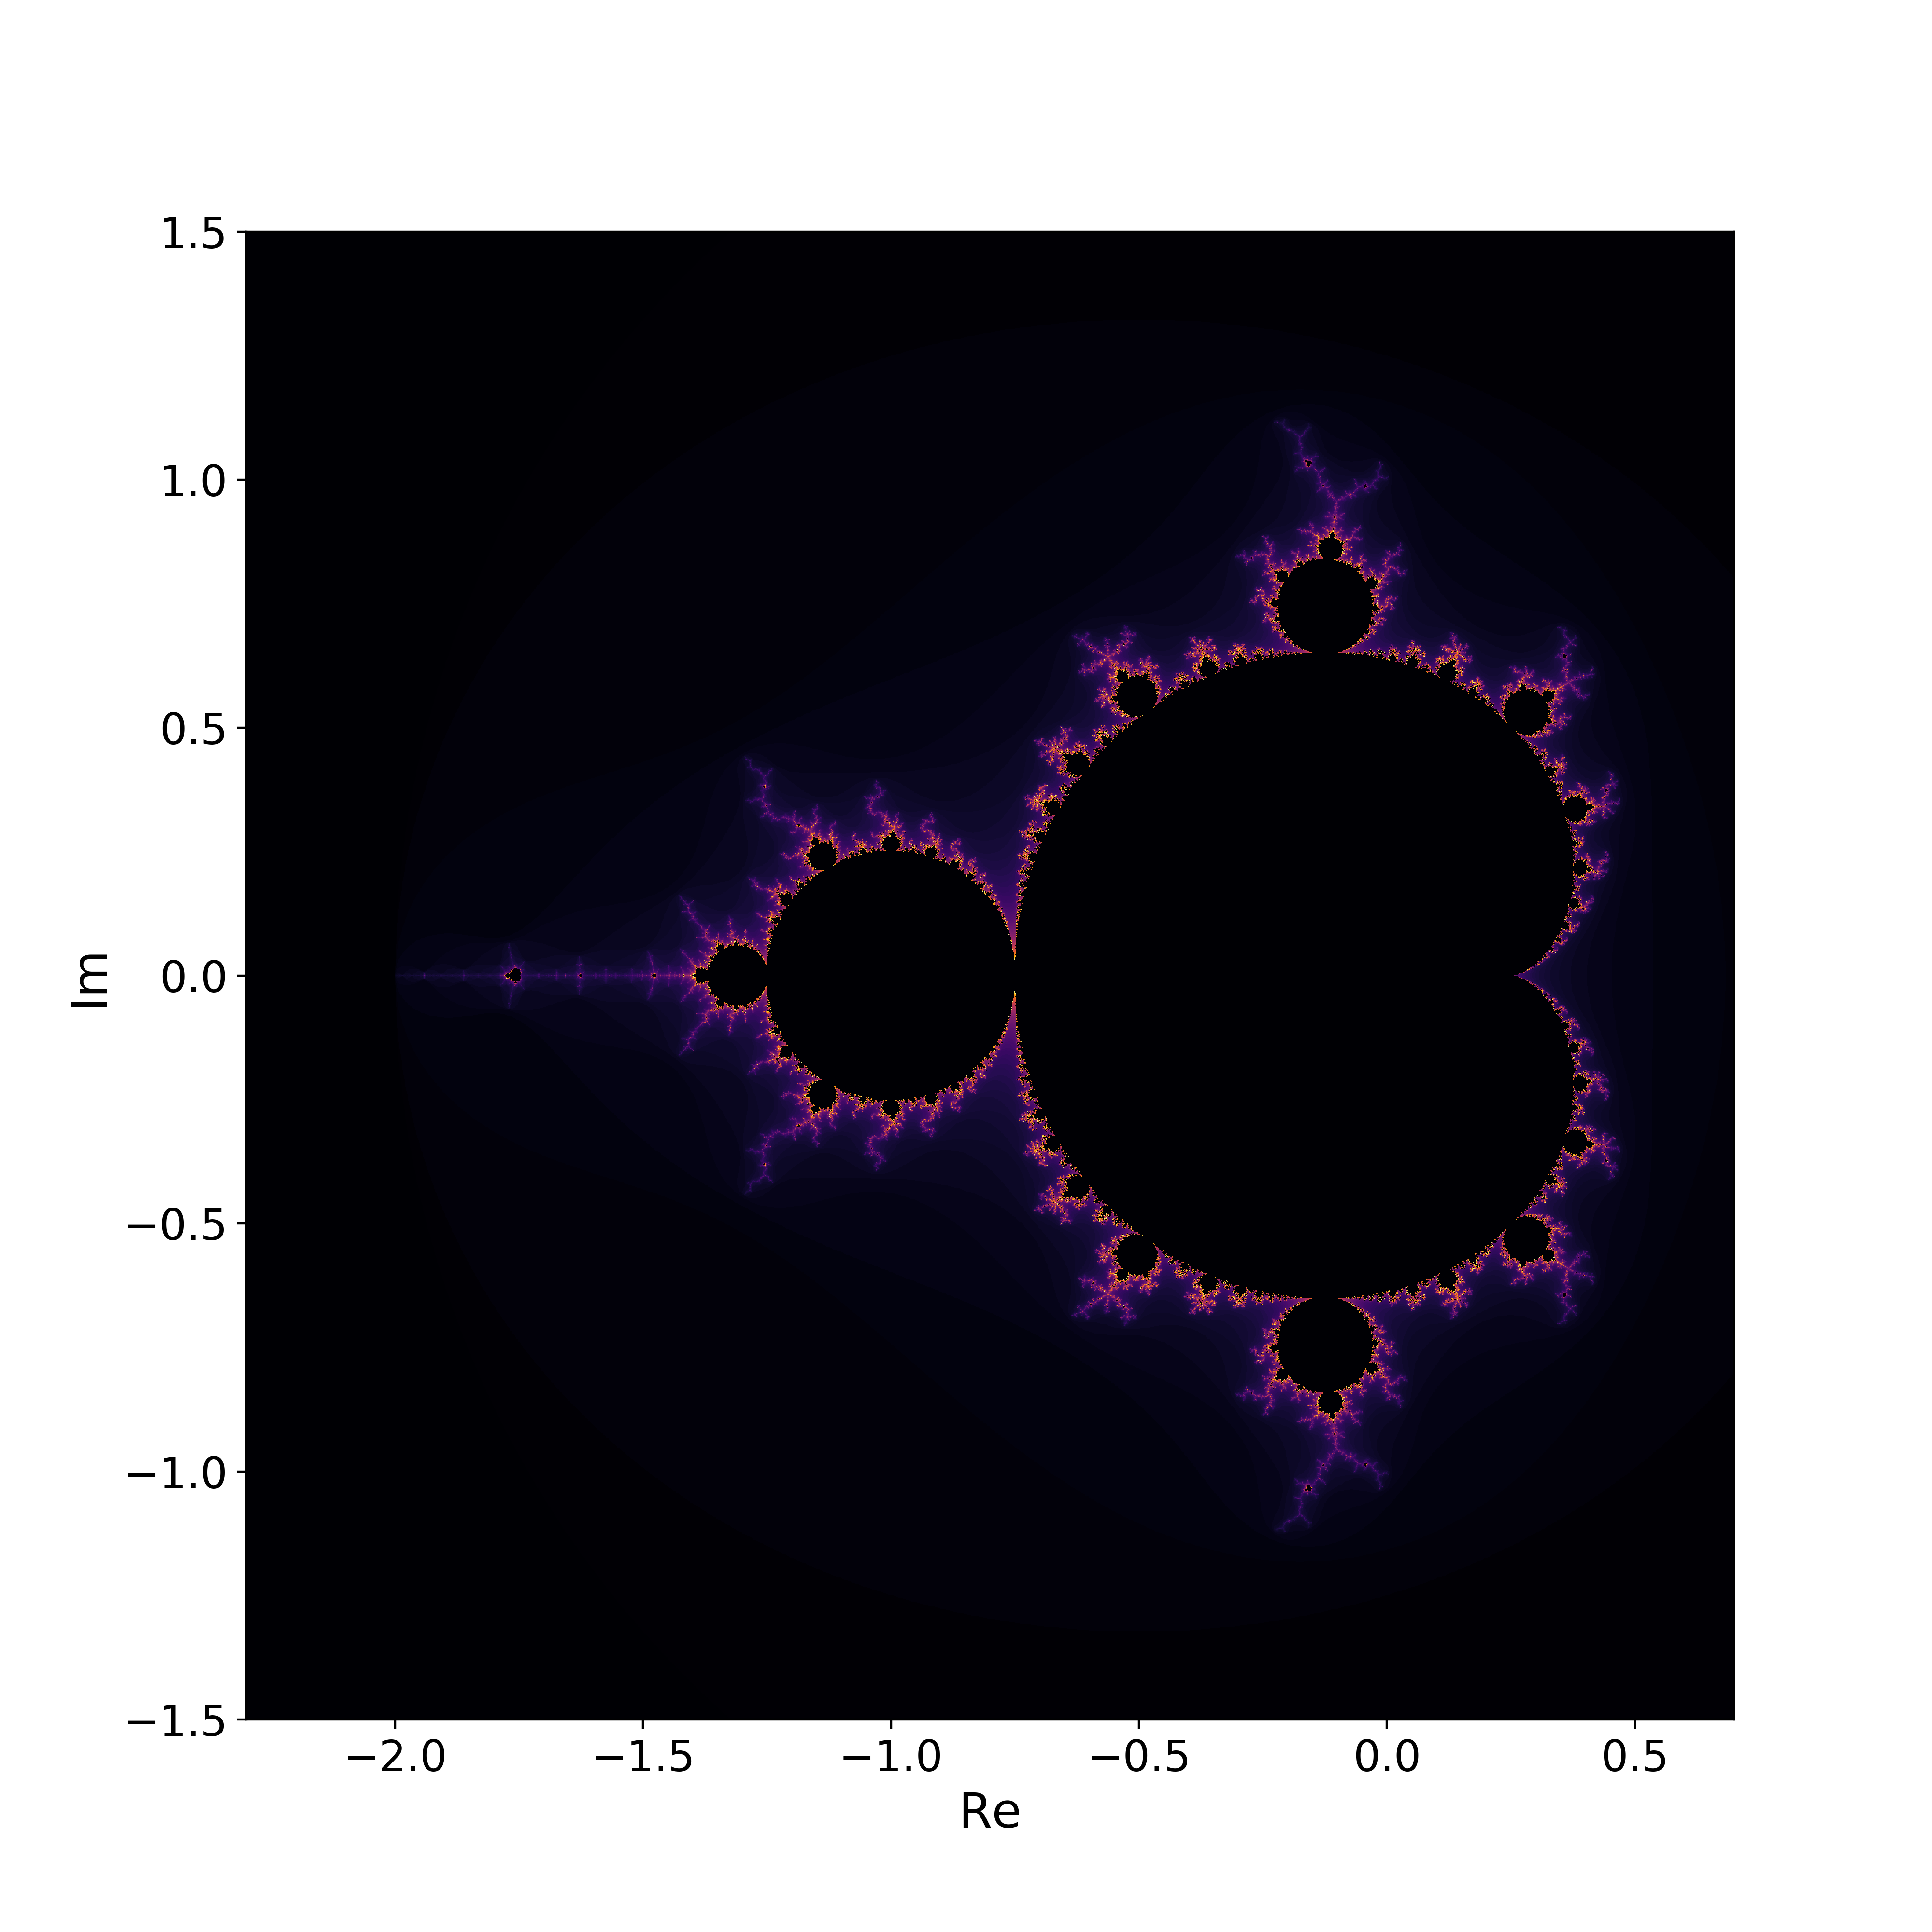
\includegraphics[width=\linewidth]{IMG/Res4.png}
  \caption{Grid Size $2000 \, \times \, 2000$.}
\end{subfigure}
\caption{Variation of the resolution.}
\label{FIG_Resolution}
\end{figure}




\newpage
\subsubsection{Variation of the Number of Iterations}

\begin{figure}[H]
\centering
\begin{subfigure}{.45\textwidth}
  \centering
  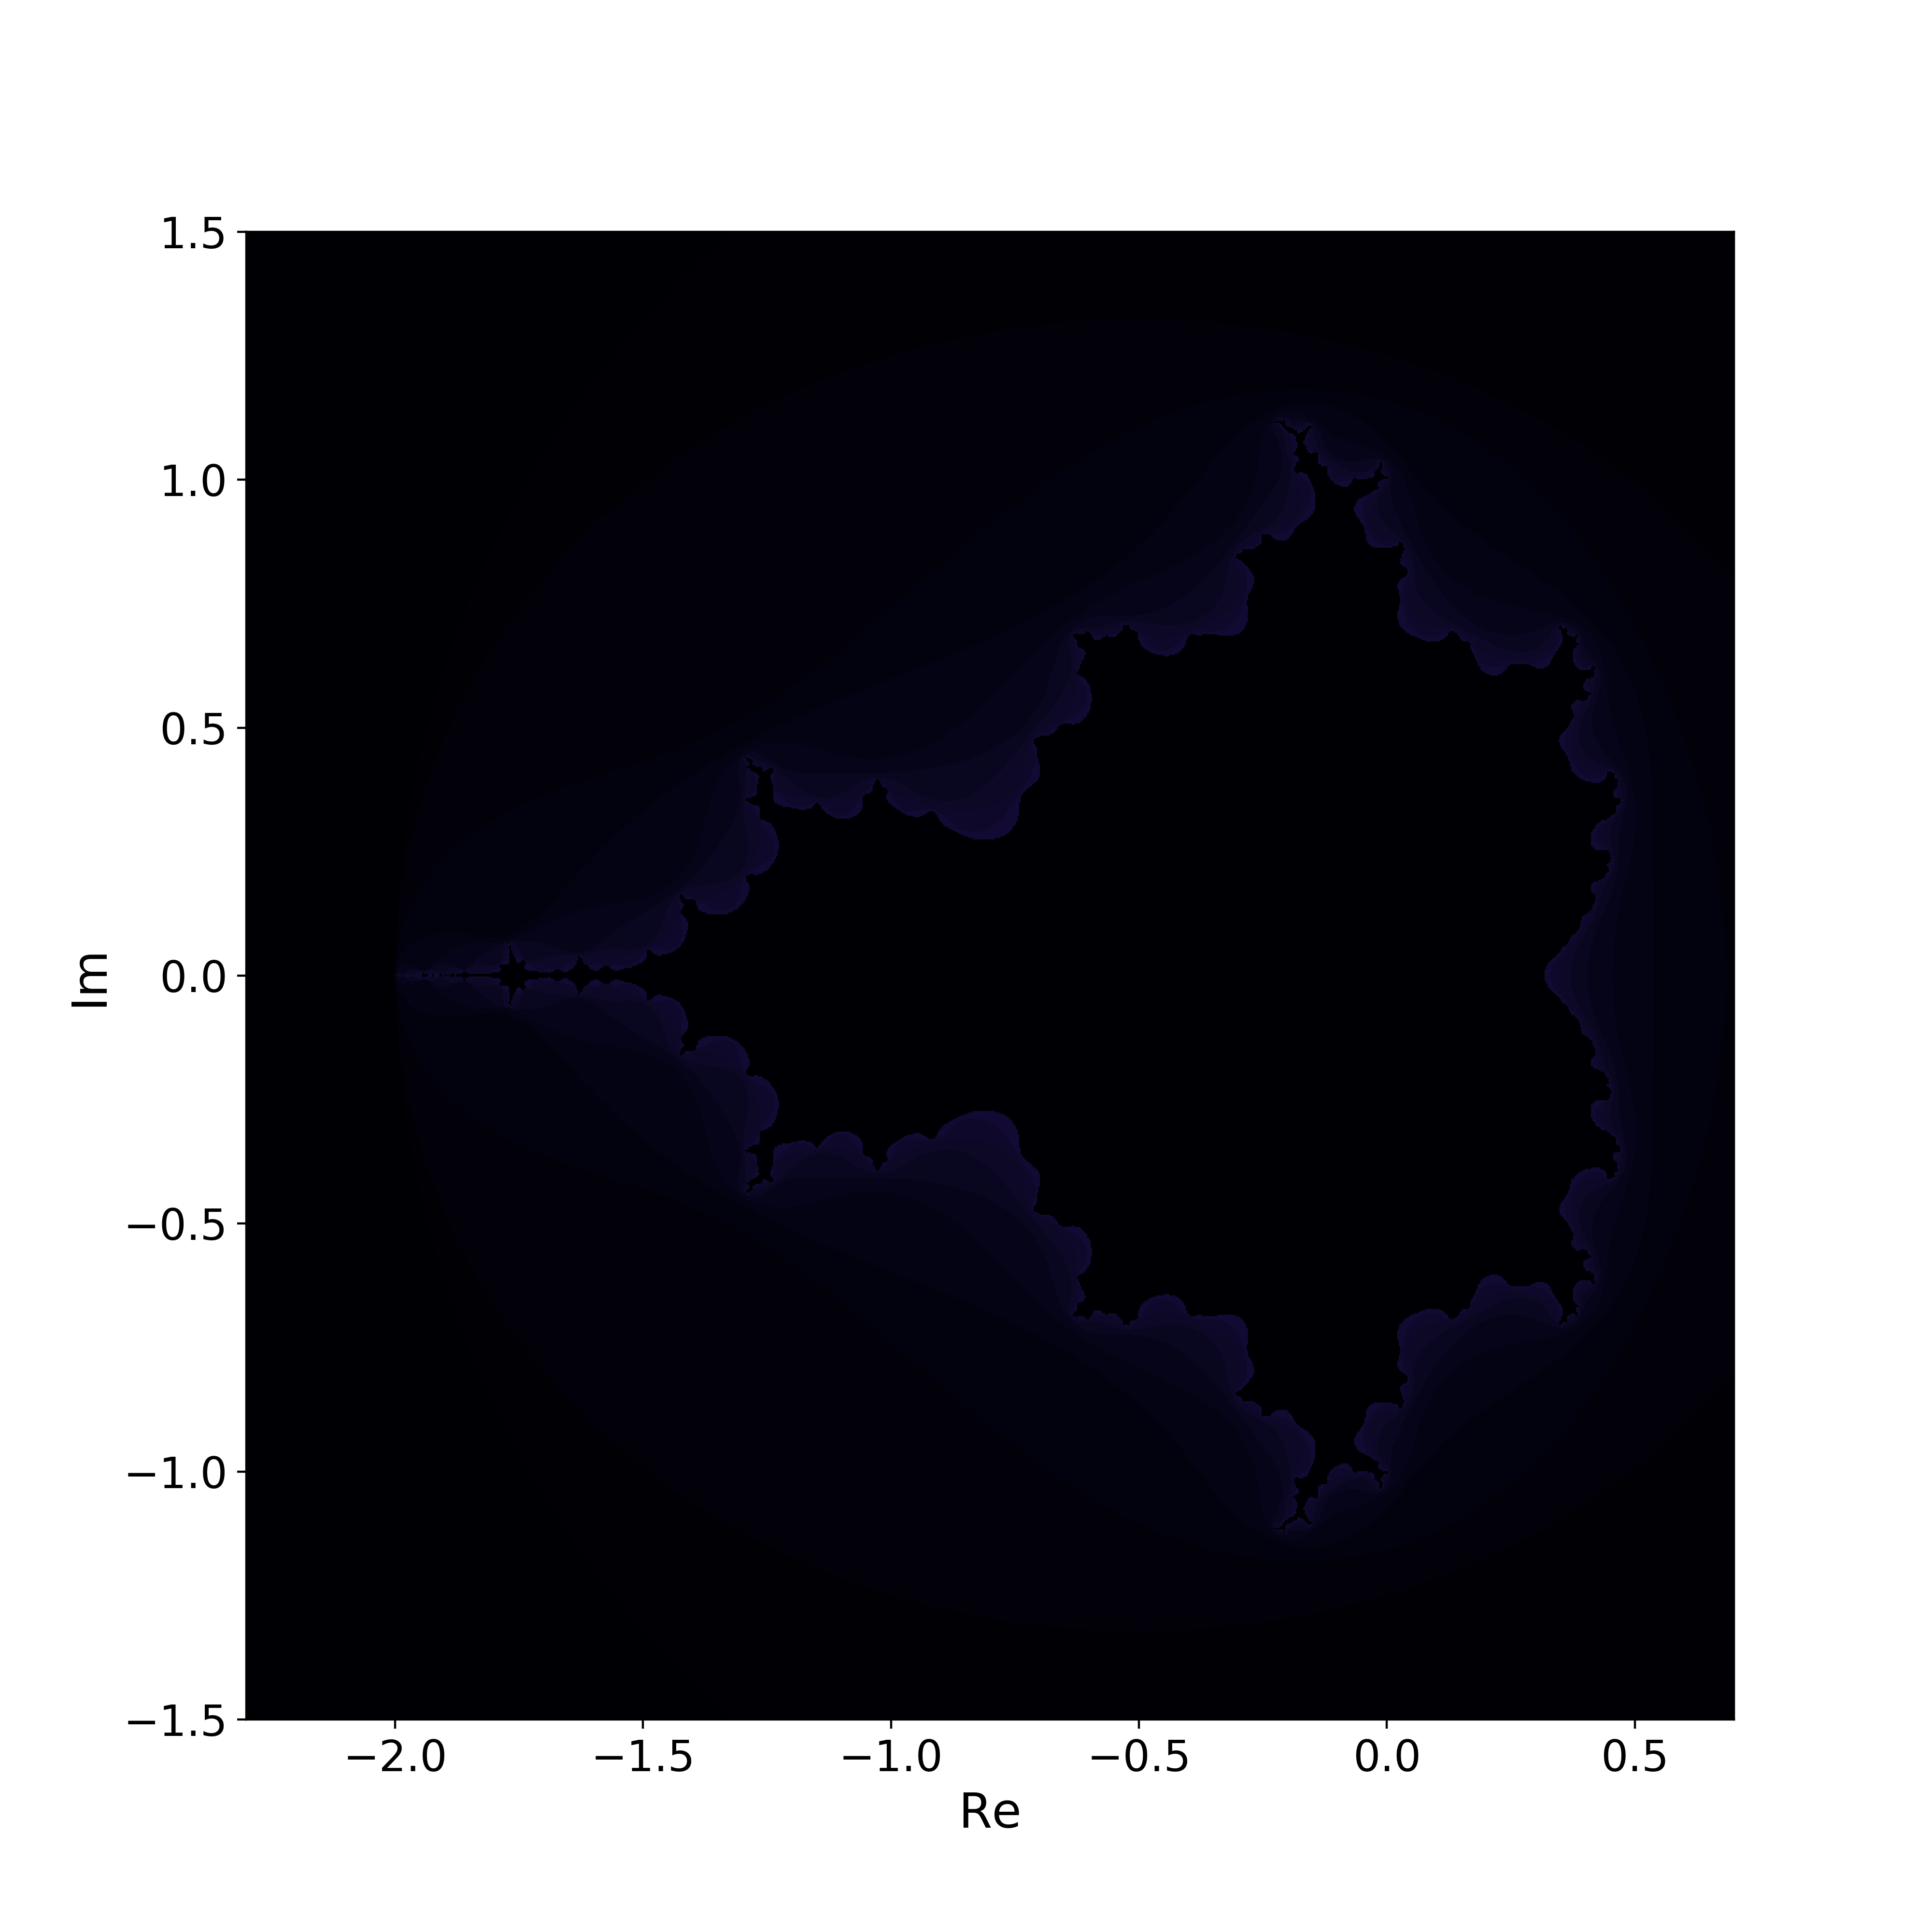
\includegraphics[width=\linewidth]{IMG/It10.png}
  \caption{Ten iterations.}
\end{subfigure}%
\begin{subfigure}{.45\textwidth}
  \centering
  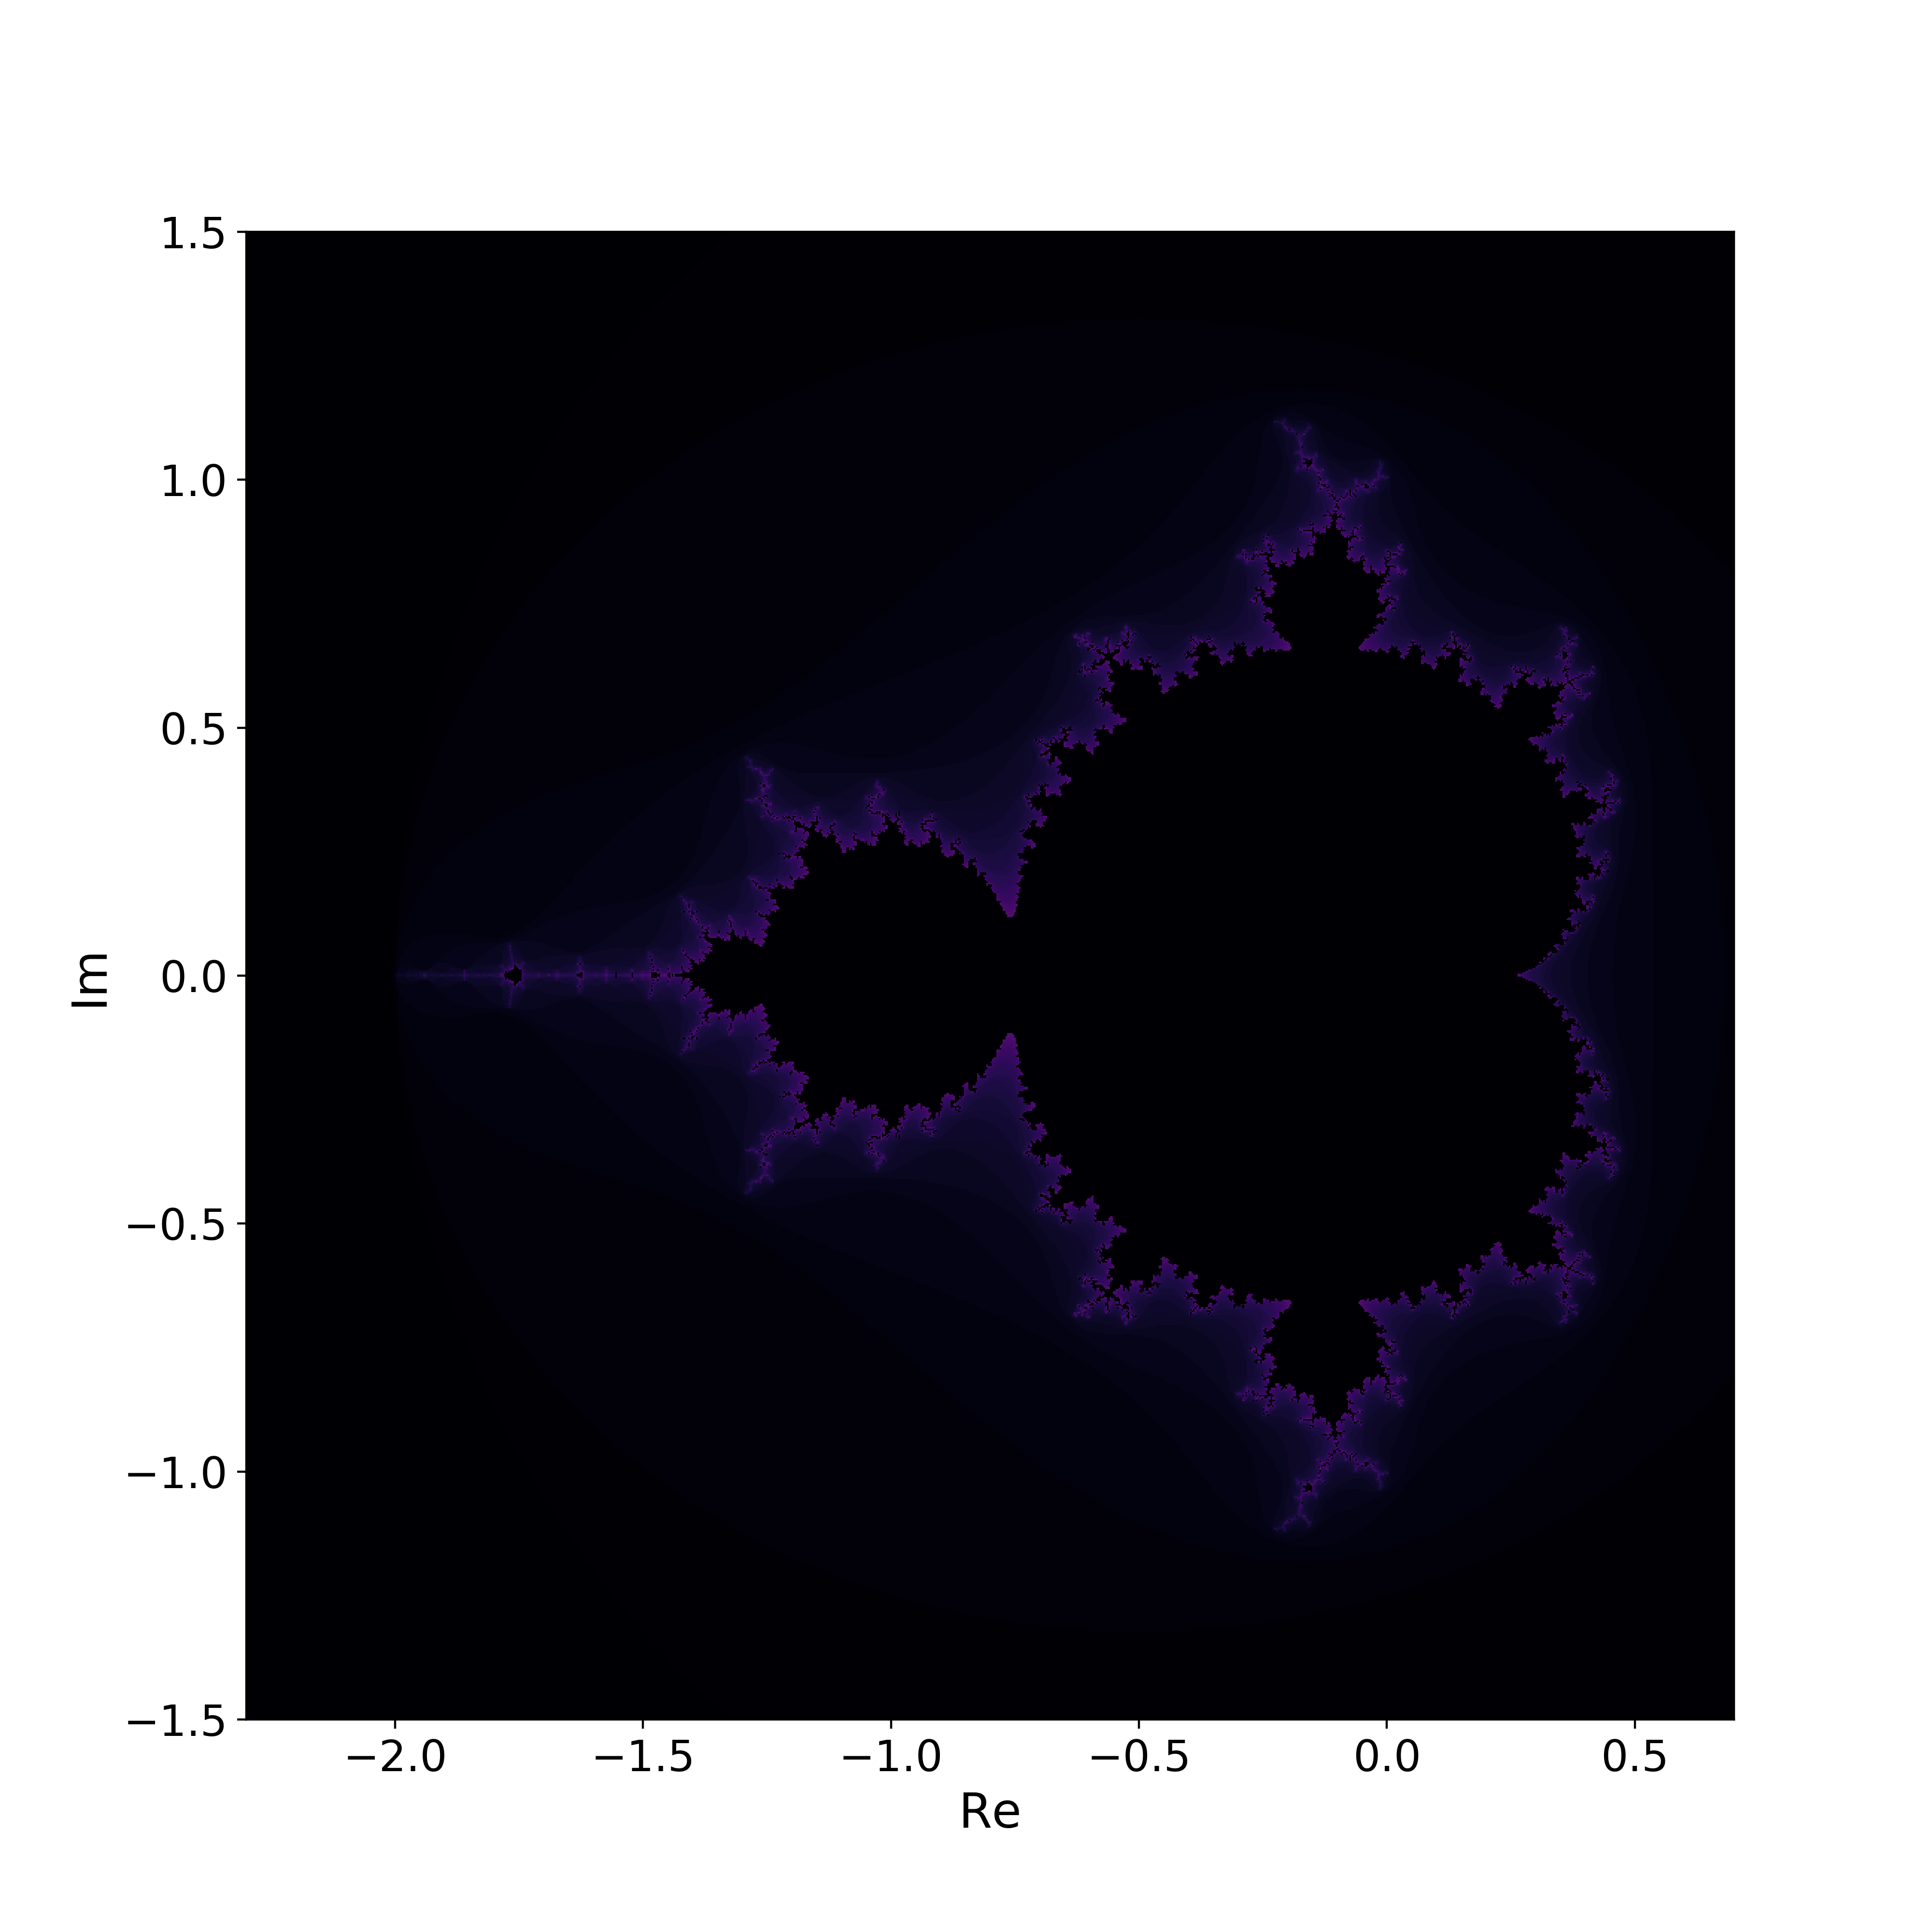
\includegraphics[width=\linewidth]{IMG/It25.png}
  \caption{25 iterations.}
\end{subfigure}
\begin{subfigure}{.45\textwidth}
  \centering
  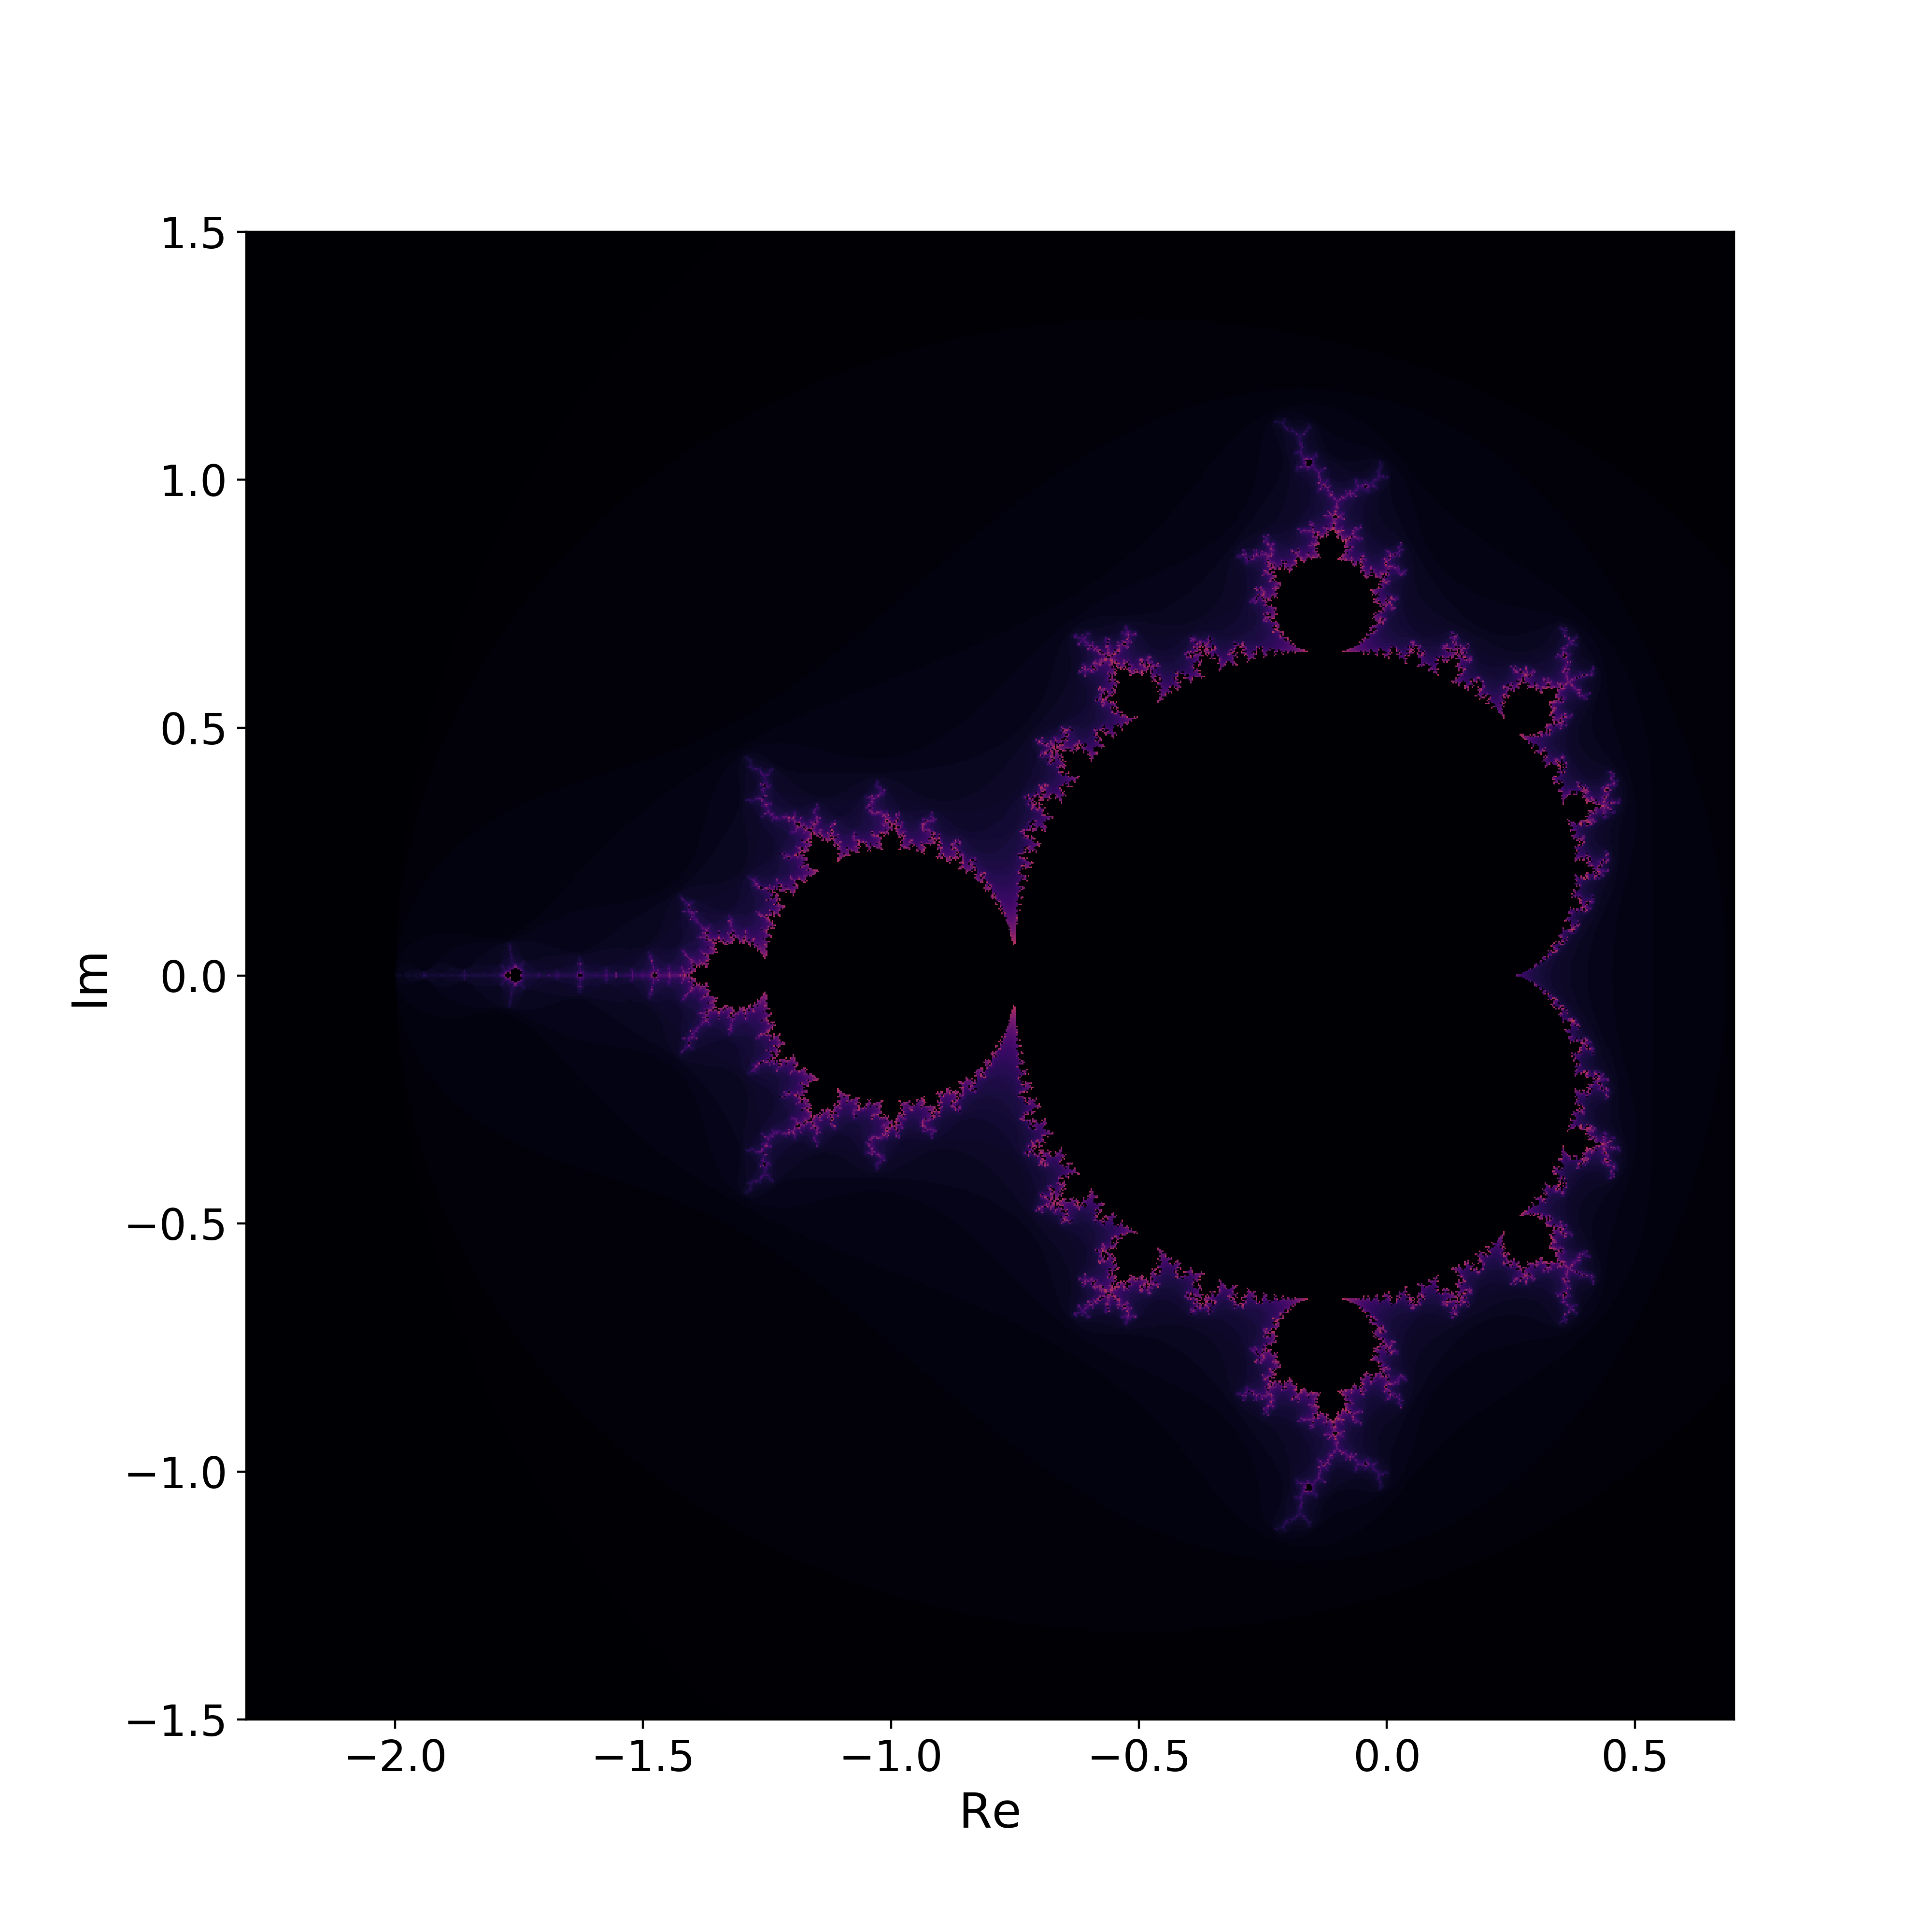
\includegraphics[width=\linewidth]{IMG/It50.png}
  \caption{50 iterations.}
\end{subfigure}
\begin{subfigure}{.45\textwidth}
  \centering
  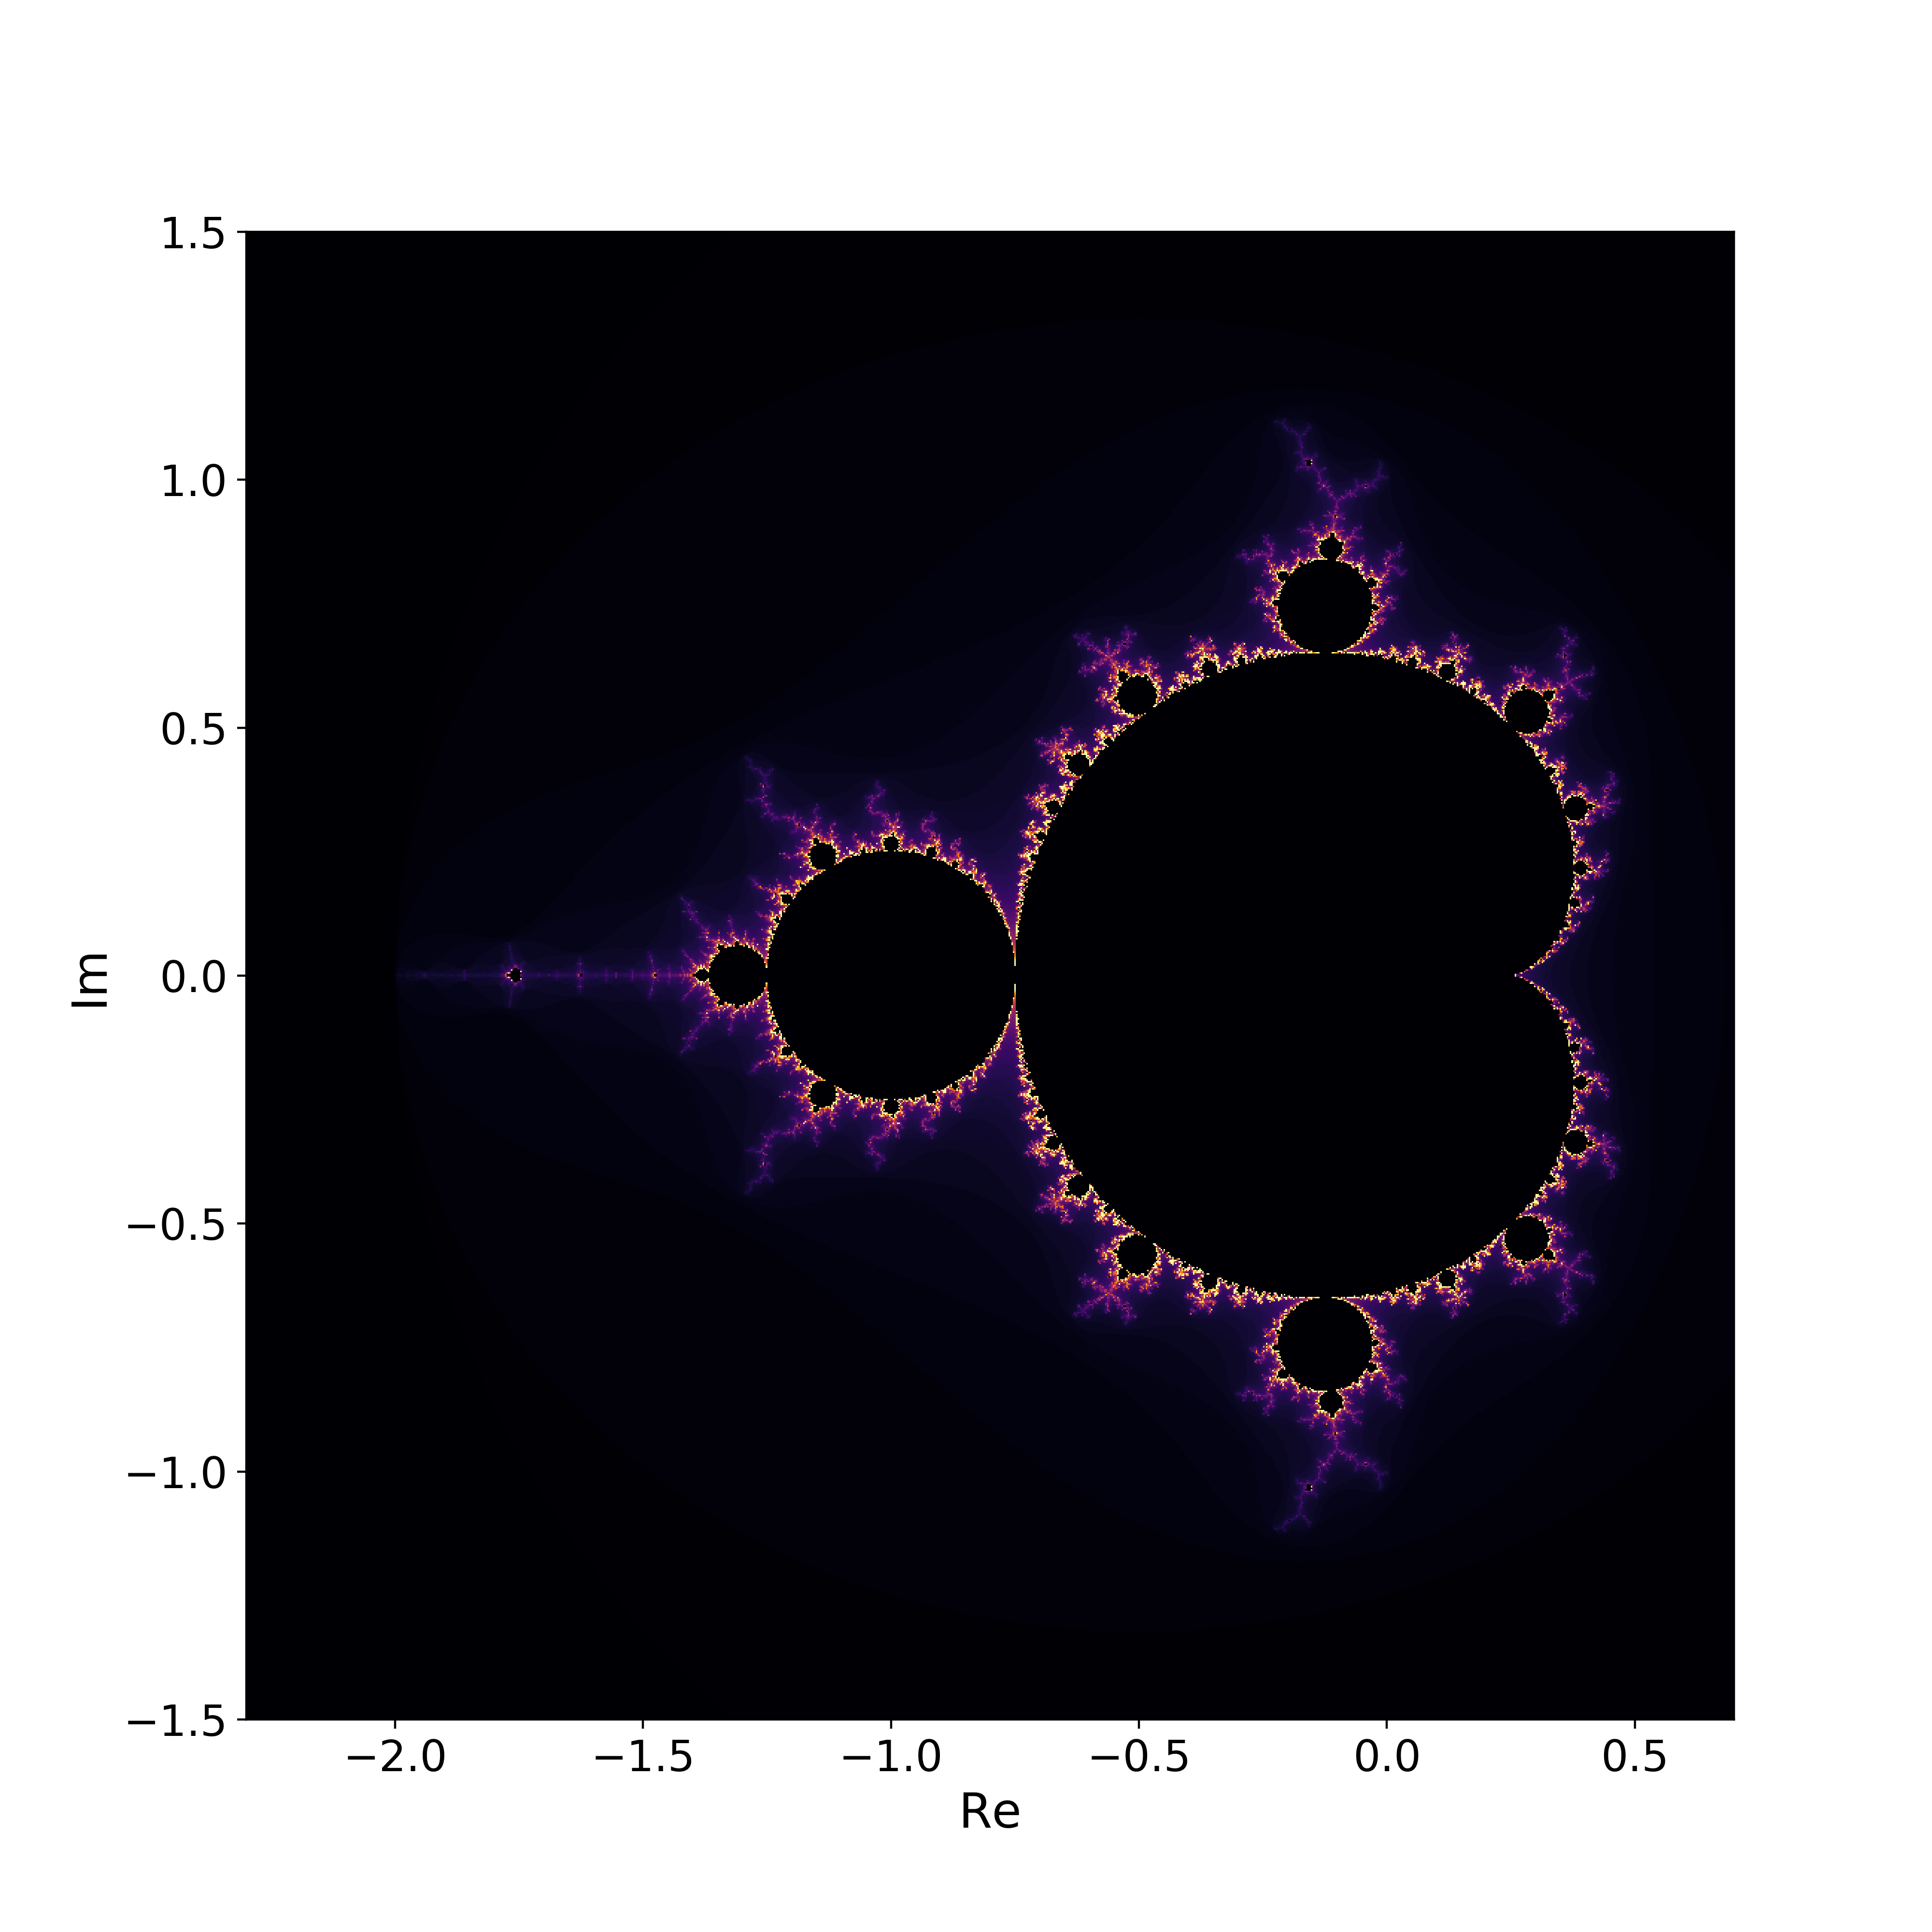
\includegraphics[width=\linewidth]{IMG/It500.png}
  \caption{500 iterations.}
\end{subfigure}
\caption{Variation of the number of iterations.}
\label{FIG_Iteration}
\end{figure}



\newpage
\subsubsection{Variation of the Threshold Value}

\begin{figure}[H]
\centering
\begin{subfigure}{.45\textwidth}
  \centering
  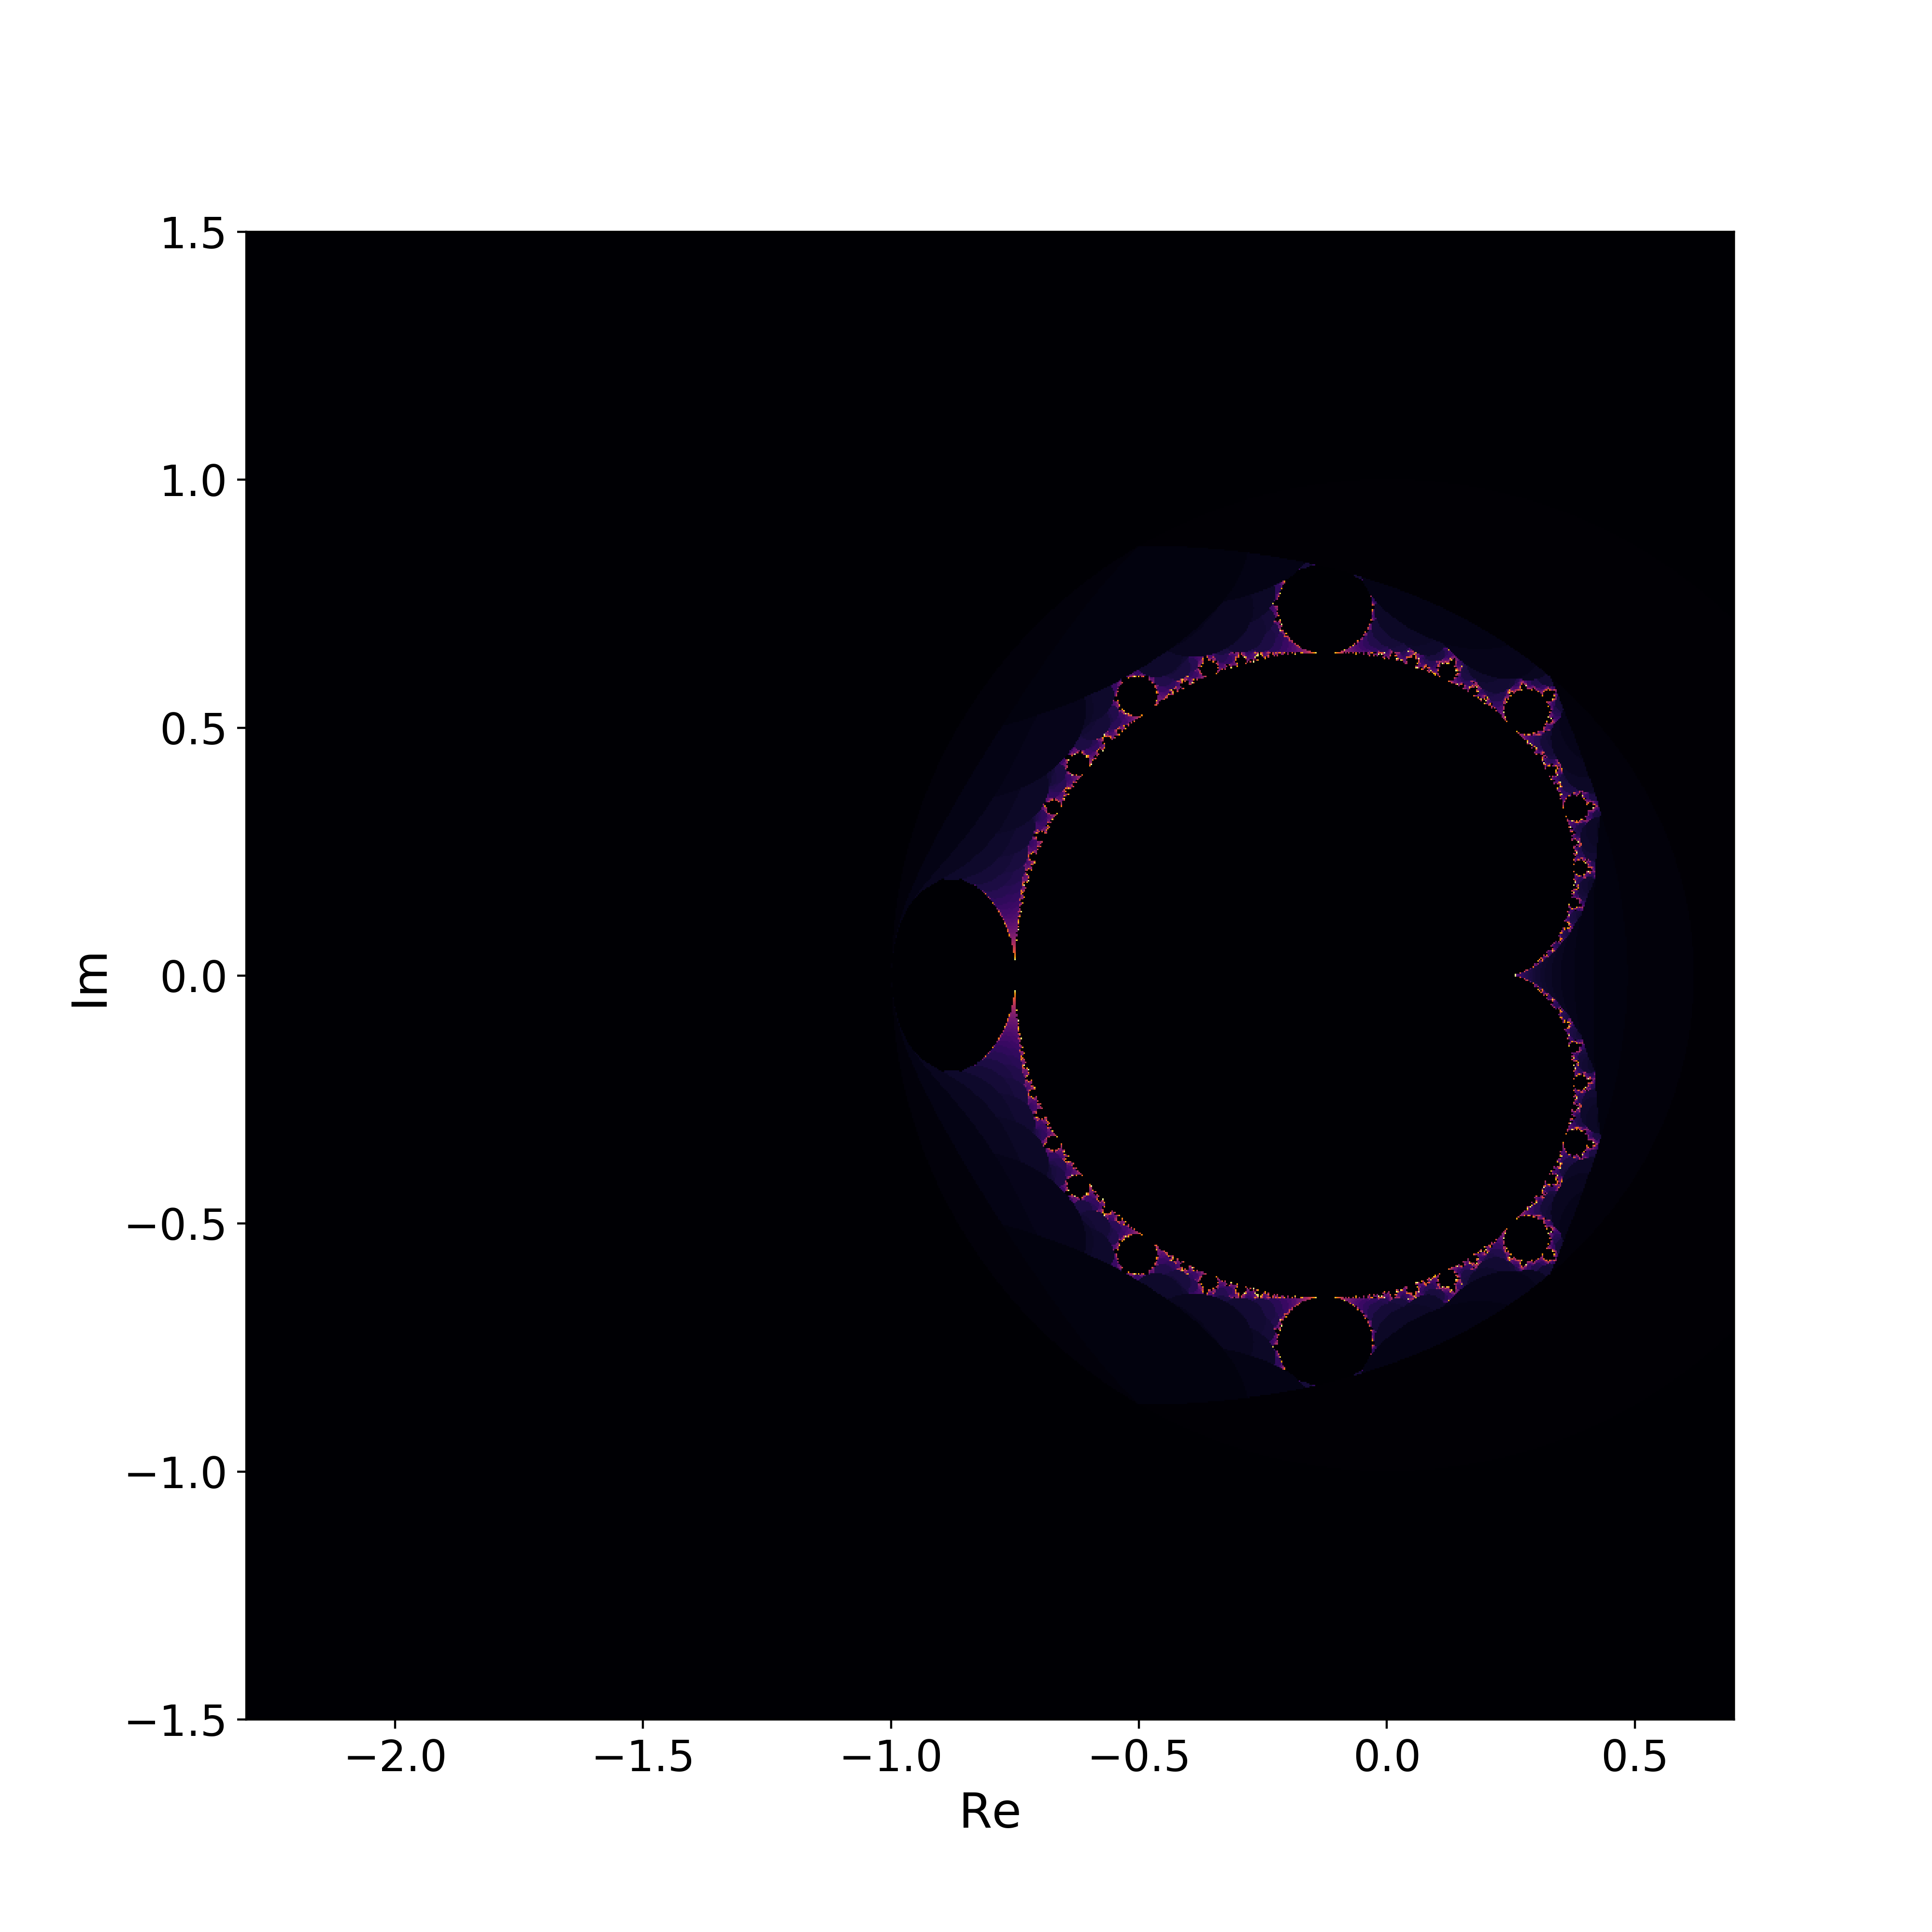
\includegraphics[width=\linewidth]{IMG/Thresh05.png}
  \caption{Threshold of $0.5$.}
\end{subfigure}%
\begin{subfigure}{.45\textwidth}
  \centering
  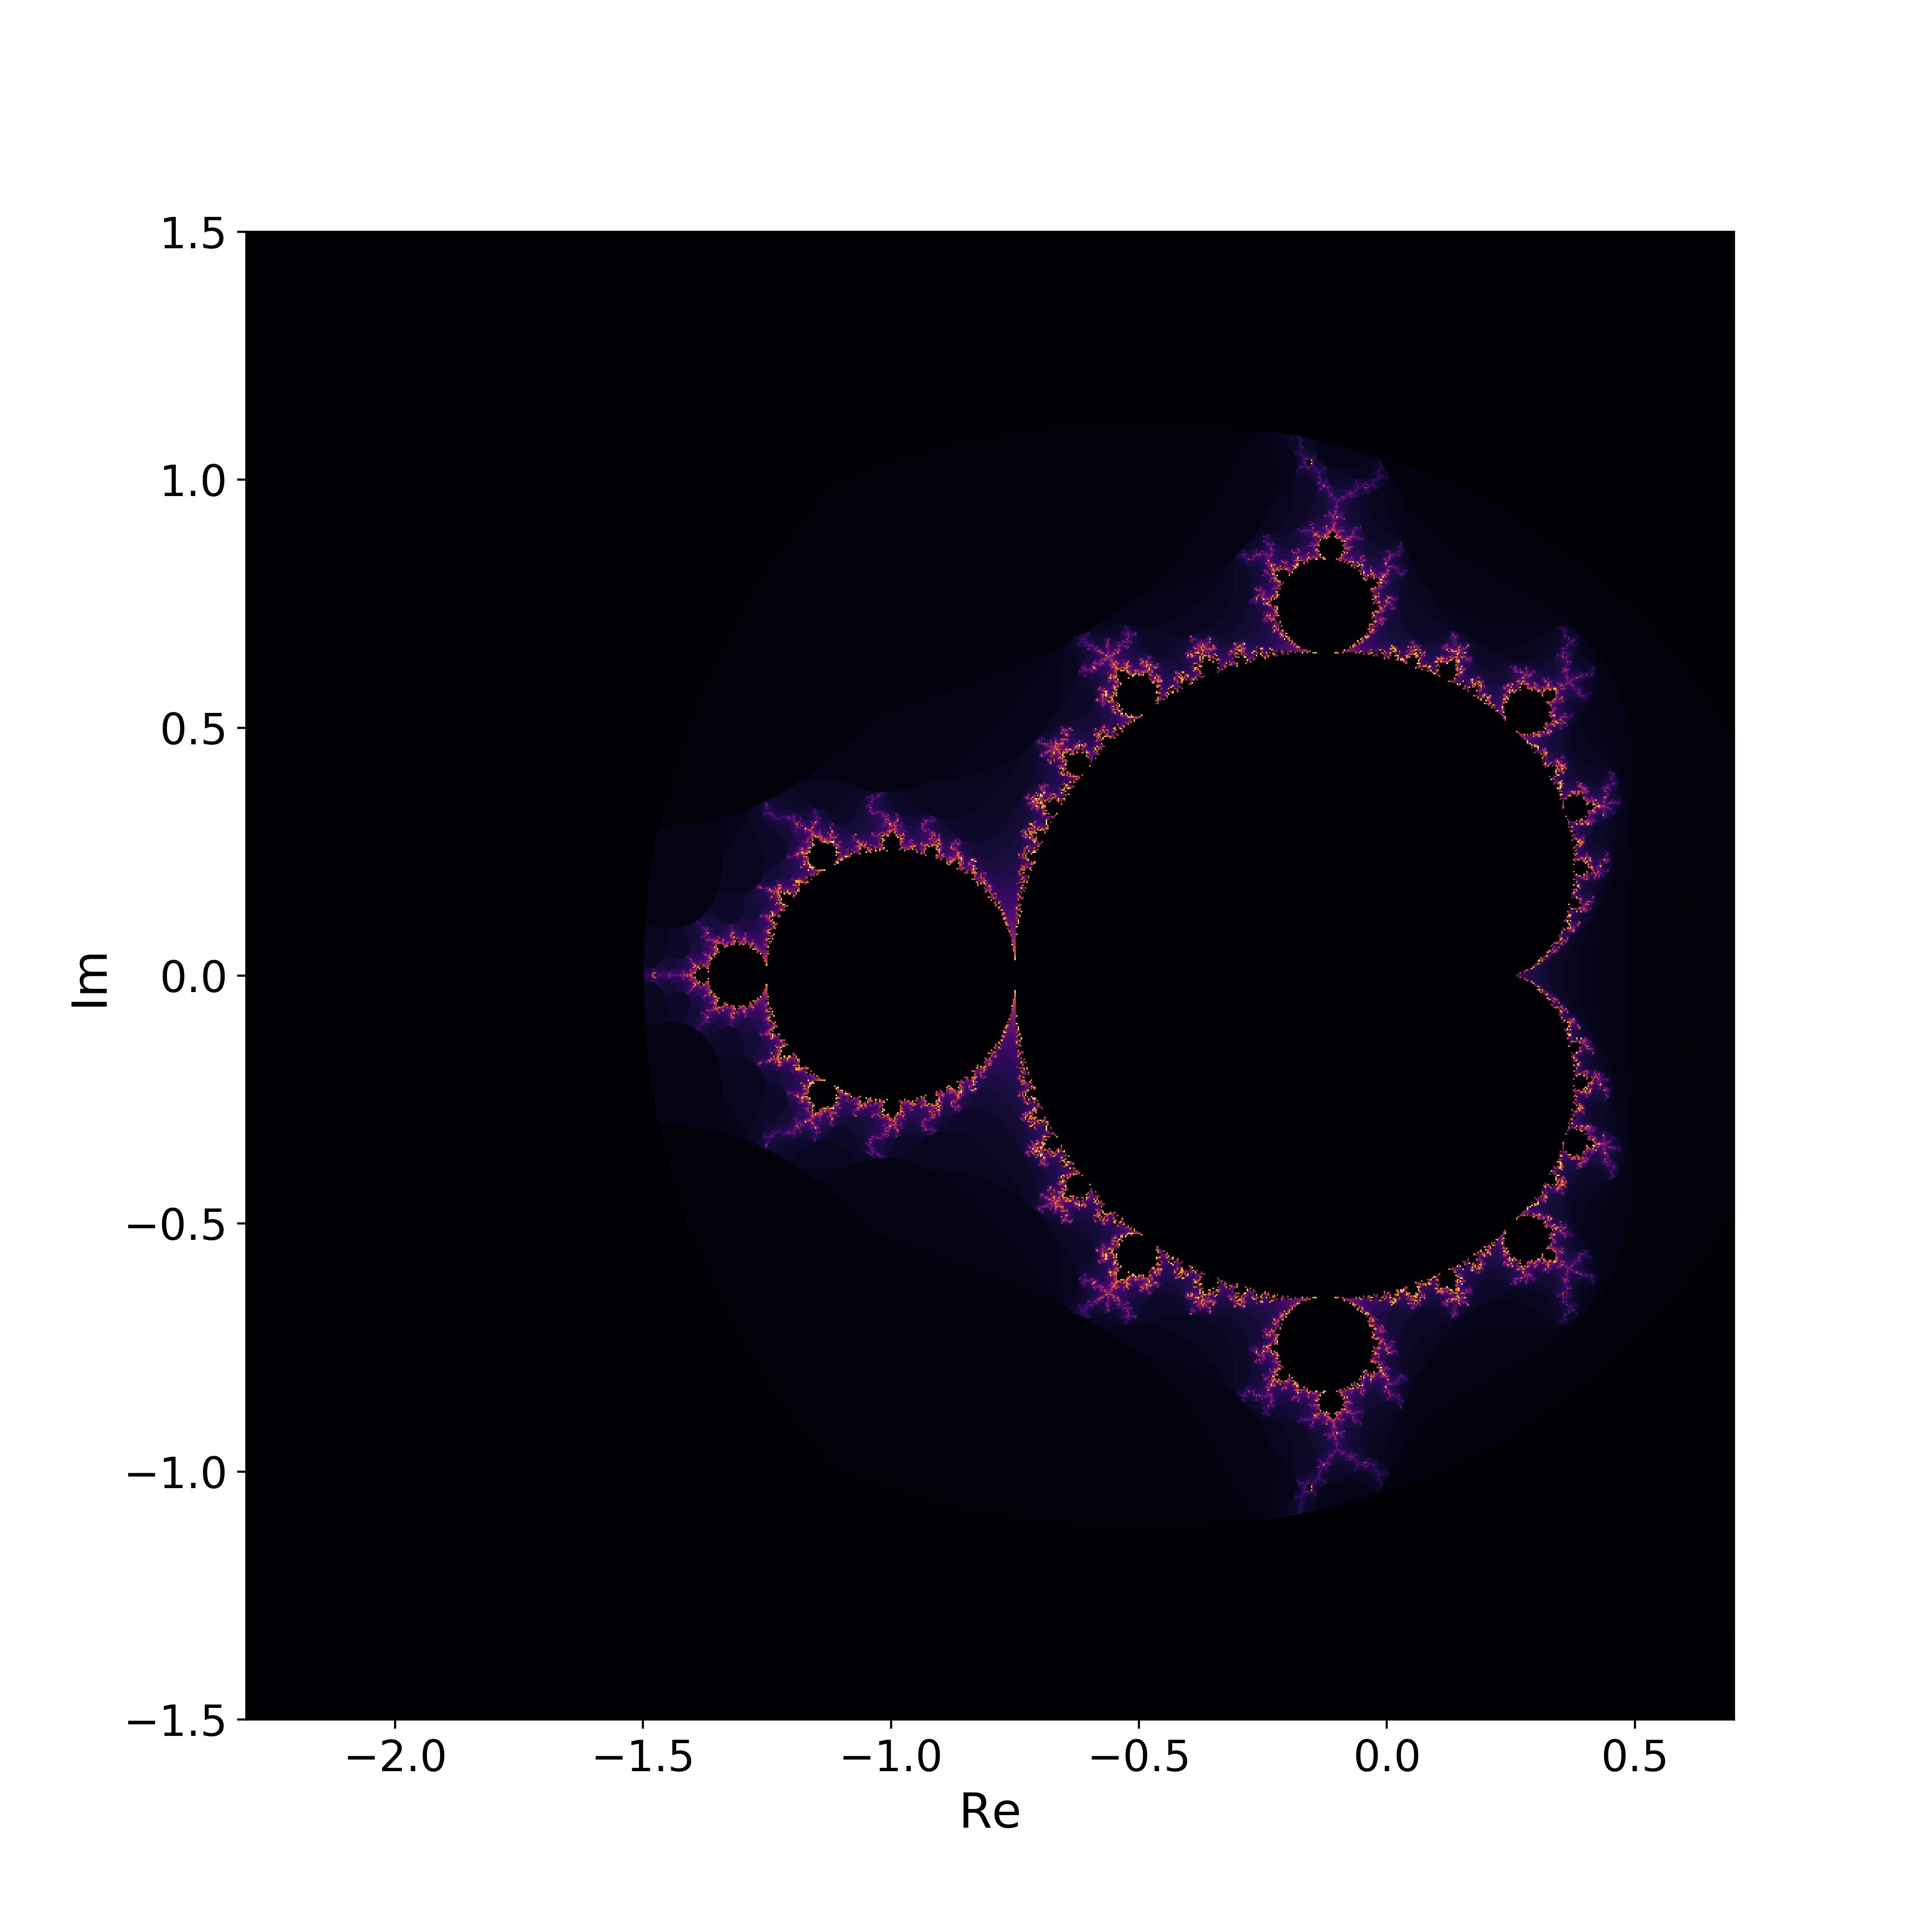
\includegraphics[width=\linewidth]{IMG/Thresh1.png}
  \caption{Threshold of $1.0$.}
\end{subfigure}
\begin{subfigure}{.45\textwidth}
  \centering
  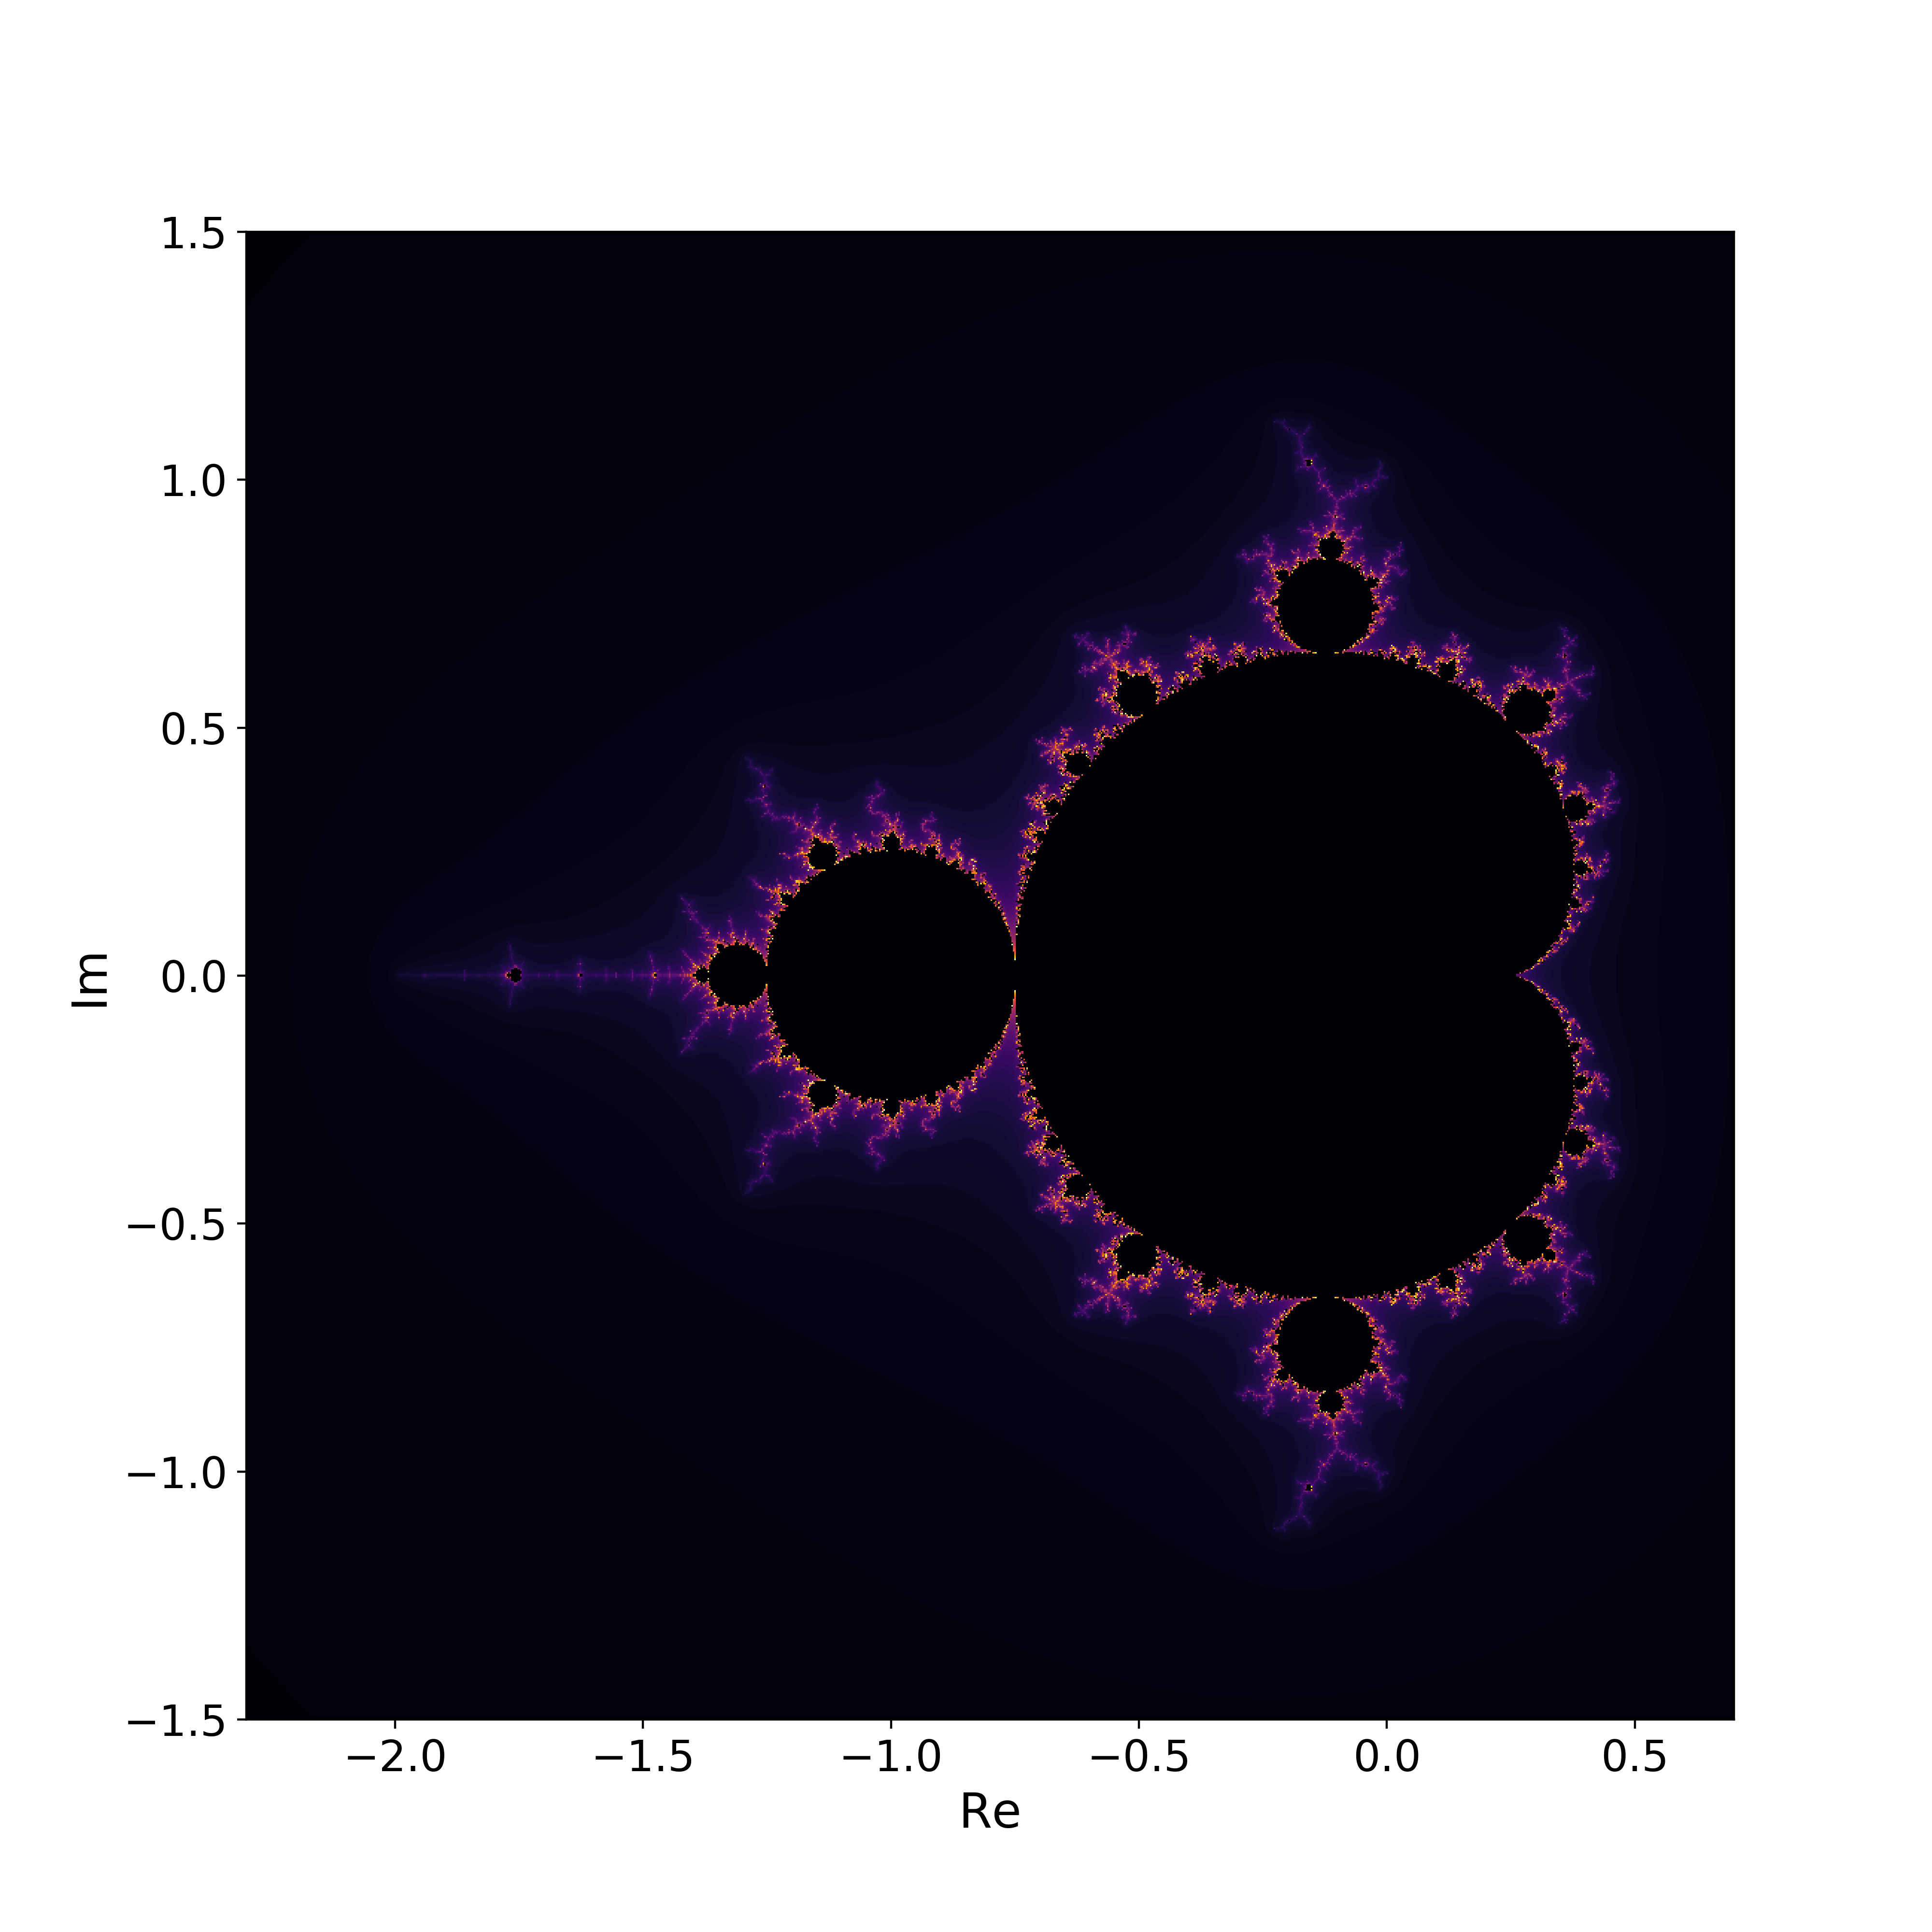
\includegraphics[width=\linewidth]{IMG/Thresh5.png}
  \caption{Threshold of $5.0$.}
\end{subfigure}
\begin{subfigure}{.45\textwidth}
  \centering
  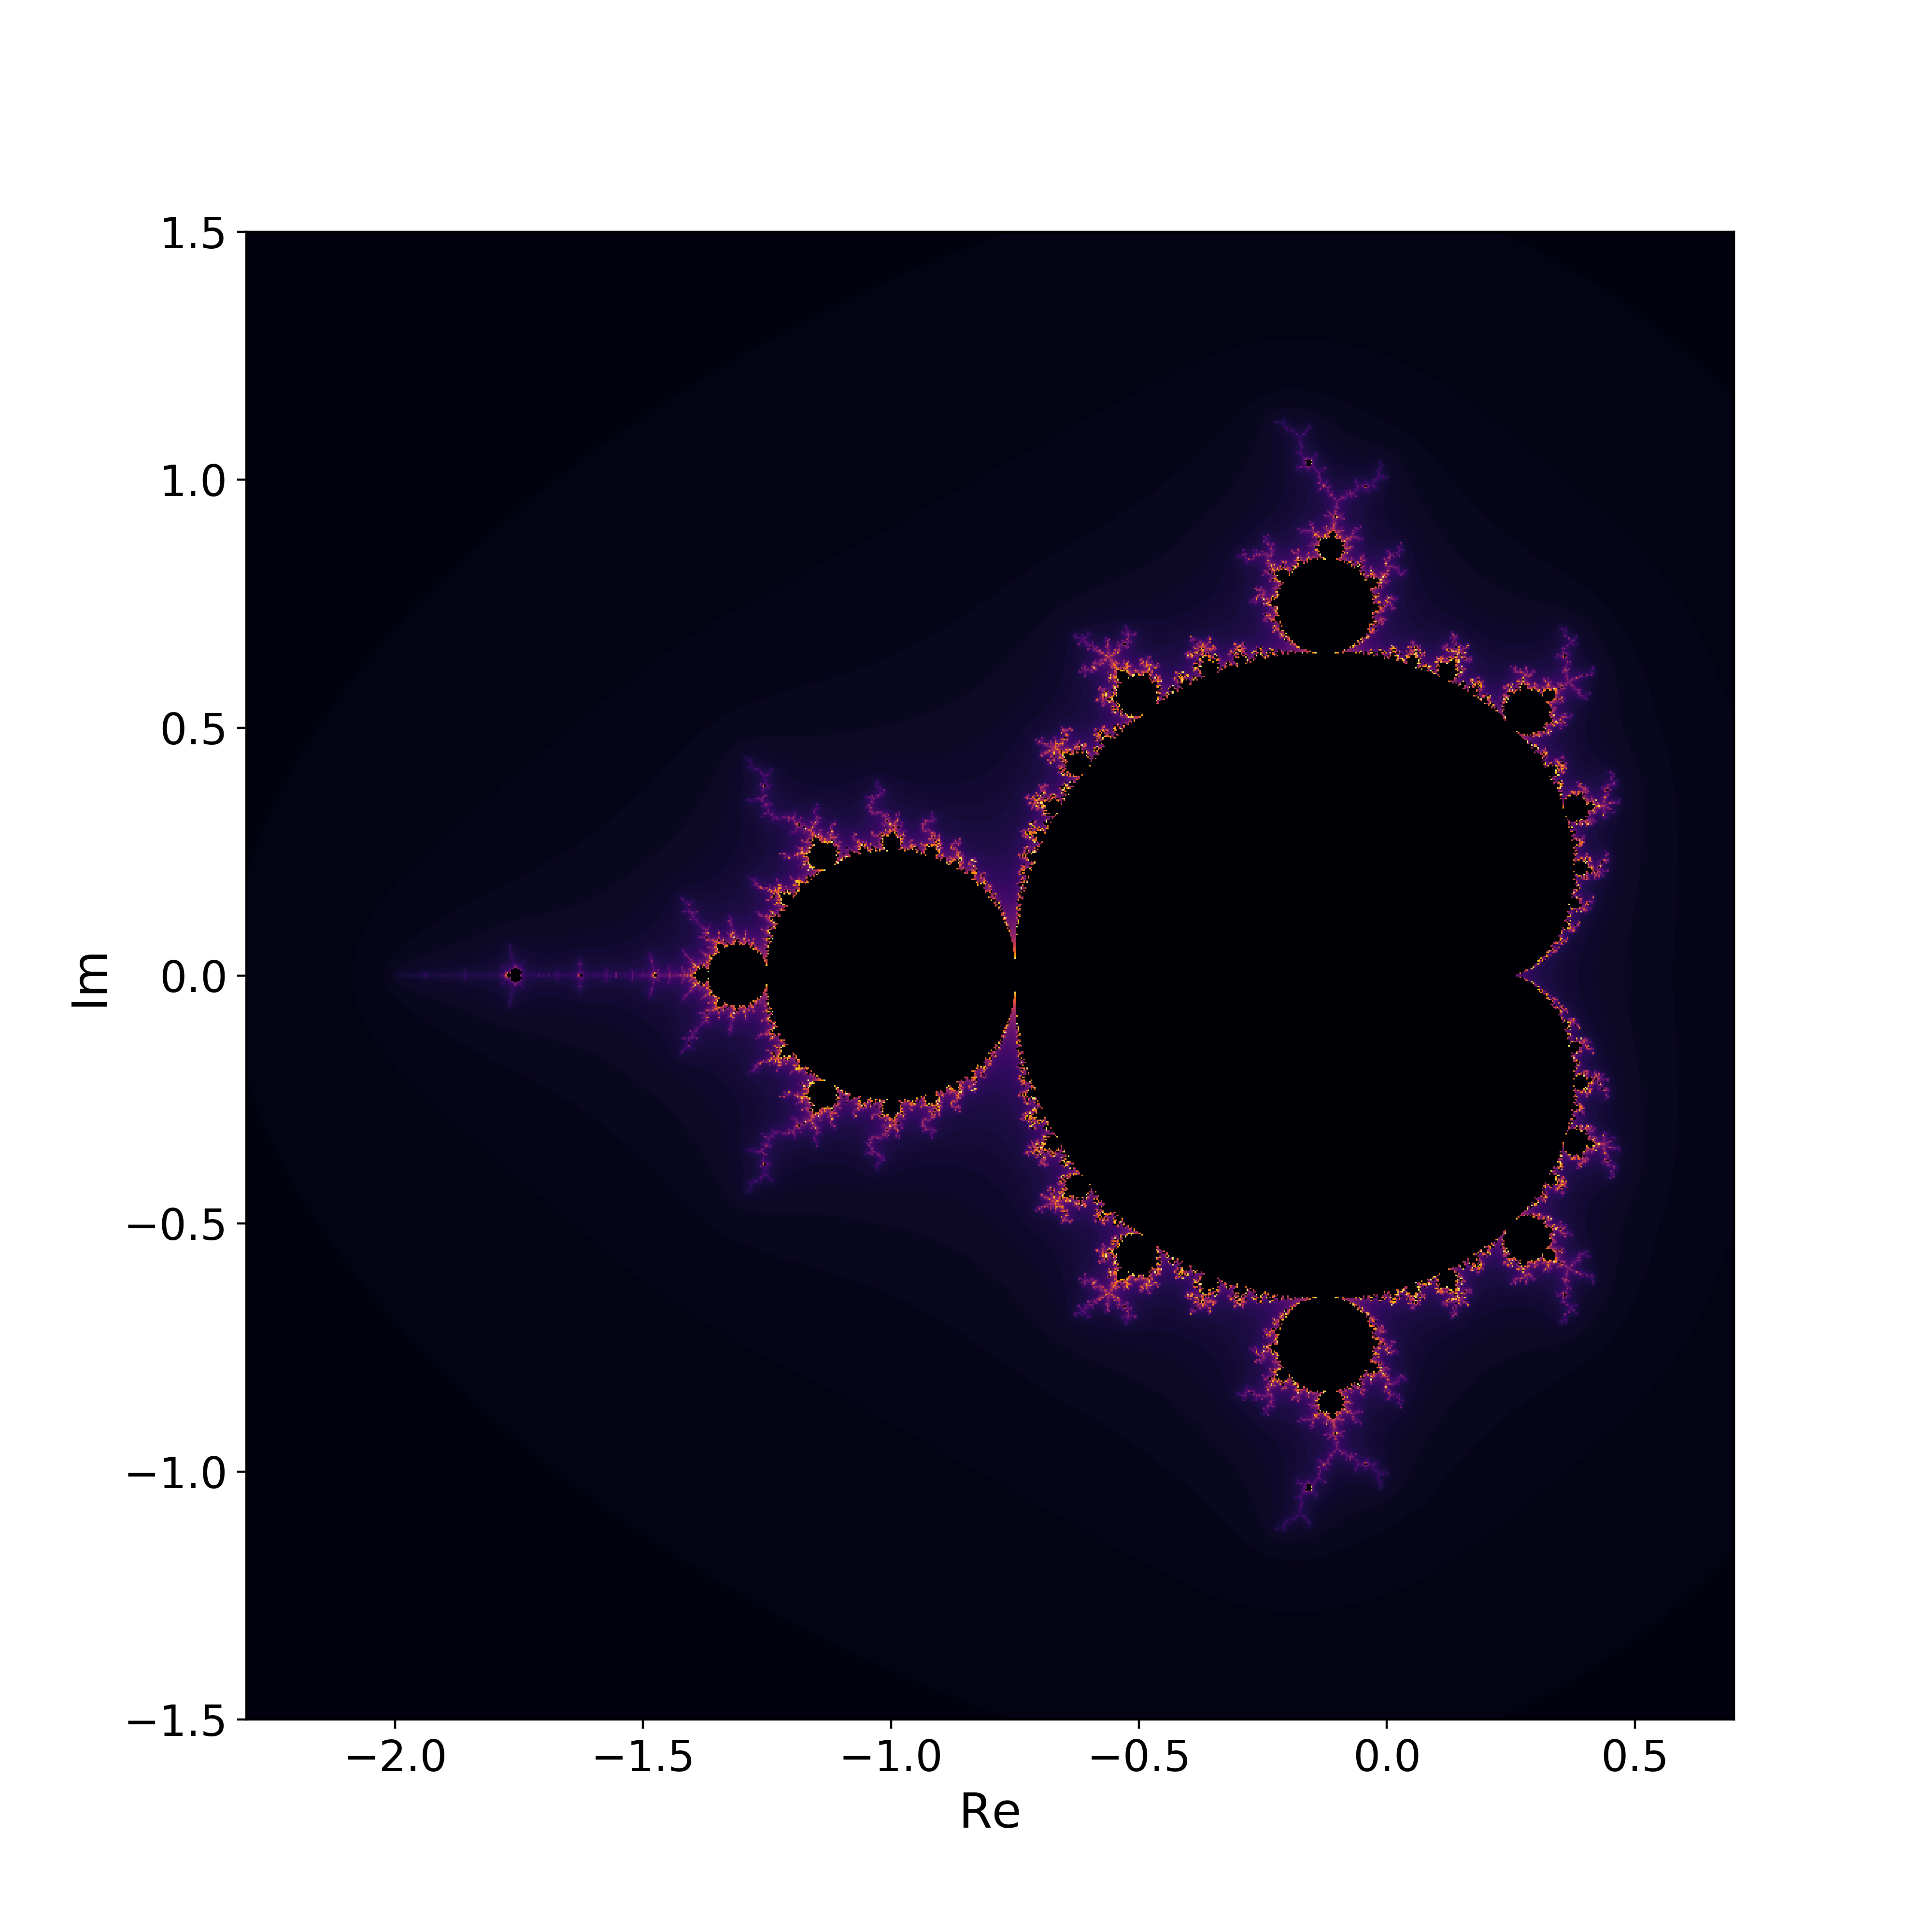
\includegraphics[width=\linewidth]{IMG/Thresh50.png}
  \caption{Threshold of $50.0$.}
\end{subfigure}
\caption{Variation of the threshold value.}
\label{FIG_Threshold}
\end{figure}




\newpage
\subsubsection{Variation of the Coulourmap}

\begin{figure}[H]
\centering
\begin{subfigure}{.45\textwidth}
  \centering
  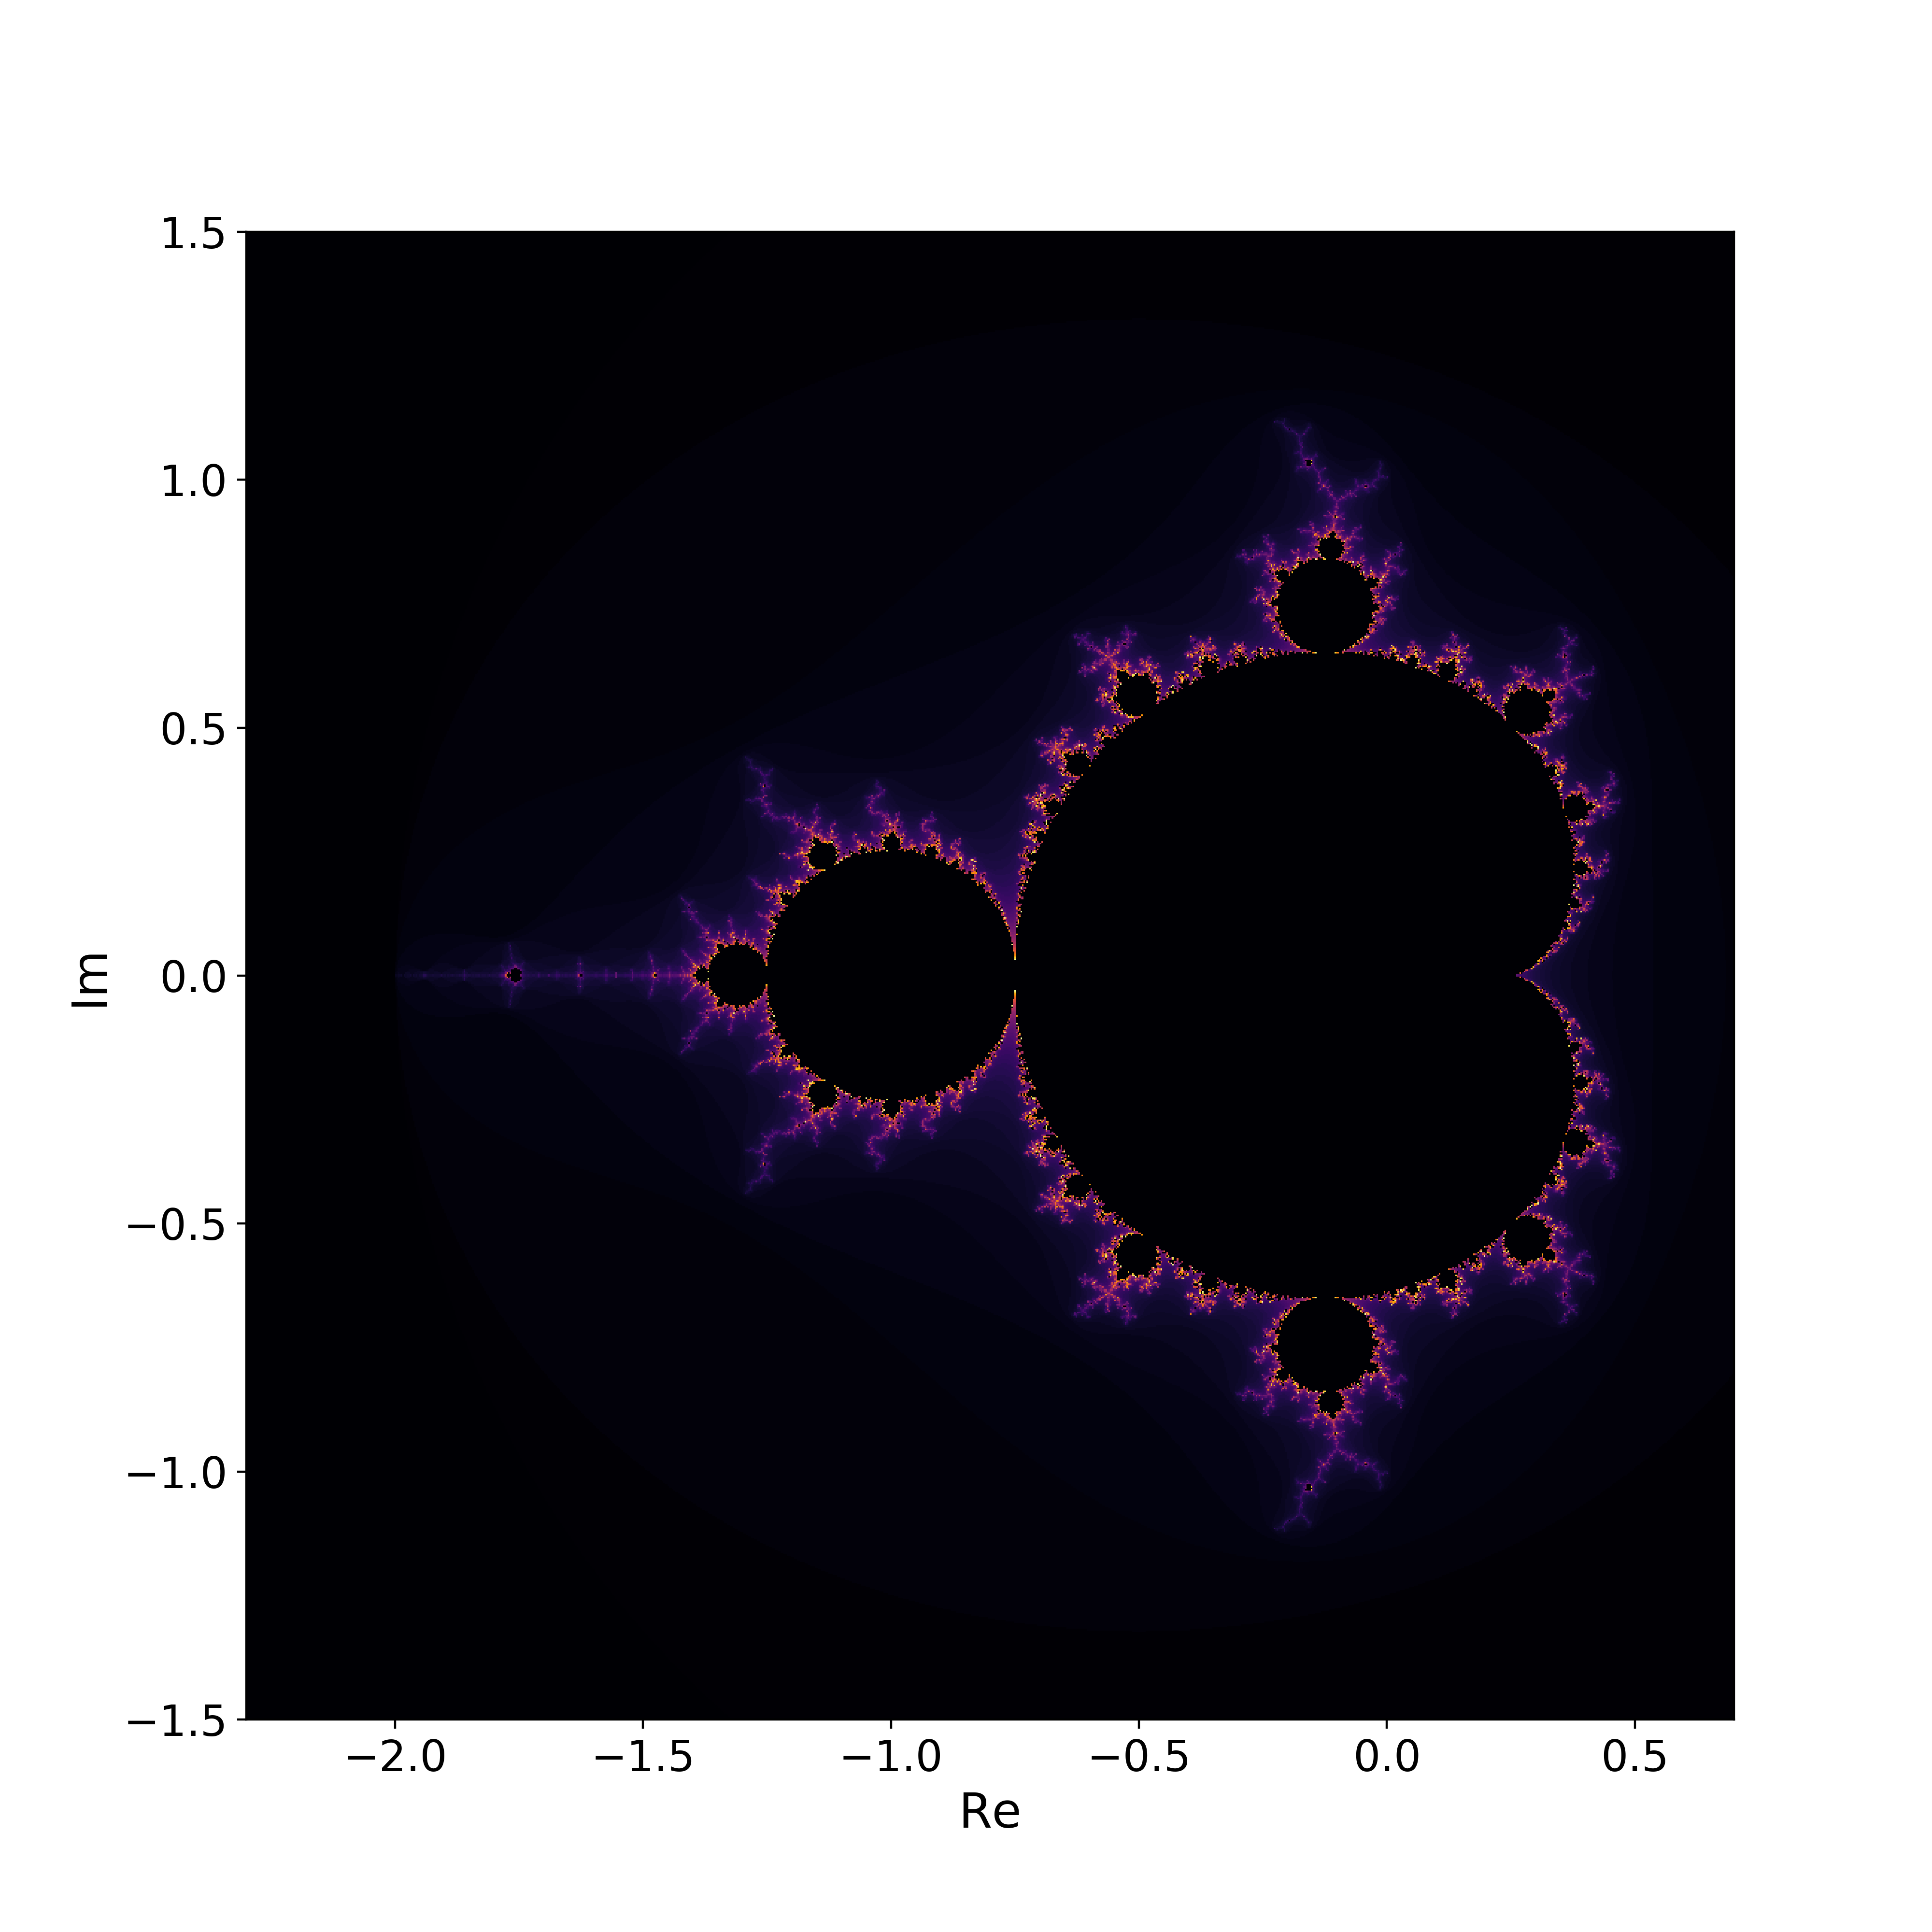
\includegraphics[width=\linewidth]{IMG/ColourInferno.png}
  \caption{{\code{Inferno}} colour map.}
\end{subfigure}%
\begin{subfigure}{.45\textwidth}
  \centering
  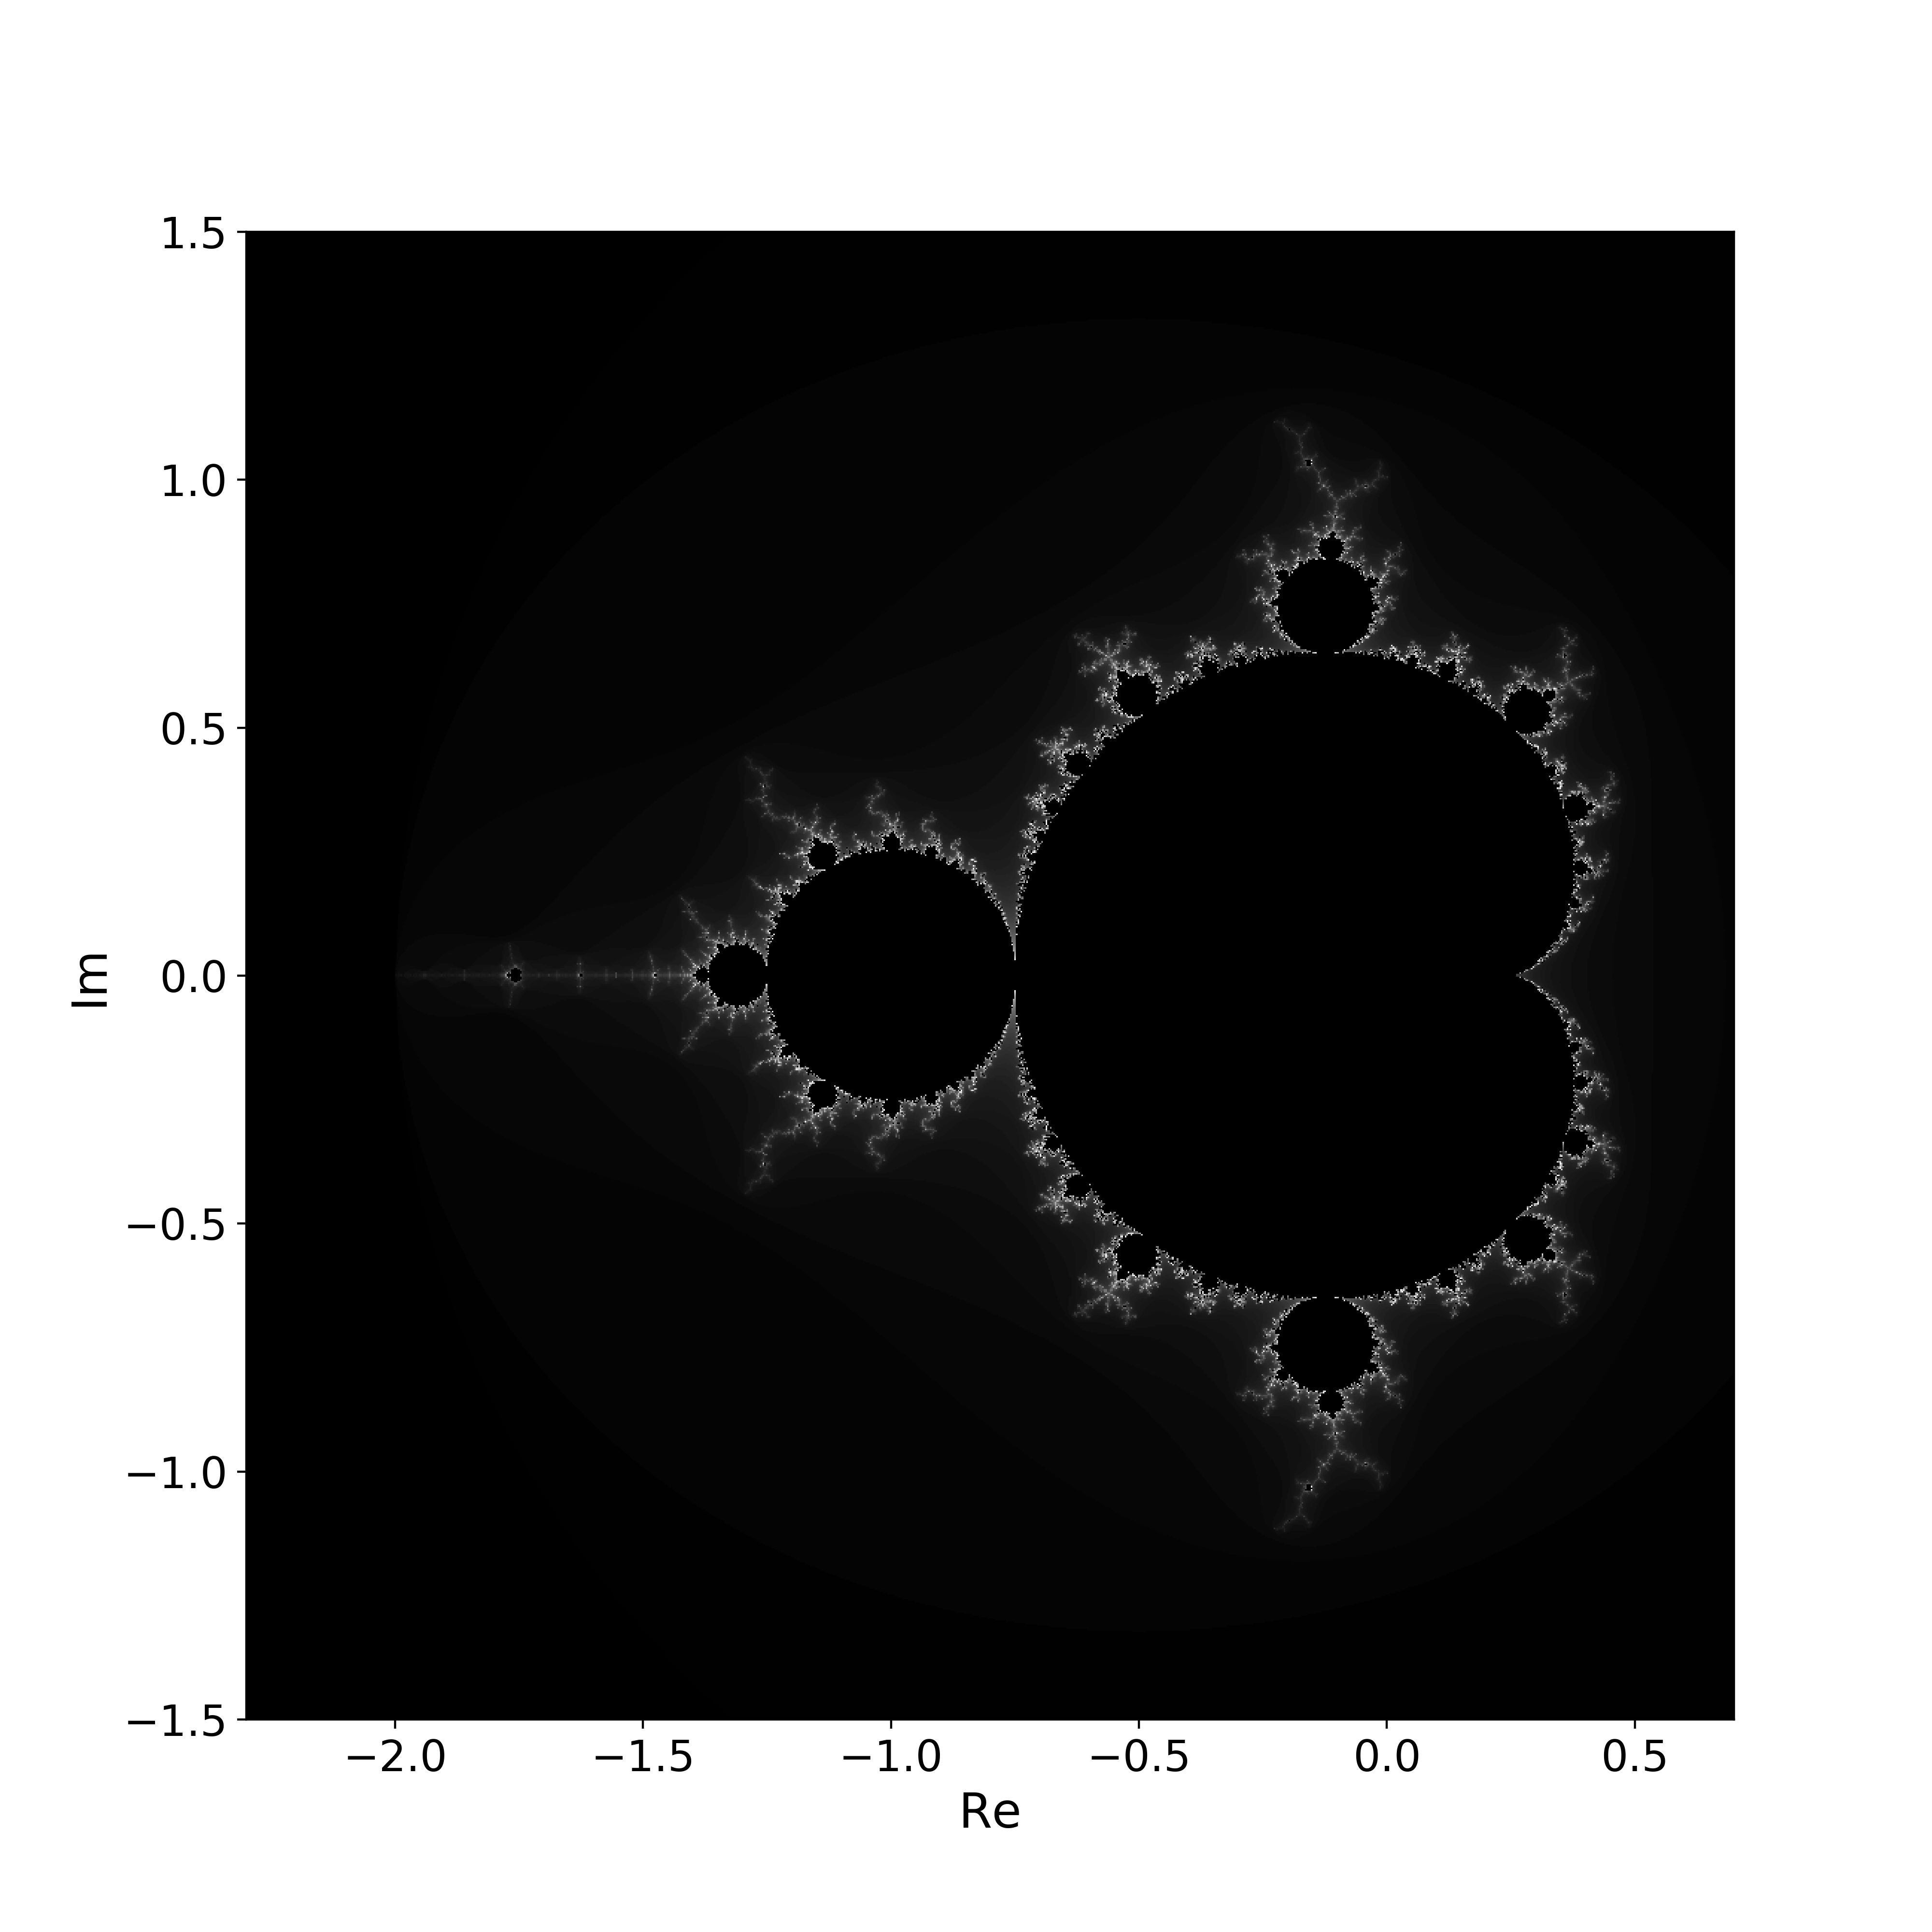
\includegraphics[width=\linewidth]{IMG/ColourGistGray.png}
  \caption{{\code{Gist\_Gray}} colour map.}
\end{subfigure}
\begin{subfigure}{.45\textwidth}
  \centering
  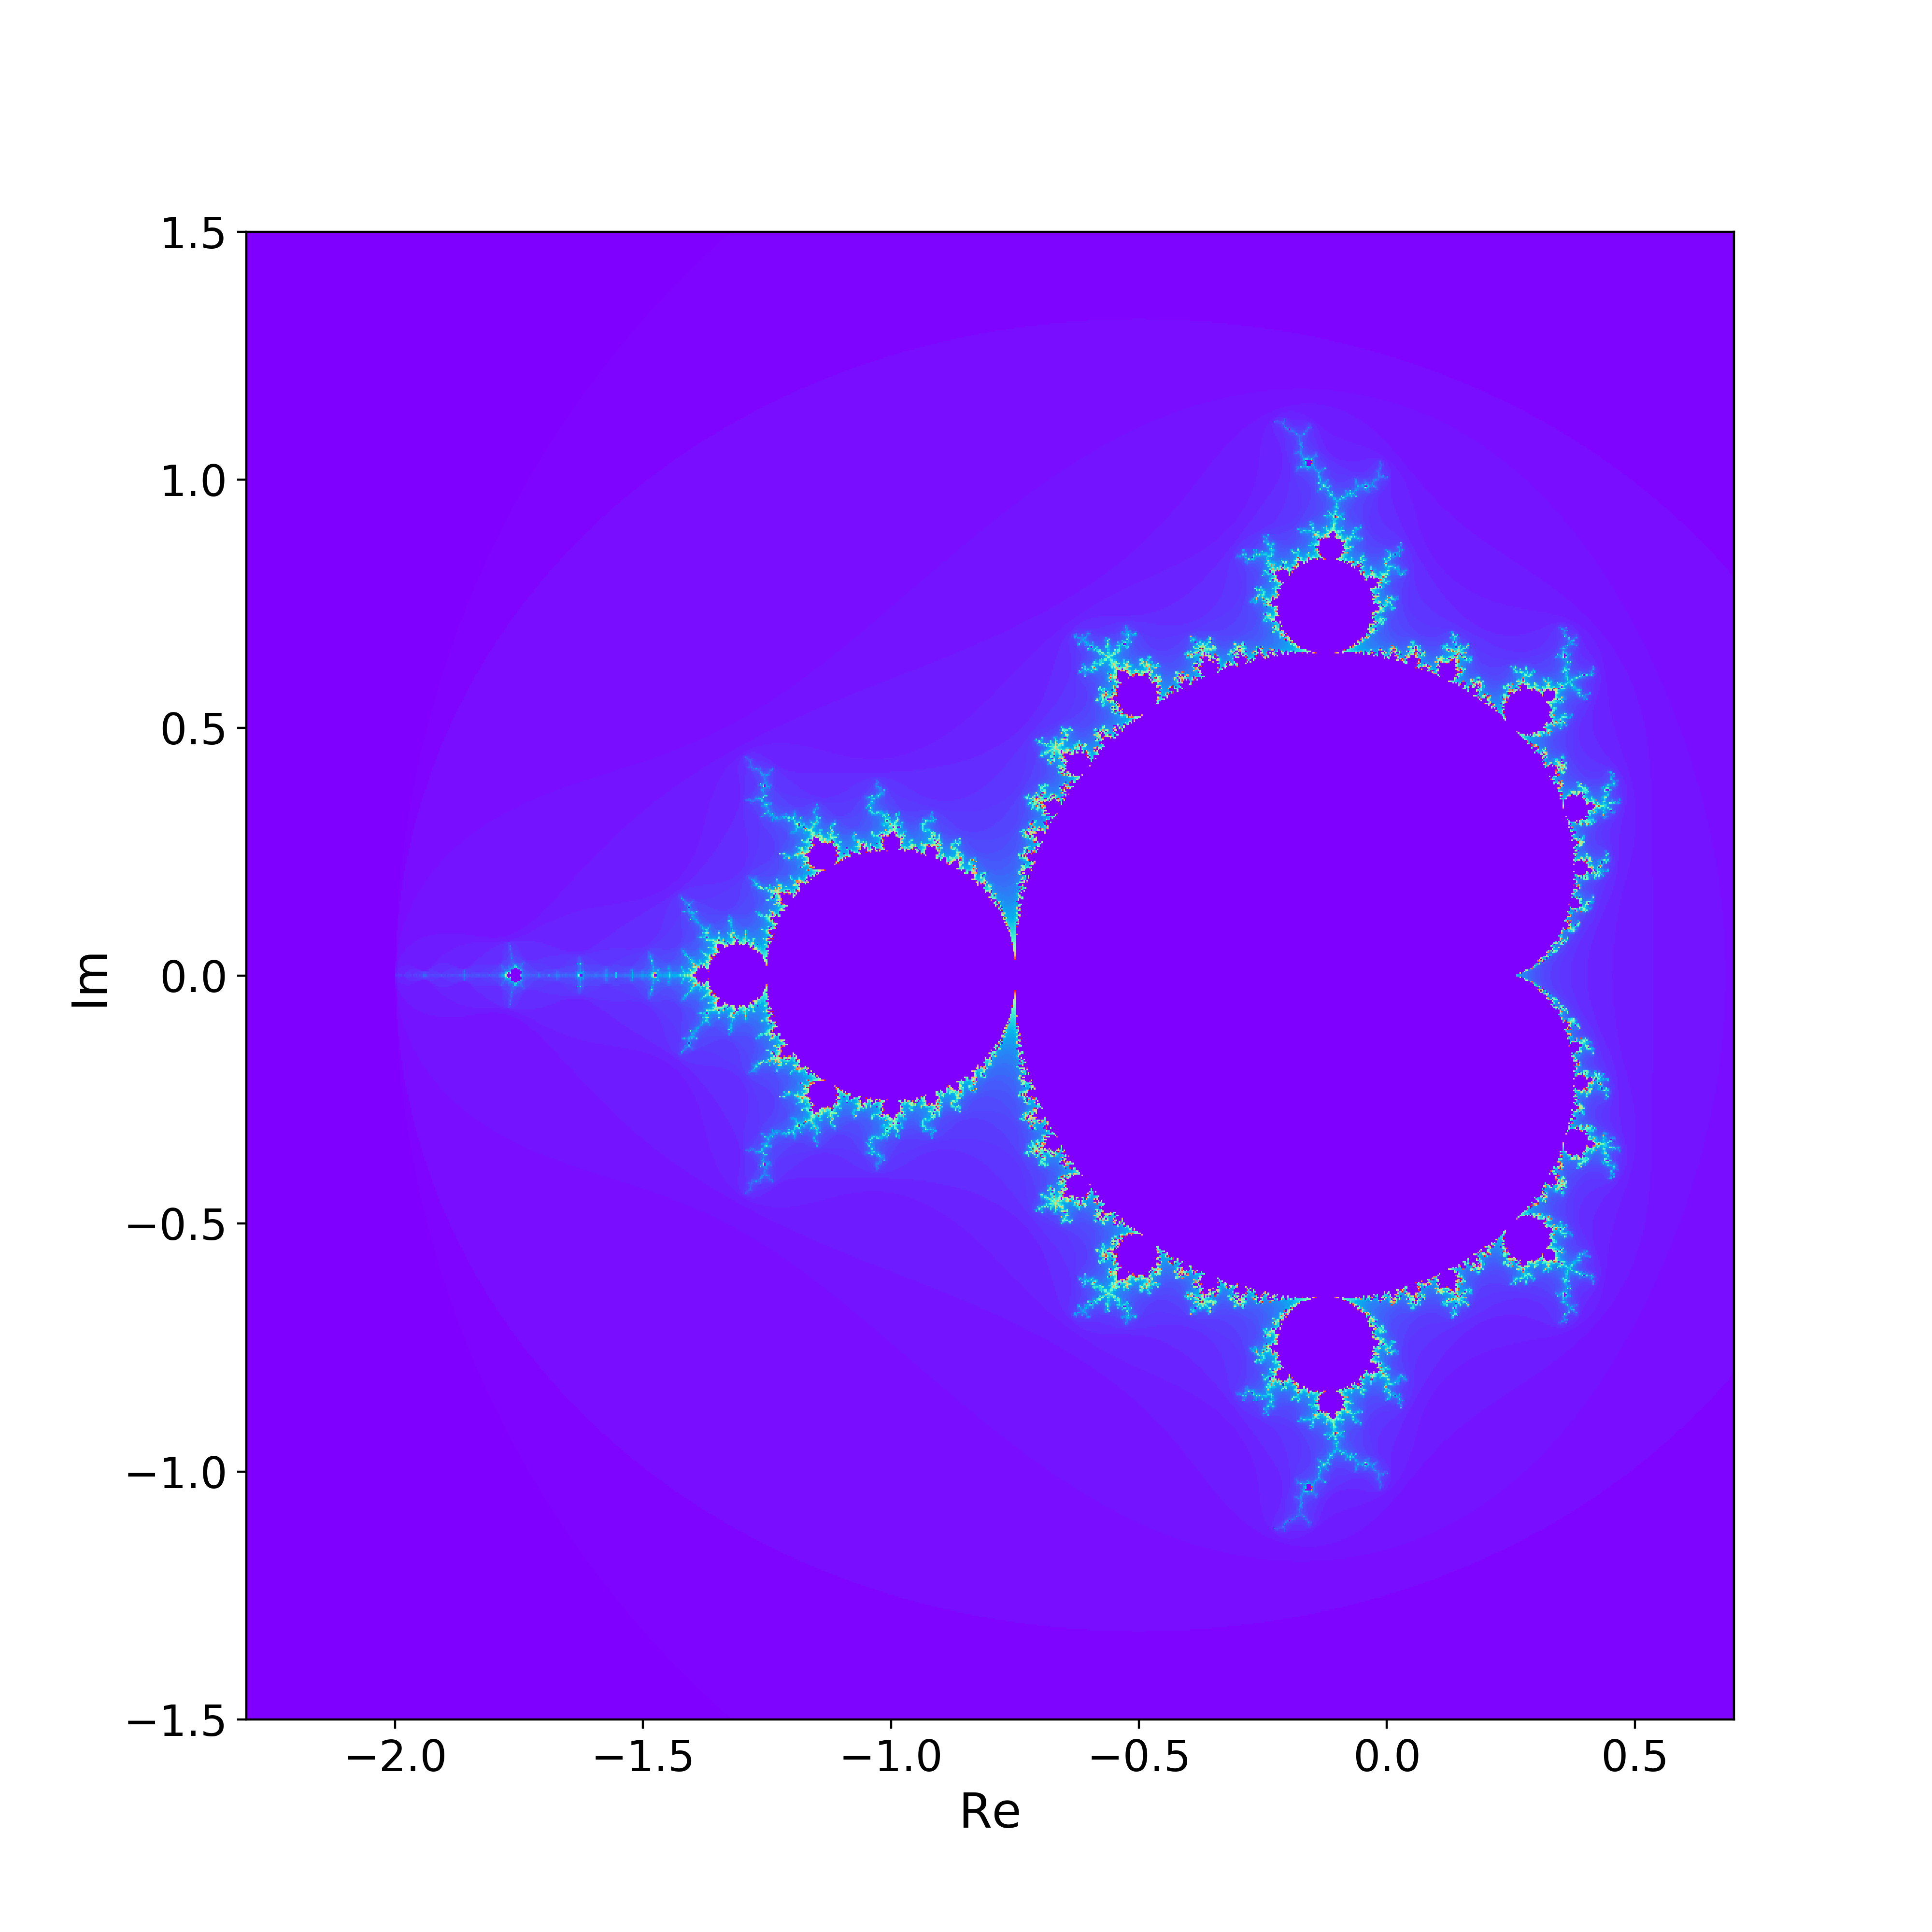
\includegraphics[width=\linewidth]{IMG/ColourInRainbow.png}
  \caption{{\code{Rainbow}} colour map.}
\end{subfigure}
\begin{subfigure}{.45\textwidth}
  \centering
  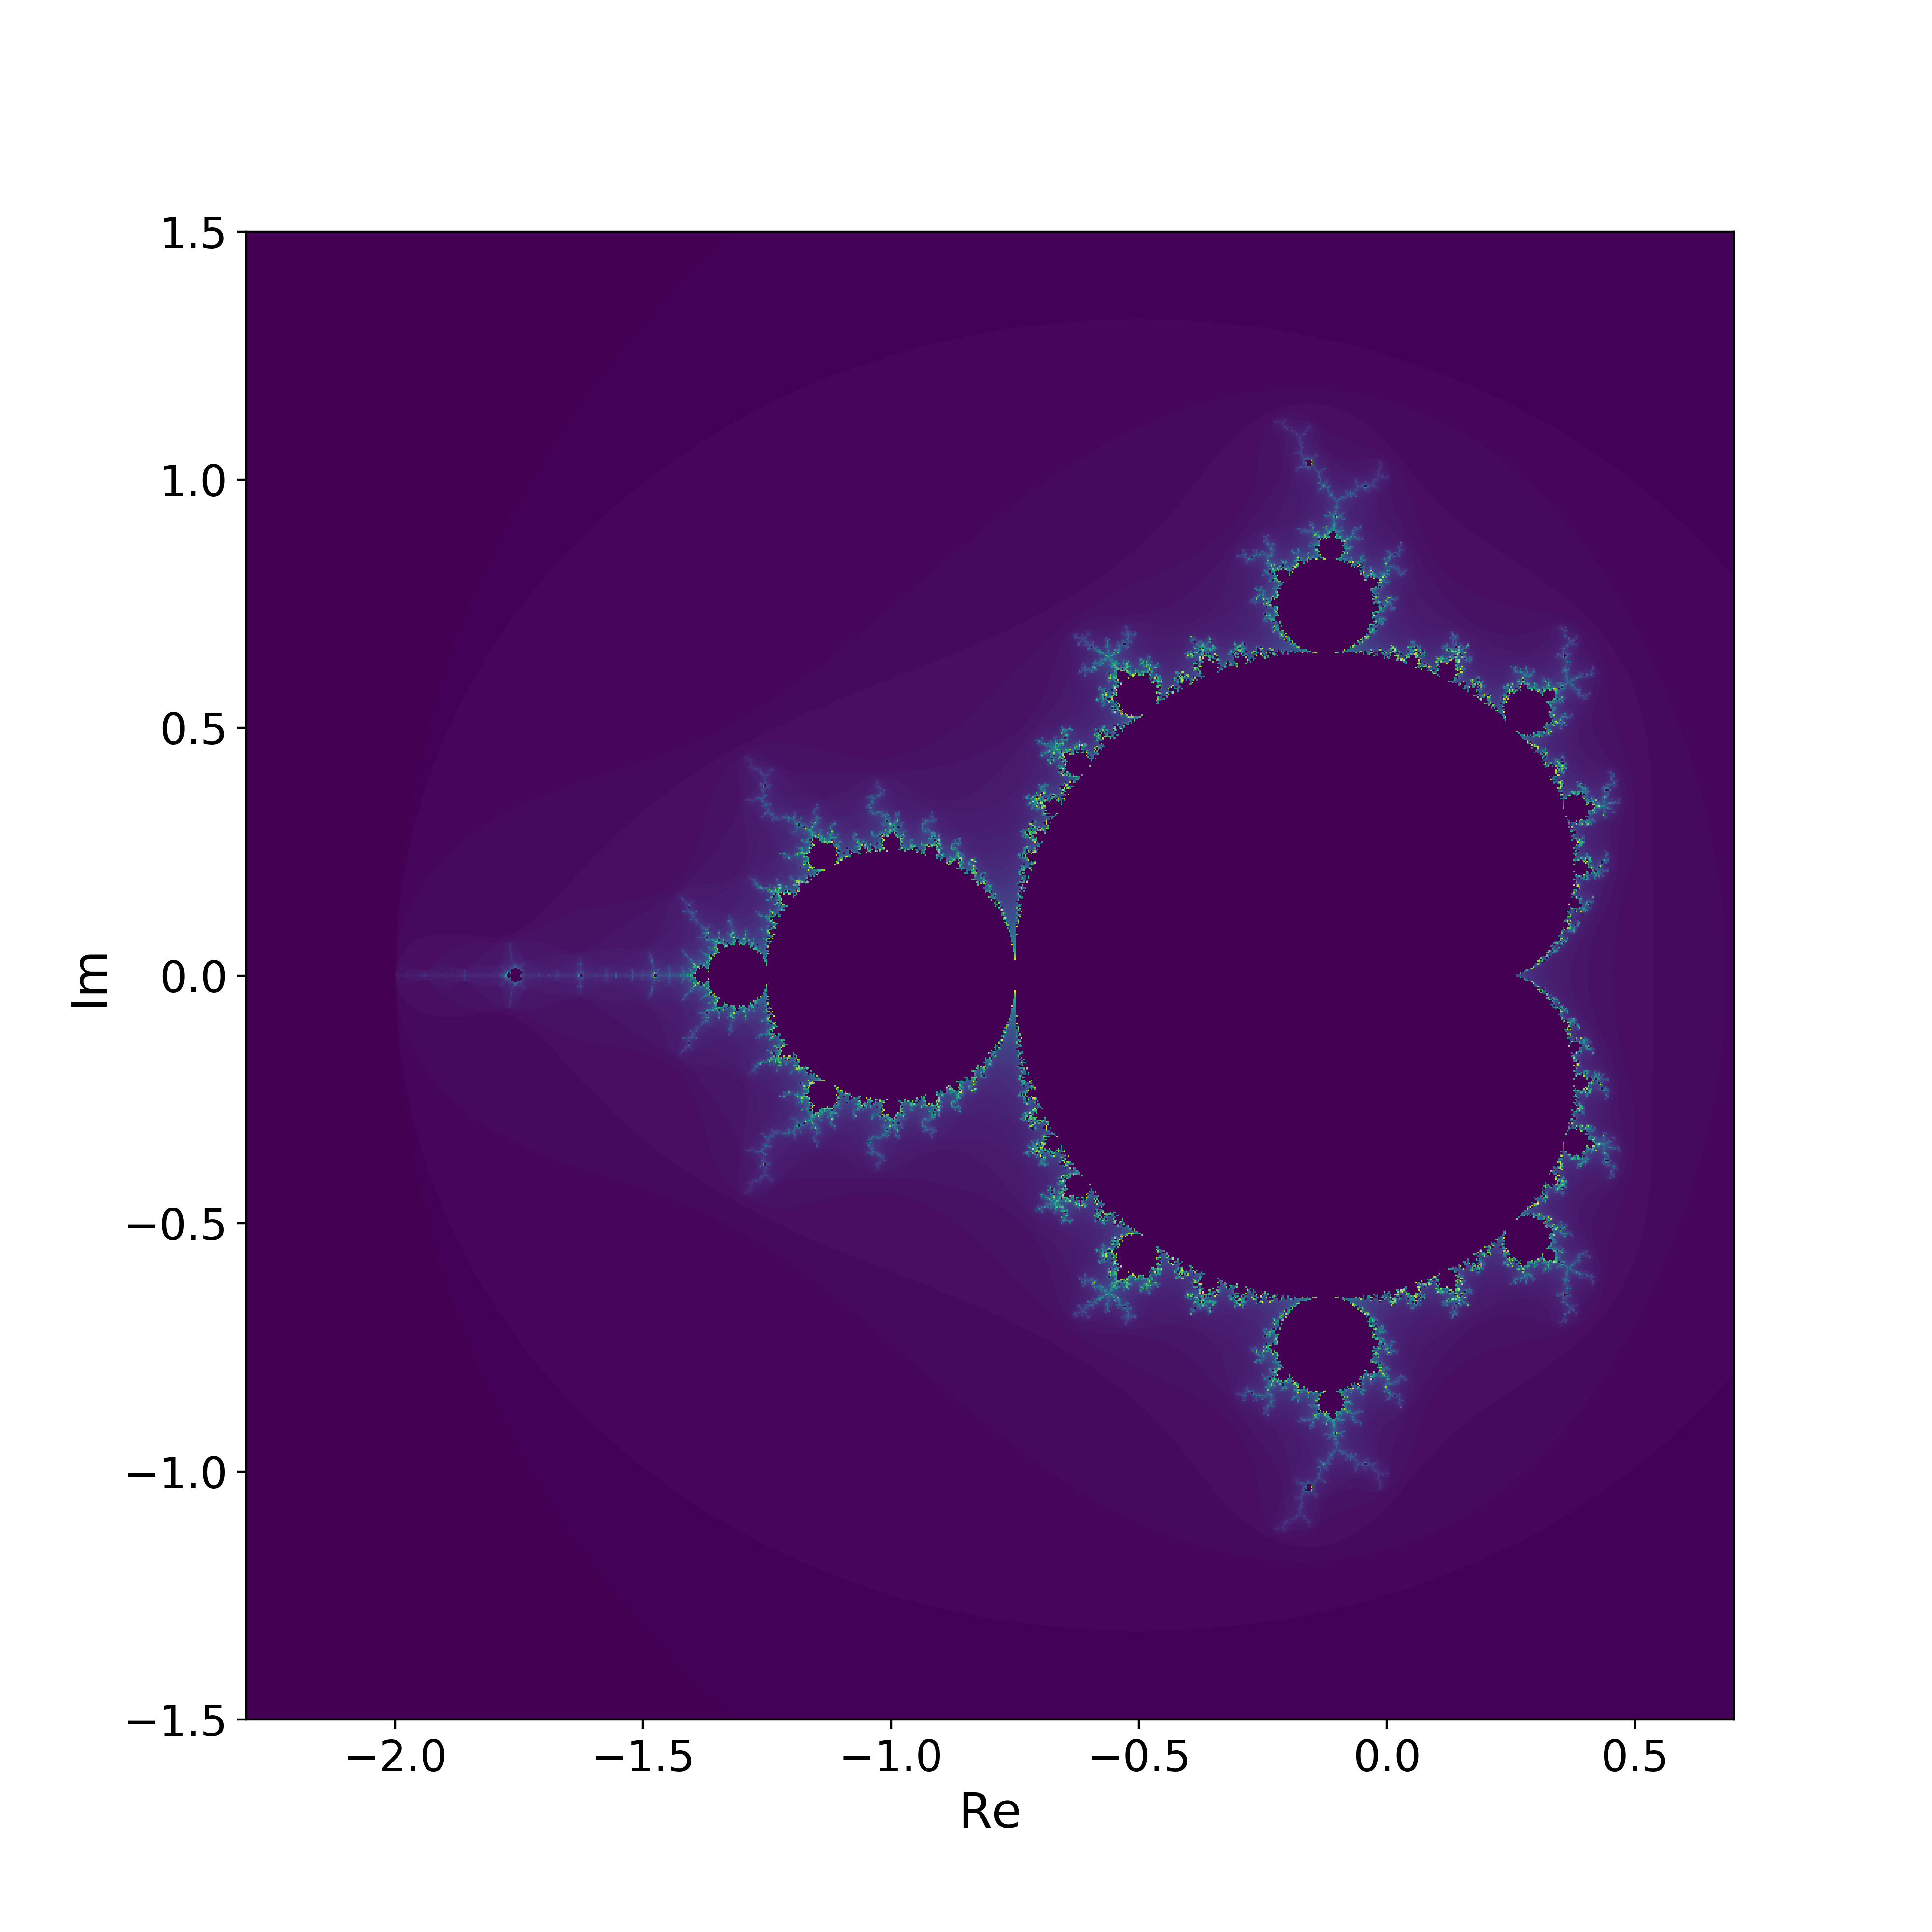
\includegraphics[width=\linewidth]{IMG/ColourViridis.png}
  \caption{{\code{Viridis}} colour map.}
\end{subfigure}
\caption{Variation of the colourmap.}
\label{FIG_Colourmap}
\end{figure}



% ------------------------------------------------------------------------------



% Special pages ----------------------------------------------------------------
\thispagestyle{plain}



% Index
\printindex
% ------------------------------------------------------------------------------


\end{document}